\documentclass{article}

\usepackage{natbib}
\usepackage{fullpage}

%\usepackage[nonatbib]{neurips_2020}

\usepackage[T1]{fontenc}    % use 8-bit T1 fonts
\usepackage{nicefrac}       % compact symbols for 1/2, etc.
\usepackage{microtype}      % microtypography
\usepackage{graphicx}

\usepackage{macro_math}
\usepackage{macro_fan}
\usepackage{stmaryrd}
\usepackage[us,12hr]{datetime}
\usepackage[utf8]{inputenc} % allow utf-8 input


\begin{document}

\title{Learning Multiple High-Dimensional Regression Tasks with Insights on Information Transfer}
\date{}
\maketitle
\date{{\ddmmyyyydate\today} at \currenttime}

% The idea is to use a shared feature space for all tasks, while each task also has a separate layer for making the prediction.
\begin{abstract}
	Hard parameter sharing for multi-task learning is widely used in empirical research despite the fact that their generalization properties have not been established in many cases. This paper studies a fundamental question to better understand this approach: How does hard parameter sharing work given multiple linear regression tasks? We develop new techniques and establish a number of new results in the high-dimensional setting, where the sample size and feature dimension become increasingly large in a fixed ratio. First, we show a sharp bias-variance decomposition of hard parameter sharing, given multiple tasks with the same features. Second, we characterize the asymptotic bias-variance limit for two tasks, even when they have arbitrarily different sample size ratios and covariate shifts. We also demonstrate that these limiting estimates for the empirical loss are incredibly accurate in moderate dimensions. Finally, we explain an intriguing phenomenon where increasing one task's sample size helps another task initially by reducing variance but hurts eventually due to increasing bias. This suggests progressively adding data for optimizing hard parameter sharing, and we validate its efficiency in text classification tasks.
\end{abstract}

\section{Introduction}\label{sec introduction}

\iffalse
%Multi-task learning is an inductive learning mechanism to improve generalization performance using related task data.
%Many state-of-the-art results in computer vision and natural language processing are obtained using multi-task learning.
Multi-task learning is a powerful approach to improve performance for many tasks in computer vision, natural language processing, and other areas \cite{C97,ZY17,R17}.
%In multi-task learning, having related task data is fundamental to its performance.
%Multi-task learning is particularly powerful when there is limited labeled data for a task to be solved, meanwhile more labeled data from different but related tasks is available.
%By combining multiple information sources, it is possible to share all the information in the same model.
In many settings, multiple source tasks are available to help with predicting a particular target task.
\todo{clarify setting is different from traditional MTL}
%For example, many applications in , and many other areas have been achieved by learning from multiple tasks together.
The performance of multi-task learning depends on the relationship between the source and target tasks \cite{C97}.
%	We define that multi-task learning provides \textit{positive transfer} if it outperforms single-task learning, or \textit{negative transfer} otherwise.
When the sources are relatively different from the target, multi-task learning (MTL) has often been observed to perform worse than single-task learning (STL) \cite{AP16,BS17}, which is referred to as \textit{negative transfer} \cite{PY09}.
While many empirical approaches have been proposed to mitigate negative transfer \cite{ZY17}, a precise understanding of when negative transfer occurs remains elusive in the literature \cite{R17}.
%This phenomenon, known as \textit{negative transfer}, is fundamental to the understanding of multi-task learning.

%Inspired by the theory, we propose an incremental training schedule to improve multi-task training.
%We consider a setting where the target task has limited labeled data and show
%On the other hand, unless the structures across task data are well-understood, applying multi-task learning on several different datasets often result in suboptimal models (or negative transfer in more technical terms).

Understanding negative transfer requires developing generalization bounds that scale tightly with properties of each task data, such as its sample size.
This presents a technical challenge in the multi-task setting because of the difference among task features, even for two tasks.
ithout a tight lower bound for multi-task learning, comparing its performance to single-task learning results in vacuous bounds.
\todo{add more technical motivation (or maybe later)}
From a practical standpoint, developing a better understanding of multi-task learning in terms of properties of task data can provide guidance for downstream applications \cite{RH19}.
%For example,
%On the other hand, uneven sample sizes (or dominating tasks) have been empirically observed to cause negative transfer \cite{YKGLHF20}.
%The benefit of learning multi-task representations has also been studied for certain half-spaces \cite{} and sparse regression \cite{}.
%When all tasks are sufficiently similar, adding more labeled data improves the generalization performance for predicting a particular task \cite{WZR20}.

%\textbf{Setup and Main Results.}
In this work, we study the bias and variance of multi-task learning in the high-dimensional linear regression setting \cite{HMRT19,BLLT20}.
Our key observation is that three properties of task data, including \textit{task similarity}, \textit{sample ratio}, and \textit{covariate shift}, can affect whether multi-task learning outperforms single-task learning (which we refer to as \textit{positive transfer}).
As an example, we vary each property in Figure \ref{fig_model_shift_phasetrans} for two linear regression tasks and measure the improvement of multi-task learning over single-task learning for a particular task.
We observe that the effect of transfer can be either positive or negative as we vary each property.
These phenomena cannot be explained using previous techniques \cite{WZR20}.
The high-dimensional linear regression setting allows us to measure the three properties precisely.
Here we define each property for the case of two tasks, while our definition applies to general settings.
We refer to the first task as the source task and the second as the target task.
\squishlist
	\item \textbf{Task similarity:} Assume that both tasks follow a linear model with parameters $\beta_1, \beta_2\in\real^p$, respectively.
	We measure the distance between them by $\norm{\beta_1 - \beta_2}$.
	\item \textbf{Sample ratio:} Let $n_1 = \rho_1 \cdot p, n_2 = \rho_2 \cdot p$ be the sample size of each task, where $\rho_1, \rho_2>1$ are both fixed values that do not grow with $p$.
	We measure the source/target sample ratio by $\rho_1 / \rho_2$.
%	Importantly, $\rho_2$ can be a small constant (say $2$) to capture the need for more labeled data.
	\item \textbf{Covariate shift:} Assume that the task features are random vectors with positive semidefinite covariance matrices $\Sigma_1\in\real^{p\times p}$ and $\Sigma_2\in\real^{p\times p}$, respectively.
	%$x = \Sigma_i^{1/2}z$, where $z\in\real^p$ consists of i.i.d. entries with mean zero and unit variance, and is a positive semidefinite matrix.
	We measure covariate shift with matrix $\Sigma_1^{1/2}\Sigma_2^{-1/2}$.
\squishend
\fi


Hard parameter sharing (HPS) for multi-task learning is widely used in empirical research and goes back to the seminal work of \citet{C97}.
Recent work has revived interest in this approach because it improves performance and reduces the cost of collecting labeled data \cite{MTDNN19,ZSSGM18}.
It is generally applied by sharing the feature layers between all tasks while keeping an output layer for every task.
Often, hard parameter sharing offers two critical advantages if successfully applied.
(i) It reduces model parameters since all tasks use the same feature space.
(ii) It reduces the amount of labeled data needed from each task by augmenting the entire training dataset.

Hard parameter sharing offers great intuitive appeal as an inductive transfer mechanism.
It reduces overfitting by acting as a regularizer \cite{R17}.
For example, by restricting the shared space's size, HPS encourages information sharing among multiple tasks \cite{KD12}.
Another source of inductive bias comes from the tasks and depends on datasets' properties such as sample sizes and task covariances \cite{WZR20}.
However, how these dataset properties impacts HPS has not been established.
%It becomes increasingly important to understand HPS' formal generalization properties.
Part of the challenge may be that HPS' generalization performance depends intricately on the sample size ratios and covariate shifts between tasks, not amenable to standard concentration results.
Previous results based on Rademacher complexity or VC dimensions have considered when all tasks' sample sizes are equal to logarithm factors of feature dimension \cite{B00,MPR16}, and when all tasks' sample sizes increase simultaneously \cite{AZ05,M06}.
%For, the generalization error scales down as the sample sizes of all tasks increase, when applied to the multi-task setting \cite{B00,AZ05,M06,MPR16,WZR20}.

This paper presents new techniques to study hard parameter sharing and establish a number of new results.
We consider regression analysis, which is arguably one of the most fundamental problems in statistics and machine learning.
We are interested in the \textit{high-dimensional} setting, where each dataset's sample size and feature dimension grow linearly at a fixed ratio.
This is motivated by many multi-task learning applications, where the amount of labeled data from each dataset is usually insufficient for learning a single task.
For example, this is the case if a dataset's sample size is only a small constant factor of the feature dimension.
The high-dimensional setting is challenging but is crucial for understanding how datasets' sample sizes impact generalization performance.

\subsection{Problem Formulation and Main Results}

%Suppose we have $t$ labeled regression tasks. %where $t$ is a fixed value that does not grow with the feature dimension $p$.
%For each task $k$ from $1$ to $t$, we have $n_k$ samples $x_1, x_2, \dots, x_{n_k}$ that are all $p$-dimensional feature vectors with real-valued labels $y_1, y_2, \dots, y_{n_k}$.
%Without loss of generality, we focus on predicting the $t$-th task and refer the $t$-th task as the target.
%We refer to task $1$ to task $t-1$ as source tasks.
%We assume that the labels of each task $k$ satisfy the linear model with unknown parameters $\beta_k\in\real^p$, that is,
%	\[ y_i = x_i^{\top}\beta_k + e_i, \text{ for all } 1 \le i \le n_k, \]
%where $e_i$ denotes random noise with mean zero and variance $\sigma^2$.
%To write the above notations more succiently, let $X_k \in \real^{n_k \times p}$ denote the covariates that consists of a feature vector in every row.
%Let
%	\be\label{model_YvsX} Y^{(k)} = X^{(k)} \beta_k + \varepsilon_k, \text{ for all } 1\le k \le t \ee denote the label vector of task $k$ and $\varepsilon_k$ denote an i.i.d. random vector with mean zero and variance $\sigma^2$.
%Following \citet{HMRT19} and \citet{BLLT20},
%In the high-dimensional linear regression setting (e.g. ), the features of the $k$-th task, denoted by $X_k\in\real^{n_i\times p}$, consist of $n_k$ feature vectors given by $x_1, x_2, \dots, x_{n_k}$.
%we assume that for each task $k$ from $1$ to $t$, each feature vector $x_i = \Sigma^{1/2}_k z_i$ for $i = 1, \dots, n_k$, where $z_i\in\real^p$ is an i.i.d. random vector with  mean zero and unit variance.
%Recall that $\Sigma_k$ is the population covariance matrix task $k$'s feature vectors.
%Let $\Sigma_k = U_k D_k U_k^{\top}$ denote the singular value decomposition of $\Sigma_k$.
%We denote $\Sigma_k = U_k D_k^{1/2}$ as the square root of $\Sigma_k$.
%The sample size of task $k$, given by $n_k$, is equal to $\rho_k\cdot p$ for a fixed value $\rho_k$ that does not grow with feature dimension $p$.
%This setting is also known as the high-dimensional linear regression setting in the literature.
%There are two motivations for studying the high-dimensional linear regression setting for multi-task learning.
%First, this setting captures salient properties of modern large-scale datasets, where the sample sizes are usually on the order of tens to hundreds of the number of features \cite{sur2019modern}.
%Second, as we will see soon in Section \ref{sec_general}, we can derive precise asymptotics of the generalization error that scale with properties of the task data such as sample sizes.
%The labels $Y_k = X_k \beta_k + \varepsilon_k$, where $\beta_k$ denotes the linear model parameters and $\varepsilon_k$ denotes i.i.d. noise with mean zero and variance $\sigma^2$.
%Recall that we have $t$ labeled training datasets, denoted by $(X_1, Y_1), (X_2, Y_2), \dots, (X_t, Y_t)$, where $X_i\in\real^{n_i\times p}$ and $Y_i\in\real^{n_i}$ for $1\le i\le t$.
%Following \cite{HMRT19,BLLT20}, we assume that for each task $i = 1,2,\dots,t$,  every feature vector is generated as $x = \Sigma_i^{1/2} z$, where $z\in\real^p$ is a random vector with i.i.d. entries of mean zero and unit variance and $\Sigma_i\in\real^{p\times p}$ is a positive semidefinite matrix.
%Without loss of generality, let the $t$-th task be the target task.

Regression analysis is arguably one of the most fundamental methods in statistics and machine learning.
In many multi-task learning applications, the amount of labeled data from each dataset is usually insufficient for learning a single task.
For example, this is the case if a dataset's sample size is only a small constant factor of the feature dimension \cite{GLUE}.
In this paper, we consider multi-task learning in a \textit{high-dimensional} linear regression setting, where each dataset's sample size and the feature dimension grow linearly at a fixed ratio.
The high-dimensional setting is challenging but is crucial for understanding how datasets' sample sizes impact generalization performance.
We assume that there are multiple datasets that all follow a (potentially different) linear model.
In each dataset, suppose the feature vector $x = {\Sigma}^{1/2} z$, where $z \in \real^p$ has i.i.d entries with mean zero, unit variance, and covariance $\Sigma \in\real^{p \times p}$ that is deterministic and positive semidefinite.

We study a hard parameter sharing architecture to learn jointly from multiple datasets.
In this architecture, there is a shared feature representation layer $B\in\real^{p\times r}$ for all tasks and a separate output layer $A_i \in \real^r$ for every task $i$.
Suppose we have $t$ datasets.
For each dataset $i$ from $1$ to $t$, let $n_i$ denote its sample size, $X^{(i)} \in \real^{n_i \times p}$ denote its feature covariates, and $Y^{(i)} \in \real^{n_i}$ denote all the labels.
%The width of $B$, denoted by $r$, plays an important role in regularization.
%As observed in Proposition 1 of \citet{WZR20}, if $r \ge t$, there is no regularization effect.
%Hence, we assume that $r < t$ in our study.
%For example, when there are only two tasks, $r = 1$ and $B$ reduces to a vector whereas $W_1, W_2$ become scalars.
Let $A = [A_1, A_2, \dots, A_t] \in \real^{r \times t}$.
We study the following optimization objective.
%	\item Separate each dataset $(X_i, Y_i)$ randomly into a training set $(X_i^{tr}, Y_i^{tr})$ and a validation set $(X_i^{val}, Y_i^{val})$.
%	The size of each set is described below.
%	\item Learn the shared layer $B$: minimize the training loss over $B$ and $W_1, \dots, W_t$, leading to a local minimum of $B$ that depends on $W_1, \dots, W_t$, denoted by $\hat{B} = \hat{B}(W_1, \dots, W_t)$.
\begin{align}\label{eq_mtl}
			f(A, B) = \sum_{i=1}^t \norm{X^{(i)} B A_i - Y^{(i)}}^2.
\end{align}
Given a solution $\hat{A}, \hat{B}$ from the above optimization, let $\hat{\beta}_i^{\MTL} = \hat{B} \hat{A}_i$ denote the hard parameter sharing (HPS) estimator for task $i$.
The critical questions here are:
(i) how well does the estimator work? In particular, how does the performance of the estimator scale with sample size?
(ii) for datasets with different sample sizes and covariate shifts, how do they impact the estimator?


%	\item Learn the output layers $W_1, W_2, \dots, W_t$: set $B = \hat{B}$ and minimize the training loss over $W_1, W_2, \dots, W_t$.
%		{\begin{align}\label{eq_mtl_eval}
%			g(W_1, \dots, W_t) = \sum_{k=1}^t \norm{X_k \hat{B} W_k - Y_k}^2.
%		\end{align}}
%\end{enumerate}
%Let $\hat{\beta}_t^{\MTL}$ denote the multi-task learning estimator obtained from the procedure above.
%By contrast, let $\hat{\beta}_t^{\STL} = (X_t^{\top}X_t)^{-1}X_t^{\top}{Y_t}$ denote the single-task learning estimator. % denoted by $L(\hat{\beta}_t^{\STL})$.
%where $B\in\real^{p\times r}$ and $W_k\in\real^r$ for every $1\le k\le t$.
%Following , we assume that $r < t$, because otherwise minimizing $f(\cdot)$ could result in $BW_i$ being the single-task optimum.
%\smallskip
%\noindent\textit{Remark.}
%In general, the multi-task learning objective $f(\cdot)$ is non-convex with respect to $B$ and $W_1, \dots, W_t$.
%Therefore, we first minimize $B$ in equation \eqref{eq_mtl} and then minimize $W_k$ given $B$ in equation \eqref{eq_mtl_eval}.
%For our results later in Section \ref{sec_general} and \ref{sec_special}, we will identify tractable cases and provide guarantees to the above procedure.
%\paragraph{Problem statement.}
%We focus on predicting a particular task, say the $t$-th task, without loss of generality.
%For an estimator $\hat{\beta}$ of the target task model $\beta_t$, we define the prediction loss of the estimator $\hat{\beta}$ as
%	{\begin{align}\label{eq1_prediction_loss}
%		\te(\hat{\beta}) = \exarg{x = \Sigma_t^{1/2} z}{({x}^{\top}\hat{\beta} - {x}^{\top}\beta_t)^2}
%		= \bignorm{\Sigma_t^{1/2} (\hat{\beta} - \beta_t)}^2,
%	\end{align}}%
%where $x = \Sigma_t^{1/2} z$ denotes a random feature vector with covariance $\Sigma_t$.
%In the above equation, $x^{\top}\beta_t$ is the true label of $x$.
%= (\hat{\beta} - \beta_t)^{\top}\Sigma_t(\hat{\beta} - \beta_t)
%We say that the source tasks provide a \textit{positive transfer} to the target task if the prediction loss of the MTL estimator is lower than that of the STL estimator, that is, if
%	\[ L(\hat{\beta}_t^{\MTL}) > L(\hat{\beta}_t^{\STL}). \]
%On the other hand, we say that the source tasks provide a \textit{negative transfer} to the target task if $L(\hat{\beta}_t^{\MTL}) < L(\hat{\beta}_t^{\STL})$.
%Our goal is to study when the source tasks provide a positive transfer to the target task.
%More specifically, we study how varying properties of task data including task similarity, sample ratio, and covariate shift affects information transfer in multi-task learning.

%We begin by defining our problem setup including the multi-task estimator we study.
%Then, we describe the bias-variance tradeoff of the multi-task estimator and connect the bias and variance of the estimator to \textit{task similarity}, \textit{sample size}, and \textit{covariate shift}.
%Finally, we show a tight concentration bound for the bias and variance quantities using random matrix theory.

%\subsection{Problem Formulation}

%In the worst case, the optimization objective \eqref{eq_mtl} is non-convex in $A$ and $B$ (e.g. matrix completion is a special case for suitably designed $X^{(i)}, Y^{(i)}$).
%Therefore, we work in cases where a global and/or local minimum characterization is possible

\paragraph{Main results.}
Our first result (Theorem \ref{thm_many_tasks}) applies to the multi-label prediction setting where all datasets have the same features, and we want to make multiple predictions (e.g. \cite{hsu2009multi}).
We analyze the global minimum of $f(A, B)$, and provide a sharp generalization bound for its (out-of-sample) prediction loss for any task.
This case is tractable even though in general, $f(A, B)$ is non-convex in $A$ and $B$ (e.g. matrix completion is a special case for suitably designed $X^{(i)}, Y^{(i)}$).
We show that the prediction loss of hard parameter sharing admits a clean bias-variance decomposition.
Our results imply that hard parameter sharing helps by reducing variance compared to single-task learning, but hurts by increasing bias.
Our second result (Theorem \ref{thm_main_RMT}) applies to two tasks with arbitrarily different sample sizes and population covariance matrices.
We analyze the local minimum of $f(A, B)$ and provide a sharp generalization bound for both tasks' prediction loss.
Despite its simplicity, we show several rich phenomena by varying sample sizes and covariate shifts in this setting.
See Figure \ref{fig_intro_sample_size} for an illustration.

\begin{figure}[!t]
	\begin{subfigure}[t]{0.5\textwidth}
		\centering
		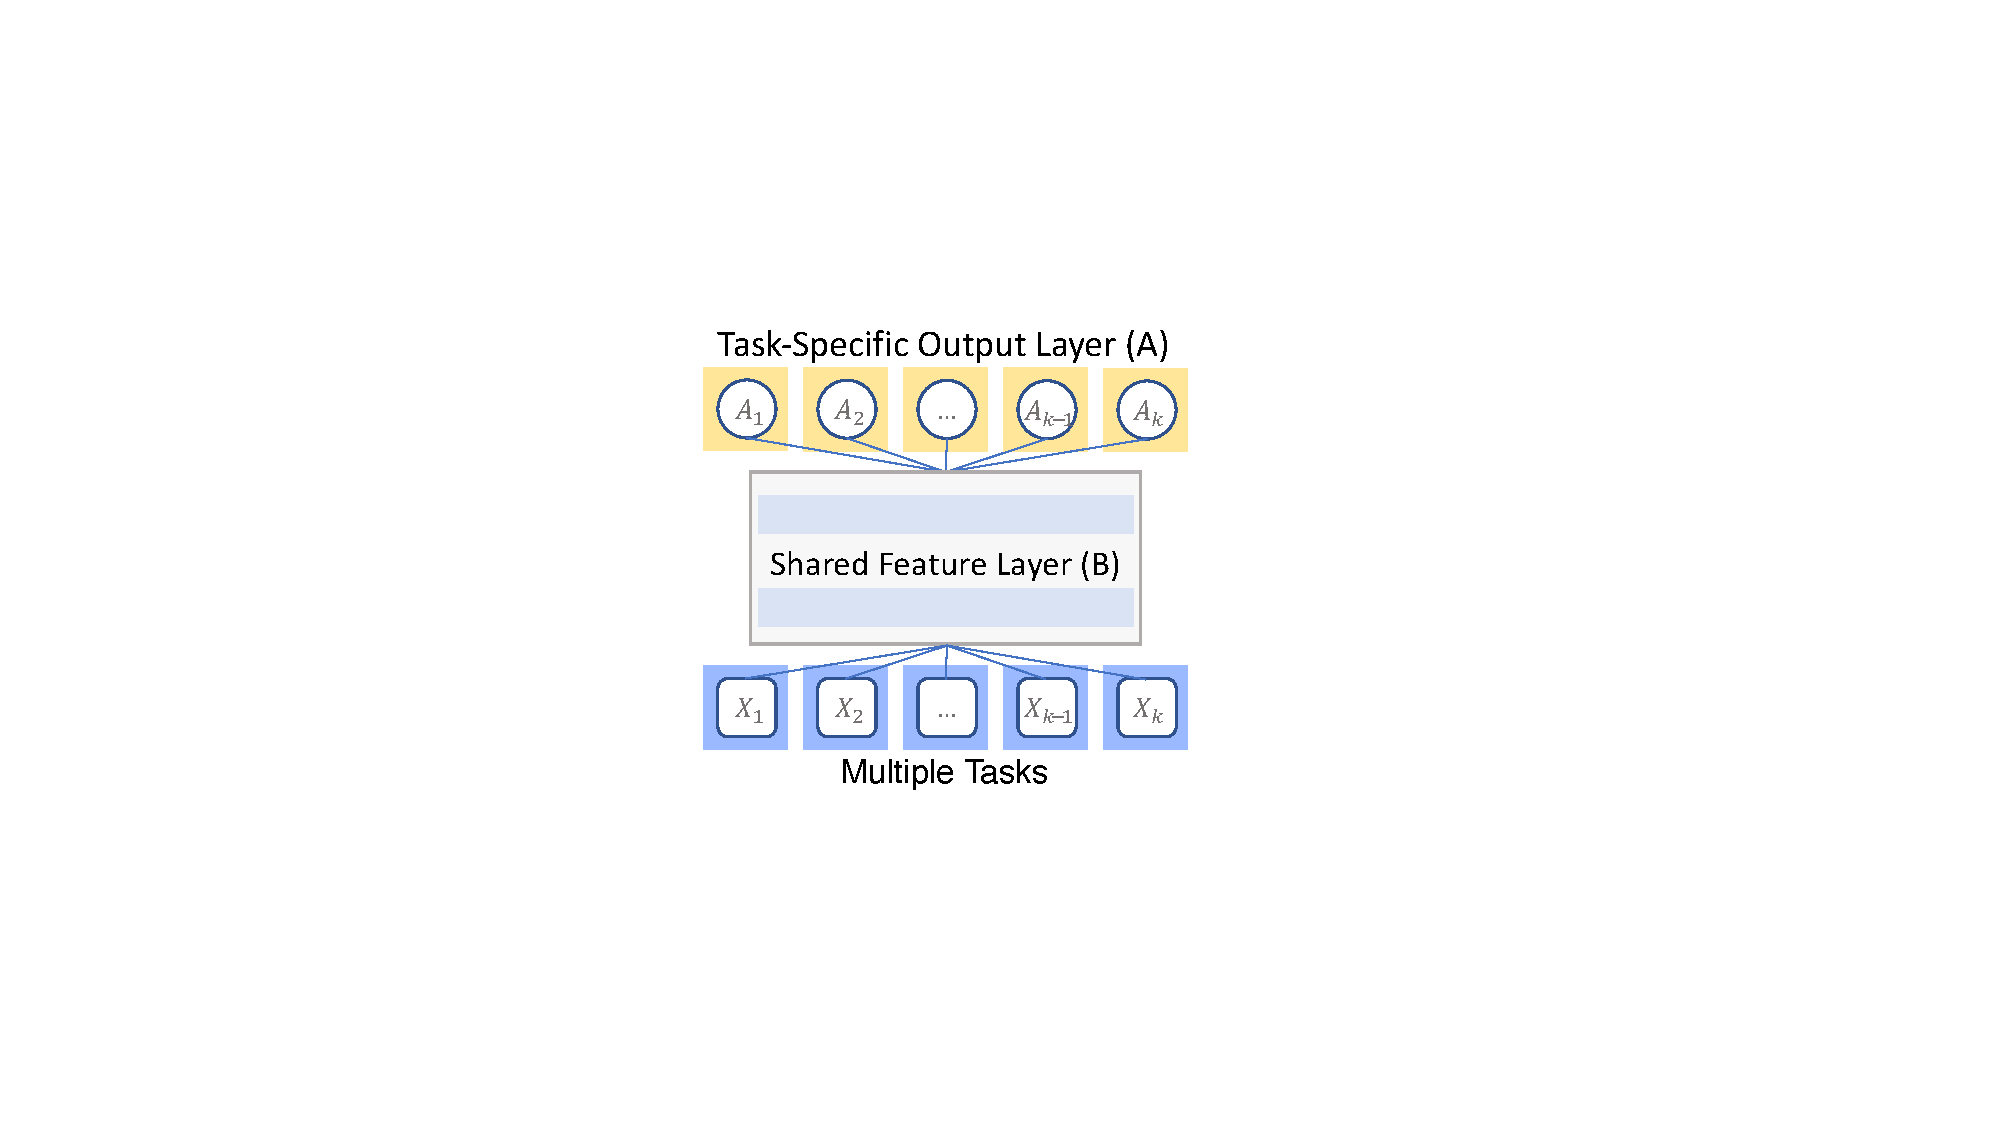
\includegraphics[width=0.5\textwidth,valign=t]{figures/mtl_model_arch.pdf}
		\caption{A hard parameter sharing architecture}
	\end{subfigure}\hfill
	\begin{subfigure}[t]{0.5\textwidth}
		\centering
		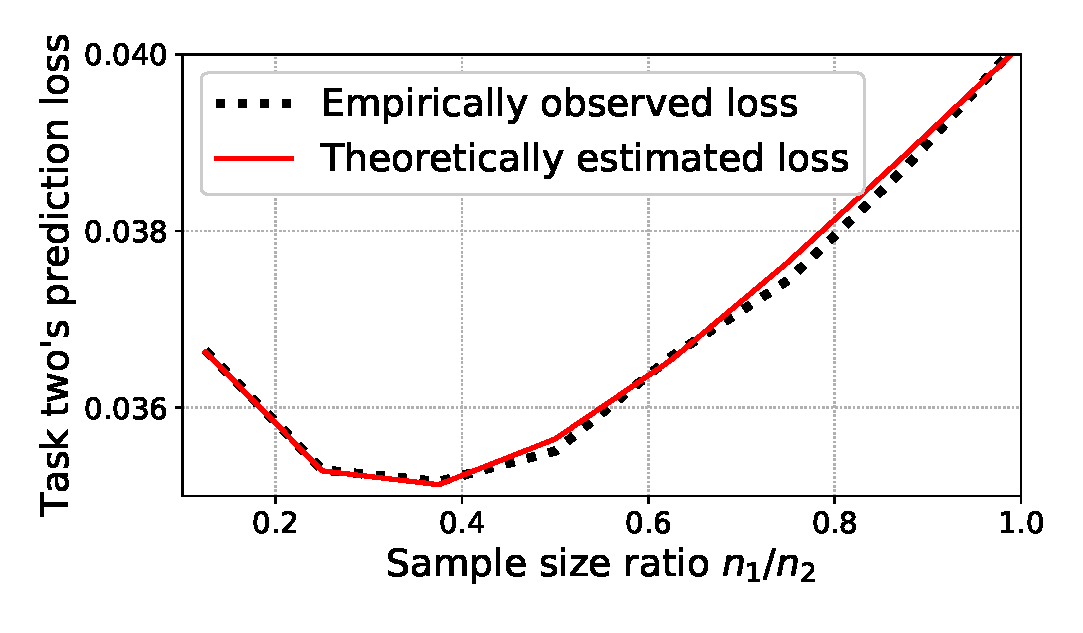
\includegraphics[width=0.713\textwidth,valign=t]{figures/sample_ratio_c2_400.eps}
		\caption{Varying sample size ratio}
		\label{fig_intro_sample_size_b}
	\end{subfigure}
	\caption{An illustrative example of our result:
	Consider the prediction loss of hard parameter sharing (left) for task two, given two linear regression tasks.
	Increasing task one's sample size decreases task two's prediction loss initially, but increases afterward. This phenomenon occurs due to different bias-variance tradeoffs as the sample size ratio increases. Our result provides an estimated loss (solid line) that accurately matches the empirical loss (dotted line).
	See Section \ref{sec_simulation} for the precise setting.}
	\label{fig_intro_sample_size}
\end{figure}

Consequently, we observe qualitative properties of hard parameter sharing for varying datasets' properties using our precise loss estimates.
\begin{enumerate}
	\item \textit{Sample efficiency (Example \ref{ex_same_cov})}:
	One advantage of combining multiple datasets is that the requirement for labeled data reduces compared to STL, a phenomenon that \citet{ZSSGM18} has observed empirically.
	Our results further imply that HPS's sample efficiency depends on model-specific variance vs. noise variance. It is generally high when the noise variance is large compared to model-specific variance across tasks.
	\item \textit{Sample size ratio (Example \ref{ex_sample_ratio})}: Increasing one task's sample size does not always help reduce another task's loss. In a simplified setting, we find that the task loss either decreases first before increasing afterward or decreases monotonically depending on how much bias increases. These two trends result from different tradeoffs between increasing bias and decreasing variance.
	\item \textit{Covariate shift (Example \ref{ex_covshift})}: In addition to sample sizes, variance also scales with the covariate shift between different datasets. For a high sample size ratio, HPS's  variance is smallest when there is no covariate shift. Counterintuitively, for a low sample size ratio, having covariate shifts reduces variance through a complementary spectrum.
\end{enumerate}

%First, we develop tight bounds for the bias and variance of the multi-task estimator for two tasks by applying recent development in random matrix theory \cite{erdos2017dynamical,isotropic,Anisotropic}.
%We observe that the variance of the multi-task estimator is \textit{always smaller} than single-task learning, because of added source task samples.
%On the other hand, the bias of the multi-task estimator is \textit{always larger} than single-task learning, because of model distances.
%Hence, the tradeoff between bias and variance determines whether the transfer is positive or negative.
%We provide a sharp analysis of the \textit{variance} that scales with sample size and covariate shift.
%We extend the analysis to the bias, which \textit{in addition} scales with {task similarity}.
%Combining both, we analyze the bias-variance tradeoff for two tasks in Theorem \ref{thm_main_informal} and extend the analysis to many tasks with the same features in Theorem \ref{thm_many_tasks}.
%For the setting of two tasks, we show how the variance of the multi-task estimator  scales with sample size and covariate shift in the following result.
%\textit{Our first contribution} is to develop a concentration bound that arises naturally from the bias-variance tradeoff of $\hat{\beta}_t^{\MTL}$ for two tasks.
%Let $\hat{\beta}_t^{\STL}$ denote the single-task estimator.
%Without loss of generality, let the $t$-th task denote the target task.
%Importantly, the target task's data size is a fixed constant times $p$ in the high-dimensional setting.
%Hence adding more labeled data can help improve its test performance.
%$B\in\real^{p\times r}$
%$\set{W_i \in \real^{r}}_{i=1}^t$

%Concretely, we show a tight bound on the trace of $(X_1^{\top}X_1 + X_2^{\top}X_2)^{-1}$, which
%Theorem \ref{lem_cov_shift_informal} allows us to analyze the bias-variance tradeoff of the multi-task estimator for two settings:
%(i) two tasks with arbitrary covariate shift; (ii) many tasks with no covariate shift.

%We shall assume that each task data follows a linear model, i.e. $y_i = X_i \beta_i + \varepsilon_i$, $1\le i\le k$.
%Here $\beta_i\in\real^p$ is the model parameter for the $i$-th task.
%Each row of $X_i\in\real^{n_i\times p}$ is assumed to be drawn i.i.d. from a fixed
%distribution with covariance matrix $\Sigma_i$.

%We extend our result to the transfer learning
%in the setting of high-dimensional linear regression.
%by pooling source task representations into the shared body of the hard parameter sharing architecture, following
%setting of Taskonomy by Zamir et al. \cite{ZSSGM18}.
%We prove that the bias of the transfer learning estimator is given by the projection of $\beta_t$ to the orthogonal subspace spanned by $\set{\beta_i}_{i=1}^{t-1}$.
%These results are described more precisely in Section \ref{sec_main}.

%Second, we explain the phenomena in Figure \ref{fig_model_shift_phasetrans} in isotropic and covariate shifted settings.
%We observe that negative transfer occurs as (a) \textit{task similarity}: tasks become more different; (b) \textit{data size}: source/target data size increases.
%\textbf{Task similarity:}
%\textbf{Data sizes:}
%\textbf{Covariate shift:}
%Furthermore, MTL performance is negatively affected when (c) \textit{covariate shift}: the covariance matrices of the two tasks become more different.
%\squishlist
%	\item We provide conditions to predict the effect of transfer as a parameter of model distance $\norm{\beta_1-\beta_2}$ (Section \ref{sec_similarity}).
%	As model distance increases, the bias becomes larger, resulting in negative transfer.
%	Our result predicts most of the empirical observations in Figure \ref{fig_model_shift} correctly.
%	It is crucial that the concentration result in Theorem \ref{lem_cov_shift_informal} is sufficiently precise so that we can explain the transition phenomena in Figure \ref{fig_model_shift} and \ref{fig_size}.
%	The unexplained observations are caused by an error term from the bias.
%	We discuss these in Section \ref{sec_insight}.
%	\item We provide conditions to predict transfer as a parameter of sample ratio $\rho_1/\rho_2$ (Section \ref{sec_data_size}).
%	Adding source task samples helps initially by reducing variance, but hurts eventually due to bias.
	%namely adding more labeled data from the source task does not always improve performance (Proposition \ref{prop_data_size}).
	%Theorem \ref{lem_cov_shift_informal} allows us to compare MTL performance under different covariate shifts.
%	\item For a special case of $\beta_1=\beta_2$, we show that MTL performs best when the singular values of $\Sigma_1^{1/2}\Sigma_2^{-1/2}$ are all equal  (Section \ref{sec_covshift}).
%	Otherwise, the variance reduces less with covariate shift.
%	Our theoretical bound matches the empirical curve in Figure \ref{fig_covariate}.
%\squishend
%In Section \ref{sec_insight}, we consider three components including task similarity, data size and covariate shift for a simplified isotropic setting of two tasks.
%We measure task similarity by how small is the distance between $\beta_1$ and $\beta_2$.
%Using our tool, we explain a transition from positive to negative transfer as task similarity decreases.
%		Furthermore, we show that negative transfer is more likely to occur when the source task labels are particularly noisy.
%		In Section \ref{sec_validate}, we validate the observation on text and image classification tasks.
%	In , we provide the trade-off between $\norm{\beta_1 - \beta_2}^2$ and a certain function $\Phi(\rho_1, \rho_2)$ to determine the type of transfer.
%We show that increasing the data size of the source task does not always improve performance for the target task in multi-task learning.
%Along the way, we analyze the benefit of MTL for reducing labeled data to achieve comparable performance to STL, which has been empirically observed in Taskonomy by Zamir et al. \cite{ZSSGM18}.
%We show that covariate shift, measured by $\Sigma_1^{1/2}\Sigma_2^{-1/2}$, is another cause for suboptimal performance for $\hat{\beta}_t^{\MTL}$.
%		We show that as $n_1 / n_2$ becomes large, having no covariate shift between the source and target tasks yields the optimal performance for the target task.
%		On the other hand, when $n_1 / n_2$ is small, there are counter examples where having the same covariance matrix is not necessarily the optimal choice.

%Our study also leads to several algorithmic consequences with practical interest.
%First, we show that single-task learning results can help to predict positive or negative transfer for multi-task learning.
%We validate this observation on ChestX-ray14 \cite{chexnet17} and sentiment analysis datasets \cite{LZWDA18}.

%Third, we provide a fine-grained insight on a covariance alignment procedure proposed in \cite{WZR20}.
%We show that the alignment procedure provides more significant improvement when the source/target sample ratio is large.
%Finally, we validate our three theoretical findings on sentiment analysis tasks.


There are two main ideas in our analysis. The proof of our first result uses a geometric intuition that hard parameter sharing finds a ``rank-$r$'' approximation of the datasets.
We carefully keep track of the concentration error between the global minimum of $f(A, B)$ and their population version.
The proof of our second result is significantly more involved because of different sample sizes and covariate shifts. Using recently developed techniques from the random matrix theory technique \cite{Anisotropic}, we show that inverse of the sum of two sample covariance matrices with arbitrary covariate shifts converges to a deterministic diagonal matrix asymptotically (cf. Theorem \ref{thm_main_RMT}(i)). % Moreover, we can obtain a sharp bound on the concentration error.
% to obtain a sharp estimate on the..., which is commonly referred to as the \emph{local law}. 
%\HZ{add several sentences on the technical insight} 
One limitation of our analysis is that for two tasks with different sample sizes, there is extra error term in the prediction loss of hard parameter sharing (cf. equation \eqref{cor_MTL_error}), which can be large for very small $n_1$. This requires studying the spectrum of non-symmetric random matrices, which is an intriguing open question (see Section \ref{sec_conclude} for more discussion).
% plus an identity matrix,  due to lack of freeness
%\HZ{add why this is challenging}

Finally, we discuss the practical implications of work.
Our sample size ratio study implies a concrete progressive training procedure that gradually adds more data until performance drops.
For example, in the setting of Figure \ref{fig_intro_sample_size_b}, this procedure will stop right at the minimum of the local basin.
We conduct further studies of this procedure on six text classification datasets and observe that it reduces the computational cost by $65\%$ compared to a standard round-robin training procedure while keeping the average accuracy of all tasks simultaneously.

%This part introduces a positive variance reduction effect from adding the source labels.
%Hence, whether $\te(\hat{\beta}_t^{\MTL}) < \te(\hat{\beta}_t^{\STL})$ is determined precisely by the tradeoff between the negative effect of the bias term and the positive effect of the variance term!
%(i) the negative effect from model shift bias.
%(ii) the positive effect from variance reduction;


\subsection{Related Work}

There is a large body of both classical and recent work on multi-task learning.
We focus our discussion on theoretical works, and refer interested readers to several excellent surveys for general references \cite{PY09,R17,ZY17,V20}.
The early work of \citet{B00,BS03,M06} have sought a study of multi-task learning from a theoretical perspective, often using uniform convergence or Rademacher complexity based techniques.
An influential paper by \citet{BBCK10} provides uniform convergence bounds that combines multiple datasets in certain settings.
One limitation of uniform convergence based techniques is that the results often assume that all  tasks have the same sample size, e.g. \citet{B00,MPR16}.
Secondly, these techniques do not apply to the high-dimensional setting, because the results usually require a sample size at least $p \log p$.

Our proof techniques use the so-called local law of random matrices \cite{erdos2017dynamical}, which is a recent development in the random matrix theory literature.
\citet{isotropic} first proved such a local law for sample covariance matrices with isotropic covariance.
\citet{Anisotropic} later extended this result to arbitrary covariances.
%On the other hand, one may derive the asymptotic result in Theorem \ref{thm_main_RMT} with error $\oo(1)$ using the free addition of two independent random matrices in  theory .
These techniques provide the most sharp convergence rates for the asymptotic limit compared to other techniques such as free probability \cite{nica2006lectures}.
To the best of our knowledge, we are not aware of any previous result for the inverse of the sum of two sample covariance matrices with arbitrary covariate shifts.

The problem we study here is also related to high-dimensional prediction in transfer learning \cite{li2020transfer,bastani2020predicting} and distributed learning \cite{dobriban2018high}.
For example, \citet{li2020transfer} provides minimax optimal rates for predicting a target regression task given multiple sparse regression tasks.
One closely related work is \citet{WZR20}, which studies hard parameter sharing for two linear regression tasks.
\citet{WZR20} (and an earlier work by \citet{KD12}) observed that the shared layer size $r$ in hard parameter sharing plays a critical role of regularization.
%Linear models in multi-task learning have been studied in various settings, including online learning \cite{CCG10,DCSP18}, sparse regression \cite{LPTV09,LPVT11}, and representation learning \cite{BHKL19}.

%Our setting is closely related to domain adaptation \cite{DM06,BB07,BC08,DH09,MMR09,CWB11,ZS13,NB17,ZD19}.
%The important distinction is that we focus on predicting the target task using a hard parameter sharing model.
%For such models, their output dimension plays an important role of regularization \cite{KD12}.
%Below, we describe several lines of work that are most related to this work.

%Some of the earliest works on multi-task learning are Baxter , Ben-David and Schuller \cite{BS03}.
%Mauer \cite{M06} studies generalization bounds for linear separation settings of MTL.
%The benefit of learning multi-task representations has been studied for learning certain half-spaces \cite{MPR16} and sparse regression \cite{LPTV09,LPVT11}.
%Our work is closely related to Wu et al. \cite{WZR20}.
%While Wu et al. provide generalization bounds to show that adding more labeled helps learn the target task more accurately, their techniques cannot be used to explain when MTL outperforms STL.
%\todo{spell out the challenge more explicitly}

%Ando and Zhang \cite{AZ05} introduces an alternating minimization framework for learning multiple tasks.
%Argyriou et al. \cite{AEP08} present a convex algorithm which learns common sparse representations across a pool of related tasks.
%Evgeniou et al. \cite{EMP05} develop a framework for multi-task learning in the context of kernel methods.
%\cite{KD12} observed that controlling the capacity can outperform the implicit capacity control of adding regularization over $B$.
%The multi-task learning model that we have focused on uses the idea of hard parameter sharing \cite{C93,KD12,R17}.
%We believe that our theoretical framework can apply to other approaches to multi-task learning.



\smallskip
\noindent\textbf{Organizations.}
The rest of this paper is organized as follows.
In Section \ref{sec_same}, we present the bias-variance decomposition for hard parameter sharing.
In Section \ref{sec_diff}, we present our technical results for showing how varying sample sizes and covariate shifts impact hard parameter sharing using random matrix theory.
In Section \ref{sec_simulation} and \ref{sec_text}, we validate our theory in both simulations and a real world classification task.
In Section \ref{sec_conclude}, we conclude the paper and describe several open questions.

\paragraph{Notations.}
%Let $\cE \define [\varepsilon_1, \varepsilon_2, \dots, \varepsilon_t] \in \real^{n \times t}$ denote the random noise.
%We can also write $Y = XB^{\star} + \cE$.
%Let $A = [A_1, A_2, \dots, A_t] \in \real^{r\times t}$ be a matrix notation that contains all the output layer parameters.
For a matrix $X$, let $\lambda_{\min}(X)$ denote its smallest singular value and $\norm{X}$ denote its spectral norm.
Let $\lambda_1(X) \ge \lambda_2(X) \ge \cdots \ge \lambda_t(X)$ denote the eigenvalues of $X$.
Let $X^+$ denote its Moore-Penrose psuedoinverse.
We refer to random matrices of the form $\frac {X^\top X} n$ as sample covariance matrices.
We say that an event $\Xi$ holds with high probability if the probability that $\Xi$ happens goes to $1$ as $p$ goes to infinity.
%We shall use $\oo(1)$ to mean a small positive quantity that converges to 0 as $p$ goes to infinity.

\section{Warm Up: The Case of Two Tasks}\label{sec_defspike}


We would like to get insight on how covariate and model shifts affect the rate of transfer.
For the case of two tasks, we can get precise rates using random matrix theory.
For the sake of clarity, we call task 1 the source task and task 2 the target task,
i.e. $\beta_1 = \beta_s$ and $\beta_2 = \beta_t$.
%We denote task 1 as the source, i.e. $\beta_1 = \beta_s$.

\subsection{Covariate Shift}

As Proposition \ref{prop_monotone} shows, if $\beta_s$ and $\beta_t$ are equal, then adding the source task dataset always helps learn the target task.
The goal of this section is to understand how covariate shift affects the rate of transfer. \todo{add conceptual msg}

%The key quantity is to look at:
The estimator using the source and target together from minimizing \eqref{eq_mtl_basic} is
\[ \hat{\beta}_{s,t} = (X_1^{\top} X_1 + X_2^{\top} X_2)^{-1} (X_1^{\top}Y_1 + X_2^{\top}Y_2)\]
The estimation error of $\hat{\beta}_{s,t}$ is
\begin{align}\label{eq_two_task}
  \err(\hat{\beta}_{s,t}) = \sigma^2 \cdot \tr[(X_1^{\top}X_1 + X_2^{\top} X_2)^{-1}].
\end{align}
The estimation error using the target alone is
\begin{align}\label{eq_target_task}
	\err(\hat{\beta}_t) = \sigma^2 \cdot \tr[(X_2^{\top} X_2)^{-1}].
\end{align}
The improvement of estimation error from adding the source task is then given by
$\err(\hat{\beta}_t) - \err(\hat{\beta}_{s,t})$.
For the test error on the target task, the improvement from adding the source task is
\[ \te(\hat{\beta}_t) - \te(\hat{\beta}_{s,t}) = \sigma^2\cdot\bigtr{\bigbrace{(X_2^{\top}X_2)^{-1} - (X_1^{\top}X_1 + X_2^{\top}X_2)^{-1}}\cdot\Sigma_2}. \]

%We calculate the amount of improvement by comparing equation \eqref{eq_two_task} to equation \eqref{eq_target_task}.
We can get a precise result on the improvement of adding the source task data that only depends on the covariance matrices $\Sigma_1, \Sigma_2$ and the number of data points $n_1, n_2$.
We shall consider the high-dimensional setting such that
$$\gamma_n:= \frac{p} {n_1 + n_2} \to \gamma,\quad c_n:= \frac{n_1}{n_1 + n_2} \to c, \quad \text{as } \ n_1, n_2\to \infty, $$
for some constants $\gamma\in (0,\infty)$ and $c \in (0,1)$.

\begin{theorem}[Transfer rate under covariate shift]\label{thm_model_shift}
	Let $\lambda_1, \lambda_2, \dots, \lambda_p$ denote the singular values of $\Sigma_1^{-1/2}\Sigma_2^{1/2}$.
	When there is no model shift, the amount of reduction on the estimation error is given as
	\begin{align*}
		\err(\hat{\beta}_t) - \err(\hat{\beta}_{s,t})
		&= \sigma^2 p \cdot \bigtr{\frac 1 {(n_2 - p) \Sigma_2} - \frac 1 {(n_1 + n_2)a_1 \Sigma_1 + (n_1 + n_2)a_2 \Sigma_2}}, \\
		\te(\hat{\beta}_t) - \te(\hat{\beta}_{s,t})
		&= \sigma^2 p \cdot \bigtr{\frac 1 {n_2 - p} - \frac 1 {(n_1 + n_2)a_1\Sigma_2^{-1/2}\Sigma_1\Sigma_2^{-1/2} + (n_1 + n_2)a_2\id}}.
	\end{align*}
	where $a_1, a_2$ are the solutions of the following equations
	\begin{gather}
		 a_1 + a_2 = 1- \frac{p}{n_1 + n_2} \label{m35reduced_1}\\
		 a_1 +\frac1{n_1 + n_2}\sum_{i=1}^p \frac{a_1}{a_1 + \lambda_i^2[(1-\frac{p}{n_1 + n_2})-a_1]} = \frac{n_1}{n_1 + n_2}. \label{m35reduced_2}
	\end{gather}
\end{theorem}

As a remark, we see that Proposition \ref{prop_monotone} follows from Theorem \ref{thm_model_shift} because
\begin{align*}
	\err(\hat{\beta}_{s,t}) \le \err(\hat{\beta}_t)
	\Leftarrow~ & (n_2 - p)\Sigma_2 \preceq (n_1 + n_2) a_1 \Sigma_1 + (n_1 + n_2)a_2 \Sigma_2 \\
	\Leftrightarrow~ & \zeroMatrix \preceq (n_1 + n_2) a_1 \Sigma_1 + (n_1 - (n_1 + n_2)\cdot a_1) \Sigma_2,
\end{align*}
which is true since $a_1 \le n_1 / (n_1 + n_2)$ by equation \eqref{m35reduced_2}.
The proof for $\te(\hat{\beta}_{s,t}) \le \te(\hat{\beta}_t)$ follows by multiplying $\Sigma_2^{-1/2}$ on both sides of the inequalities above.

Now we apply Theorem \ref{thm_model_shift} to show how covariate shift affects the rate of transfer.

\paragraph{Example 1: when $\Sigma_1 = \Sigma_2$.}
In this case, we have $\lambda_i = 1$ for all $1\le i\le p$.
And $a_1 + a_2 = 1 - p / (n_1 + n_2)$.
Hence
\[ e(\hat{\beta}_t) - e(\hat{\beta}_{s,t}) = \sigma^2 p \cdot \bigbrace{\frac{1}{n_2 - p} - \frac{1}{n_1 + n_2 - p}} \bigtr{\frac 1 {\Sigma}}. \]

\paragraph{Example 2: when $\Sigma_1 \neq \Sigma_2$.}
\todo{bla}

\bigskip
To prove Theorem \ref{thm_model_shift}, we study the spectrum of the random matrix model:
$$Q= \Sigma_1^{1/2}  Z_1^T Z_1 \Sigma_1^{1/2}  + \Sigma_2^{1/2}  Z_2^T Z_2 \Sigma_2^{1/2} ,$$
where $\Sigma_{1,2}$ are $p\times p$ deterministic covariance matrices, and $X_1=(x_{ij})_{1\le i \le n_1, 1\le j \le p}$ and $X_2=(x_{ij})_{n_1+1\le i \le n_1+n_2, 1\le j \le p}$ are $n_1\times p$ and $n_2 \times p$ random matrices, respectively, where the entries $x_{ij}$, $1 \leq i \leq n_1+n_2\equiv n$, $1 \leq j \leq p$, are real independent random variables satisfying
\begin{equation}\label{eq_12moment} %\label{assm1}
\mathbb{E} z_{ij} =0, \ \quad \ \mathbb{E} \vert z_{ij} \vert^2  = n^{-1}.
\end{equation} 
For now, we assume that the random variables $x_{ij}$ are i.i.d. Gaussian, but we know that universality holds for generally distributed entries. %have arbitrarily high moments, 
%in the sense that for any fixed $k\in \mathbb N$, there is a constant $\mu_k>0$ such that
%\begin{equation}\label{eq_highmoment} %\label{eqn:subgaus}
%\max_{i,j}\left(\mathbb E|x_{ij}|^k\right)^{1/k} \le \mu_k n^{-1/2},  %\var \left(h_{xy}\right)^{1/2}
%\end{equation}
%for all $n$. %For simplicity, we assume that $k$ is a finite fixed integer, the strengths $d_1 > d_2 > \cdots > d_k >0$ are fixed constants, and $ \bu_i$,  $\bv_i$ are deterministic unit vectors. 


\begin{lemma}
	In the setting of Theorem \ref{thm_model_shift}, we have with high probability $1-{\rm o}(1)$,
\begin{align*}
\tr ((X_1^{\top}X_1 + X_2^{\top}X_2)^{-1}) = \frac{p}{n_1+n_2}\cdot \tr \left[ \frac{1}{a_1\Sigma_1 + a_2\Sigma_2} \right] +\bigo{\frac{p}{n^{1-\epsilon}}}.
\end{align*}
	for any constant $\epsilon>0$. %, where $a_{3,4}$ are found using equations in  \eqref{m35reduced}.
	In particular, when $n_1 = 0$, we have that $a_1 = 0$ and $a_2 = (n_2-p) / n_2$, hence
	\[ \bigtr{(X_2^{\top}X_2)^{-1}} = \frac{p}{n_2-p}\bigtr{\frac 1 {\Sigma_2}} + \bigo{\frac{p}{n_2^{1-\varepsilon}}}. \]
\end{lemma}

We assume that $ \Sigma_1^{-1/2}\Sigma_2$ has eigendecomposition
\be  \label{eigen}
\Sigma_1^{-1/2}\Sigma_2^{1/2} = ODO^T ,\quad D=\text{diag}(d_1, \cdots, d_p).
\ee
Then by the rotational invariance of Gaussian matrices, we have
$$\wt Q \overset{d}{=}\Sigma_1^{1/2} O \wt Q O^T \Sigma_1^{1/2},\quad \wt Q:=   X_1^T X_1  + D X_2^T X_2 D .$$
Thus we study the spectrum of $\wt Q$ instead. We define $\cal G(z):= (\wt Q-z)^{-1}$ for $z\in \C_+$. With some random matrix tools, we have that 
$$\cal G(z) \approx \diag\left( \frac{1}{-z\left( 1+ m_3(z) + d_i^2 m_4(z)\right)}\right)_{1\le i \le p}= \frac{1}{-z\left( 1+ m_3(z) + D^2 m_4(z)\right)} $$
{\cob in certain sense}. Here $m_{3,4}(z)$ satisfy the following self-consistent equations
%$$\frac{1}{G_{ii}} \approx -z \left( 1+m_3 + d_i^2m_4 \right), \quad \frac{1}{G_{\mu\mu}} = -z(1+m_1), \ \ \mu\in \cal I_1,\quad \frac{1}{G_{\nu\nu}} = -z(1+m_2), \ \ \nu\in \cal I_2,$$
%$$m_1= \frac1n\sum_{i}G_{ii}, \quad m_2= \frac1n\sum_{i}d_i^2 G_{ii}, \quad m_3 = \frac1n\sum_{\mu\in \cal I_1} G_{\mu\mu},\quad m_4 = \frac1n\sum_{\mu\in \cal I_2} G_{\mu\mu}.$$
\begin{align}\label{m34}
\frac{n_1}{n}\frac1{m_3} = - z +\frac1n\sum_{i=1}^p \frac1{  1+m_3 + d_i^2m_4  } ,\quad \frac{n_2}{n}\frac1{m_4} = - z +\frac1n\sum_{i=1}^p \frac{d_i^2 }{  1+m_3 + d_i^2m_4  } 
\end{align}
When $z\to 0$, we shall have
$$m_3(z)= - \frac{a_3}{z} + \OO(1), \quad m_4(z)= - \frac{a_4}{z} + \OO(1),\quad a_3,a_4>0.$$
Then for $z\to0$, the equations in \eqref{m34} are reduced to
\begin{align}\label{m35}
\frac{n_1}{n}\frac{1}{a_3} = 1 +\frac1n\sum_{i=1}^p \frac{1}{a_3 + d_i^2a_4  } ,\quad \frac{n_2}{n}\frac1{a_4} = 1 +\frac1n\sum_{i=1}^p \frac{d_i^2 }{  a_3 + d_i^2 a_4 }. 
\end{align}
First, it is easy to see that these equations are equivalent to
\begin{align} a_3 + a_4 = 1- \gamma_n, \quad a_3 +\frac1n\sum_{i=1}^p \frac{a_3}{a_3 + d_i^2[(1-\gamma_n)-a_3]  }=c_n  .\end{align}
Furthermore, we have
\begin{align*}
\tr (Q^{-1}) &= \lim_{z\to 0}\tr \left[\Sigma_1^{-1/2} O \cal G(z)O^T \Sigma_1^{-1/2}\right]
=\tr \left[\Sigma_1^{-1/2} O  \left( \frac{1}{a_3 + D^2 a_4 }\right) O^T \Sigma_1^{-1/2}\right] \\
&=\tr \left[\Sigma_1^{-1/2}  \frac{1}{a_3+ \Sigma_1^{-1}\Sigma_2 a_4} \Sigma_1^{-1/2}\right]=\tr \left[ \frac{1}{a_3\Sigma_1 + a_4\Sigma_2 } \right].
\end{align*}

\subsection{Model Shift}

In this case, $\beta_s$ and $\beta_t$ are different.
If we put the two tasks together, we get
\begin{align}
	\hat{\beta}_{s,t} &= (X_1^{\top}X_1 + X_2^{\top}X_2)^{-1} (X_1^{\top}Y_1 + X_2^{\top}Y_2) \\
	&= (X_1^{\top}X_1 + X_2^{\top}X_2)^{-1} \bigbrace{(X_1^{\top}X_1\beta_s + X_2^{\top}X_2\beta_t) + (X_1^{\top}\varepsilon_1 + X_2^{\top}\varepsilon_2)}
\end{align}
Hence
\begin{align}
	\exarg{\varepsilon}{\bignorm{\hat{\beta}_{s,t} - \beta_t}}
	= \bignorm{(X_1^{\top}X_1 + X_2^{\top}X_2)^{-1} X_1^{\top}X_1 (\beta_s - \beta_t)}^2
	+ \sigma^2 \bigtr{(X_1^{\top}X_1 + X_2^{\top}X_2)^{-1}}
\end{align}

We are now interested in the following quantity 
$$ (\beta_s - \beta_t)^{\top}X_1^{\top}X_1 \frac{1}{X_1^{\top}X_1 + X_2^{\top}X_2}  \Sigma_2 \frac{1}{X_1^{\top}X_1 + X_2^{\top}X_2} X_1^{\top}X_1 (\beta_s - \beta_t) $$
We consider the same setting as in previous subsection: 
$$ X_1^{\top}X_1:=\Sigma_1^{1/2}  Z_1^T Z_1 \Sigma_1^{1/2} ,\quad X_2^{\top}X_2= \Sigma_2^{1/2}  Z_2^T Z_2 \Sigma_2^{1/2},$$
where $z_{ij}$, $1 \leq i \leq n_1+n_2\equiv n$, $1 \leq j \leq p$, are real independent random variables satisfying \eqref{eq_12moment}. For now, we assume that the random variables $z_{ij}$ are i.i.d. Gaussian, but we know that universality holds for generally distributed entries. Assume that $p/n_1$ is a small number such that $Z_1^TZ_1$ is roughly an isometry, that is, under \eqref{eq_12moment}, 
$$ \left\| Z_1^T Z_1 -  \frac{n_1}{n} I \right\| \le 2\sqrt{\frac{p}{n}} + {\frac{p}{n}} .$$ 
Then we have
$$  \left\|X_1^{\top}X_1 (\beta_s - \beta_t)  - \frac{n_1}{n}(\beta_s - \beta_t)\right\|_2 \le C \sqrt{\frac{p}{n}} \left\| (\beta_s - \beta_t)\right\|_2. $$
It remain to study the following expression 
\begin{align*}
\frac{1}{X_1^{\top}X_1 + X_2^{\top}X_2}  \Sigma_2 \frac{1}{X_1^{\top}X_1 + X_2^{\top}X_2}  = \Sigma_2^{-1/2}\left(\frac{1}{A^T Z_1^{\top}Z_1 A + Z_2^{\top}Z_2} \right)^2 \Sigma_2^{-1/2} \\
\stackrel{d}{=} \Sigma_2^{-1/2}V \left(\frac{1}{\Lambda Z_1^{\top}Z_1 \Lambda + Z_2^{\top}Z_2} \right)^2 V^T \Sigma_2^{-1/2},
\end{align*}
where 
\be  \label{eigen2}
A:=\Sigma_1^{1/2}\Sigma_2^{-1/2} = U\Lambda V^T ,\quad \Lambda=\text{diag}(\lambda_1, \cdots, \lambda_p).
\ee
Using 
$$\left(\frac{1}{\Lambda Z_1^{\top}Z_1 \Lambda + Z_2^{\top}Z_2} \right)^2 =\left. \frac{\dd }{\dd z}\right|_{z=0}\frac{1}{\Lambda Z_1^{\top}Z_1 \Lambda + Z_2^{\top}Z_2 - z} ,$$
we  need to study the resolvent of 
$$G(z) = \left( \Lambda Z_1^{\top}Z_1 \Lambda + Z_2^{\top}Z_2 - z \right)^{-1}.$$
Its local law can be studied as in previous subsection (be careful we need to switch the roles of $Z_1$ and $Z_2$). More precisely,  we have that 
$$ G(z) \approx \diag\left( \frac{1}{-z\left( 1+ m_3(z) + \lambda_i^2 m_4(z)\right)}\right)_{1\le i \le p}= \frac{1}{-z\left( 1+ m_3(z) + \Lambda^2 m_4(z)\right)} .$$
Here $m_{3,4}(z)$ satisfy the following self-consistent equations
%$$\frac{1}{G_{ii}} \approx -z \left( 1+m_3 + d_i^2m_4 \right), \quad \frac{1}{G_{\mu\mu}} = -z(1+m_1), \ \ \mu\in \cal I_1,\quad \frac{1}{G_{\nu\nu}} = -z(1+m_2), \ \ \nu\in \cal I_2,$$
%$$m_1= \frac1n\sum_{i}G_{ii}, \quad m_2= \frac1n\sum_{i}d_i^2 G_{ii}, \quad m_3 = \frac1n\sum_{\mu\in \cal I_1} G_{\mu\mu},\quad m_4 = \frac1n\sum_{\mu\in \cal I_2} G_{\mu\mu}.$$
\begin{align}\label{m34shift}
\frac{n_2}{n}\frac1{m_3} = - z +\frac1n\sum_{i=1}^p \frac1{  1+m_3 + \lambda_i^2m_4  } ,\quad \frac{n_1}{n}\frac1{m_4} = - z +\frac1n\sum_{i=1}^p \frac{\lambda_i^2 }{  1+m_3 + \lambda_i^2m_4  } .
\end{align}
Then we calculate the derivatives of $u_3:=zm_3$ and $u_4:=zm_4$ with respect to $z$:
\begin{align}\label{dotm34}
\frac{n_2}{n}\frac1{u_3^2}u'_3 =  \frac1n\sum_{i=1}^p \frac{1+u'_3 + \lambda_i^2 u'_4}{ ( z+u_3 + \lambda_i^2u_4)^2  } ,\quad \frac{n_1}{n}\frac1{u_4^2}u'_4 =   \frac1n\sum_{i=1}^p \frac{\lambda_i^2\left(1+u'_3 + \lambda_i^2 u'_4\right) }{  (z+u_3 + \lambda_i^2u_4)^2  } .
\end{align}
We can solve the above equations to get $u'_3$ and $u'_4$. Then we have 
$$ G^2(z) \approx   \frac{1 +  u_3'(z) +\Lambda^2 u'_4(z)}{ \left( z+ u_3(z) + \Lambda^2  u_4(z)\right)^2}  $$
{\cob in certain sense}.

We now simplify the expressions for $z\to 0$ case. When $z\to 0$, we shall have
$$u_3(z)= -  {a_3} + \OO(z), \quad u_4(z)= -  a_4 + \OO(z), \quad a_3,a_4 >0.$$
For $z\to0$, the equations in \eqref{m34shift} are reduced to
\begin{align}\label{m35shift}
\frac{n_2}{n}\frac{1}{a_3} = 1 +\frac1n\sum_{i=1}^p \frac{1}{a_3 + \lambda_i^2a_4  } ,\quad \frac{n_1}{n}\frac1{a_4} = 1 +\frac1n\sum_{i=1}^p \frac{\lambda_i^2 }{  a_3 + \lambda_i^2 a_4 }. 
\end{align}
It is easy to see that these equations are equivalent to
\begin{align} a_3 + a_4 = 1- \gamma_n, \quad a_3 +\frac1n\sum_{i=1}^p \frac{a_3}{a_3 + \lambda_i^2[(1-\gamma_n)-a_3]  }=\frac{n_2}{n}  .\end{align}
The equations in \eqref{dotm34} reduce to 
\be \label{dotm34red}
\begin{split}
\left(\frac{n_2}{n}\frac1{a_3^2}- \frac1n\sum_{i=1}^p \frac{1 }{ (  a_3 + \lambda_i^2a_4)^2  }\right) b_3 -  \left(\frac1n\sum_{i=1}^p \frac{  \lambda_i^2 }{ (  a_3 + \lambda_i^2a_4)^2  }\right)b_4 =  \frac1n\sum_{i=1}^p \frac{1 }{ (  a_3 + \lambda_i^2a_4)^2  } ,\\
 %\frac{n_1}{n}\frac1{a_4^2}b_4 =   \frac1n\sum_{i=1}^p \frac{\lambda_i^2\left(1+b_3 + \lambda_i^2 b_4\right) }{  (a_3 + \lambda_i^2a_4)^2  } , \\
 \left( \frac{n_1}{n}\frac1{a_4^2} -  \frac1n\sum_{i=1}^p \frac{\lambda_i^4   }{  (a_3 + \lambda_i^2a_4)^2  }\right)b_4 -\left( \frac1n\sum_{i=1}^p \frac{\lambda_i^2  }{  (a_3 + \lambda_i^2a_4)^2  }\right)b_3 =   \frac1n\sum_{i=1}^p \frac{\lambda_i^2 }{  (a_3 + \lambda_i^2a_4)^2  } .
\end{split}
\ee
where we denote $b_3:=u_3'(0)$ and $b_4:=u_4'(0)$. Thus we have
$$\left(\frac{1}{\Lambda Z_1^{\top}Z_1 \Lambda + Z_2^{\top}Z_2} \right)^2  = G^2(0) \approx   \frac{ 1 + b_3 + \Lambda^2  b_4}{\left( a_3 + \Lambda^2  a_4\right)^2} .$$
This gives that
\begin{align*}
& \frac{1}{X_1^{\top}X_1 + X_2^{\top}X_2}  \Sigma_2 \frac{1}{X_1^{\top}X_1 + X_2^{\top}X_2} =\Sigma_2^{-1/2}V \left(\frac{1}{\Lambda Z_1^{\top}Z_1 \Lambda + Z_2^{\top}Z_2} \right)^2 V^T \Sigma_2^{-1/2}\\
& \approx  \Sigma_2^{-1/2}V \frac{ 1 + b_3 + \Lambda^2  b_4}{\left( a_3 + \Lambda^2  a_4\right)^2}V^T \Sigma_2^{-1/2}= \Sigma_2^{-1/2}  \frac{ 1 + b_3 +  b_4 A^\top A }{\left( a_3 +   a_4 A^\top A\right)^2}\Sigma_2^{-1/2} .
\end{align*}
Hence we have 
\begin{align*}
& (\beta_s - \beta_t)^{\top}X_1^{\top}X_1 \frac{1}{X_1^{\top}X_1 + X_2^{\top}X_2}  \Sigma_2 \frac{1}{X_1^{\top}X_1 + X_2^{\top}X_2} X_1^{\top}X_1 (\beta_s - \beta_t) \\
 & \approx (\beta_s - \beta_t)^{\top}\Sigma_1 \Sigma_2^{-1/2}  \frac{ 1 + b_3 +  b_4 A^\top A }{\left( a_3 +   a_4 A^\top A\right)^2}\Sigma_2^{-1/2} \Sigma_1(\beta_s - \beta_t).
\end{align*}


 
%Then it is equivalent to study 
%$$Q:=  ( X_1^T X_1 )^{-1}   D X_2^T X_2 D ,$$
%which has the same nonzero eigenvalues of 
%$$\mathcal Q:=  X_2 D ( X_1^T X_1 )^{-1} D X_2^T,$$
%i.e. $\mathcal Q$ has the same nonzero eigenvalues of $Q$, but has $(n_2-p)$ more zero eigenvalues. 

%----------The following is the results on the eigenvalues, not the singular values-------------
%We are interested in the eigenvalues of 
%$$(X_1^{\top}X_1)^{-1} (X_2^{\top}X_2),$$
%which is called a generalized Fisher matrix. As in the previous setting, we write out their covariance explicitly and consider
%$$  (\Sigma_1^{1/2}  Z_1^T Z_1 \Sigma_1^{1/2})^{-1}   \Sigma_2^{1/2}  Z_2^T Z_2 \Sigma_2^{1/2} ,$$
%where $\Sigma_{1,2}$ are $p\times p$ deterministic covariance matrices, and $X_1=(x_{ij})_{1\le i \le n_1, 1\le j \le p}$ and $X_2=(x_{ij})_{n_1+1\le i \le n_1+n_2, 1\le j \le p}$ are $n_1\times p$ and $n_2 \times p$ random matrices, respectively, where the entries $x_{ij}$, $1 \leq i \leq n_1+n_2\equiv n$, $1 \leq j \leq p$, are real independent random variables satisfying \eqref{eq_12moment}. 
%We can study it using the linearization matrix ({\color{red}for my own purpose right now})
%$$ H = \begin{pmatrix} - z I & X_2D & 0 \\ DX_2^T & 0 & X_1^T \\ 0 & X_1 & I \end{pmatrix}, \quad G(z):=H(z)^{-1}.$$ 
%Then the $(1,1)$-th block is equal to $\cal G(z):=(\mathcal Q-z)^{-1}$. We denote 
%\begin{equation}\label{m1m}m_1(z):=\frac1n\tr \cal G(z), \quad m(z)= \frac1p \left[ nm_1(z) + \frac{n_2-p}{z}\right].\ee
%We can show that it satisfies the following self-consistent equations together with another $m_3(z)$:
%\begin{align}\label{m13}
%\frac{n_2}{n}\frac1{m_1} = - z +\frac1n\sum_{i=1}^p \frac{d_i^2}{ m_3 + d_i^2m_1  } ,\quad \frac{n_1}{n}\frac1{m_3} = 1 +\frac1n\sum_{i=1}^p \frac{1}{   m_3 + d_i^2m_1  } .
%\end{align}
%For these two equations, we can obtain one single equation for $m_1(z)$:
%\begin{align}\label{m1}
%m_3= 1-\frac pn + zm_1, \quad \frac{n_2}{n}\frac1{m_1} = - z +\frac1n\sum_{i=1}^p \frac{d_i^2}{ 1-\frac pn + (z + d_i^2)m_1  }  .
%\end{align}
%One can solve the above equation for $m_1$ with positive imaginary parts, and then calculate $m(z)$ using \eqref{m1m}. 
%
%With $m(z)$, we can define
%$$\rho_c(z):=\frac1\pi \lim_{\eta\downarrow 0} m(z).$$
%It will be a compact supported probability density which gives the eigenvalue distribution of $Q$. Moreover, we have  
%$$\frac{1}{p}\tr \frac1{(\Sigma_1^{1/2}  X_1^T X_1 \Sigma_1^{1/2})^{-1}   \Sigma_2^{1/2}  X_2^T X_2 \Sigma_2^{1/2} +1}\left(\frac1{(\Sigma_1^{1/2}  X_1^T X_1 \Sigma_1^{1/2})^{-1}   \Sigma_2^{1/2}  X_2^T X_2 \Sigma_2^{1/2} +1}\right)^T \approx \int \frac{\rho_c(x)}{(x+1)^2}{\rm d}x.$$
%We know that 
%$$ m(z)=\int \frac{\rho_c(x)}{ x-z}{\rm d}x.$$
%Hence we have
%$$ m'(-1)=\int \frac{\rho_c(x)}{(x+1)^2}{\rm d}x.$$
%
%Moreover, the right edge $\lambda_+$ of $\rho_c$ gives the location of the largest eigenvalue, while the left edge $\lambda_-$  of $\rho_c$ gives the location of the smallest eigenvalue. They will provide the upper and lower bounds on the operator norm: 
%$$\frac{1}{1+\lambda_+}\le \frac1{(\Sigma_1^{1/2}  X_1^T X_1 \Sigma_1^{1/2})^{-1}   \Sigma_2^{1/2}  X_2^T X_2 \Sigma_2^{1/2} +1}\le \frac1{1+\lambda_-}.$$
%The edges of the spectrum can be determined by solving the following equations of $(x,m_1)$:
%$$\frac{n_2}{n}\frac1{m_1} = - x +\frac1n\sum_{i=1}^p \frac{d_i^2}{ 1-\frac pn + (x + d_i^2)m_1  } ,\quad  \frac{n_2}{n}\frac1{m_1^2} = \frac1n\sum_{i=1}^p \frac{d_i^2 (x+d_i^2)}{\left[ 1-\frac pn + (x + d_i^2)m_1 \right]^2 } .$$
%The solutions for $x$ give the locations for the edges of the spectrum.  
%--------------------------------------



\section{Extension to Many Tasks of the Same Covariates}

In this section we consider the setting with $k$ many that have the same covariates.
Since every task has the same number of data points as well as the same covariance, the only differences between different tasks are their models $\set{\beta_i}_{i=1}^k$.
For this setting, we derive solutions for the multi-task training and the transfer learning setting that match our insights qualitatively from Section \ref{sec_denoise}.

Concretely we will consider the following problem.
\begin{align}
	f(B; W_1, \dots, W_k) = \sum_{i=1}^k \bignorm{X B W_i - Y_i}^2. \label{eq_mtl_same_cov}
\end{align}
By fixing $W_1, W_2, \dots, W_k$, we can derive a closed form solution for $B$ as
\begin{align*}
	\hat{B}(W_1, \dots, W_k) &= (X^{\top}X)^{-1} X^{\top} \bigbrace{\sum_{i=1}^k Y_i W_i^{\top}} (Z Z^{\top})^{-1} \\
	&= \sum_{i=1}^k \bigbrace{\beta_i W_i^{\top}} (ZZ^{\top})^{-1} + (X^{\top}X)^{-1}X^{\top} \bigbrace{\sum_{i=1}^k \varepsilon_i W_i^{\top}} (ZZ^{\top})^{-1}
\end{align*}
where we denote $Z\in\real^{r\times k}$ as the $k$ vectors $W_1, W_2, \dots, W_k$ stacked together.
%Now we switch $\hat{B}$ back into equation \eqref{eq_mtl_same_cov} to
Similar to Section \ref{sec_setup}, we consider minimizing the validation loss over $W_1, W_2, \dots, W_k$ provided with $\hat{B}$.

\paragraph{Jointly minimizing over all tasks.}
Denote by $\varepsilon(W) = \sum_{i=1}^k \varepsilon_i W_i^{\top}$.
We shall decompose the validation loss $\val(\hat{B}; W_1, \dots, W_k)$ into two parts.
The first part is the model shift bias, which is equal to
\begin{align*}
	\sum_{j=1}^k \bigbrace{\bignorm{\Sigma^{1/2}\bigbrace{\sum_{i=1}^k(\beta_i W_i^{\top}) (ZZ^{\top})^{-1} W_j - \beta_j}}^2}
\end{align*}
The second part is the variance, which is equal to
\begin{align*}
	& \sum_{j=1}^k \exarg{\varepsilon_i, \forall i}{\bigbrace{\bigbrace{\sum_{i=1}^k \varepsilon_i W_i^{\top}} (ZZ^{\top})^{-1} W_j}^2} \cdot {\bigtr{\Sigma(X^{\top}X)^{-1}}} \\
	=& \sigma^2 \cdot \bigtr{\Sigma (X^{\top}X)^{-1}}.
\end{align*}
Therefore we shall focus on the minimizer for the model shift bias since the variance part does not depend the weights.
Let us denote $Q\in\real^{k\times k}$ where the $(i,j)$-th entry is equal to $W_i^{\top} (ZZ^{\top})^{-1} W_j$, for any $1\le i, j\le k$.
Let $B^{\star} = [\beta_1, \beta_2, \dots, \beta_k] \in\real^{p \times k}$ denote the true model parameters.
We can now write the validation loss succinctly as follows.
\begin{align*}
	\val(\hat{B}; W_1, \dots, W_k) = \sum_{j=1}^k \bignorm{\Sigma^{1/2} \bigbrace{B^{\star} Q - \beta_j}}^2 + \sigma^2 \cdot \bigtr{\Sigma (X^{\top}X)^{-1}}
\end{align*}
From the above we can solve for $Q$ optimally as \todo{this}.

\paragraph{Minimizing over the target task alone.}
If we only minimize over the the validation loss for the target task, we shall get the following.
\begin{align*}
	\val_j(\hat{B} W_j) = \bignorm{\Sigma^{1/2}\bigbrace{\sum_{i=1}^k W_i^{\top} (ZZ^{\top})^{-1}W_j \beta_i - \beta_j}}^2
	+ \sigma^2 \cdot W_j^{\top} (ZZ^{\top})^{-1} W_j \cdot \bigtr{\Sigma (X^{\top}X)^{-1}}.
\end{align*}

From the above we can obtain three conceptual insights that are consistent with Section \ref{sec_denoise} and \ref{sec_insight}.
\begin{itemize}
	\item The de-noising effect of multi-task learning.
	\item Multi-task training vs single-task training can be either positive or negative.
	\item Transfer learning is better than the other two. And the improvement over multi-task training increases as the model distances become larger.
\end{itemize}
\section{Proof Overview of Theorem \ref{thm_model_shift}}

\paragraph{The case of two tasks.}
From \cite{WZR20}, we know that either we need to explicitly restrict the capacity $r$ of $B$ so that there is transfer between the two tasks.
Following \cite{WZR20}, for the rest of the paper, we shall consider the case when $r=1$ since there are only two tasks.
Here, equation \eqref{eq_mtl} simplifies to the following
\[ f(B; w_1, w_2) = \bignorm{X_1 B w_1 - Y_1}^2 + \bignorm{X_2 B w_2 - Y_2}^2, \]
where $B\in\real^p$ and $w_1, w_2$ are both real numbers.
To solve the above, suppose that $w_1, w_2$ are fixed, by local optimality, we solve $B$ as
\begin{align*}
	\hat{B}(w) &= (w_1^2 X_1^{\top}X_1 + w_2^2 X_2^{\top}X_2)^{-1} (w_1 X_1^{\top}Y_1 + w_2 X_2^{\top}Y_2) \\
	&= \frac{1}{w_2} (w^2 X_1^{\top}X_1 + X_2^{\top}X_2)^{-1} (w X_1^{\top}Y_1 + X_2^{\top}Y_2) \\
	&= \frac{1}{w_2}\bigbrace{\beta_t + (w^2 X_1^{\top}X_1 + X_2^{\top}X_2)^{-1}\bigbrace{X_1^{\top}X_1(w\beta_s - w^2\beta_t) + (w X_1^{\top}\varepsilon_1 + X_2^{\top}\varepsilon_2)}},
\end{align*}
where we denote $w = w_1 / w_2$.
As a remark, when $w = 1$, we recover the linear regression estimator.

\medskip
\noindent\textit{Jointly optimizing over both tasks.}
Using a validation set that is sub-sampled from the original training dataset, we get a validation loss as follows
\begin{align}
		&\val(\hat{B}; w_1, w_2) \nonumber\\
	=& n_1 \cdot \bigbrace{\bignorm{\Sigma_1^{1/2}(w^2 X_1^{\top}X_1 + X_2^{\top}X_2)^{-1}X_2^{\top}X_2(\beta_s - w\beta_t)}^2 + \sigma^2 \cdot \bigtr{(w^2 X_1^{\top}X_1 + X_2^{\top}X_2)^{-1}\Sigma_1}} \nonumber \\
	+& n_2 \cdot \bigbrace{w^2\bignorm{\Sigma_2^{1/2}(w^2 X_1^{\top}X_1 + X_2^{\top}X_2)^{-1}X_1^{\top}X_1(\beta_s - w\beta_t)}^2 + \sigma^2 \cdot \bigtr{(w^2 X_1^{\top}X_1 + X_2^{\top}X_2)^{-1}\Sigma_2}} \label{eq_val_mtl}
\end{align}
Minimizing the above loss is akin to performing multi-task training in practice.
Let $\hat{w}$ denote the minimizer of $\val(\hat{B}; w_1, w_2)$ over $w\in\real$.
We will denote $\hat{\beta}_t^{\MTL} = w_{2}\hat{B}(\hat{w})$.

\medskip
\noindent\textit{Optimizing over the target task.} The validation loss of using $w_2 \hat{B}(w)$ for the target task is
\begin{align}
	\val(w_2\hat{B}(w)) =&~ w^2 \bignorm{\Sigma_2^{1/2}(w^2 X_1^{\top}X_1 + X_2^{\top}X_2)^{-1} X_1^{\top}X_1 (\beta_s - w \beta_t)}^2 \nonumber \\
			&~ + \sigma^2 \cdot \bigtr{(w^2 X_1^{\top}X_1 + X_2^{\top}X_2)^{-1} \Sigma_2}. \label{eq_te_mtl}
\end{align}
In the above, the first is a bias term introduced by the model shift between the source and target tasks.
The second is a variance term, which decreases monotonically as we add more and more source task data.
Let $\hat{w}$ denote the minimizer of $te(w_2 \hat{B})$ over $w\in\real$.
Note that we can obtain the value of $\te(w_1\hat{B})$ through a validation set.
We will denote $\hat{\beta}_t^{\TL} = w_2 \hat{B}(\hat{w})$.

There are two reasons for studying this setting.
First, this is akin to performing transfer learning using the hard parameter sharing architecture.
Another way to obtain $\hat{\beta}_t^{\TL}$ is that once we minimize the multi-task validation loss, we further minimize the validation loss on the target dataset, which is also known as fine-tuning in practice.

Our goal is to study under model and covariate shifts, whether multi-task learning helps learn the target task better than single-task learning.
The baseline where we solve the target task with its own data is
\begin{align*}
	te(\hat{\beta}_t^{\STL}) = \sigma^2 \cdot \bigtr{(X_1^{\top}X_1 + X_2^{\top}X_2)^{-1}}, \text{ where } \hat{\beta}_t^{\STL} = (X_2^{\top}X_2)^{-1} X_2^{\top}Y_2.
\end{align*}
Clearly, whether $\hat{\beta}_t^{\MTL}$ outperforms $\hat{\beta}_t^{\STL}$ depends on the covariate matrices, the difference of the task models, and the number of per-task data points.

\todo{connect here}

\noindent\todo{A proof outline; including the following key lemma.}
To prove Theorem \ref{thm_cov_shift}, we study the spectrum of the random matrix model:
$$Q= \Sigma_1^{1/2}  Z_1^{\top} Z_1 \Sigma_1^{1/2}  + \Sigma_2^{1/2}  Z_2^{\top} Z_2 \Sigma_2^{1/2} ,$$
where $\Sigma_{1,2}$ are $p\times p$ deterministic covariance matrices, and $X_1=(x_{ij})_{1\le i \le n_1, 1\le j \le p}$ and $X_2=(x_{ij})_{n_1+1\le i \le n_1+n_2, 1\le j \le p}$ are $n_1\times p$ and $n_2 \times p$ random matrices, respectively, where the entries $x_{ij}$, $1 \leq i \leq n_1+n_2\equiv n$, $1 \leq j \leq p$, are real independent random variables satisfying
\begin{equation}\label{eq_12moment} %\label{assm1}
\mathbb{E} z_{ij} =0, \ \quad \ \mathbb{E} \vert z_{ij} \vert^2  = 1.
\end{equation}


\begin{lemma}\label{lem_cov_shift}
	In the setting of Theorem \ref{thm_model_shift}, we have with high probability $1-{\rm o}(1)$,
\begin{align}\label{lem_cov_shift_eq}
\tr ((w^2 X_1^{\top}X_1 + X_2^{\top}X_2)^{-1}\Sigma_2) = \frac{1}{n_1+n_2}\cdot \tr \left( \frac{1}{a_1 M^\top M + a_2} \right) +\bigo{ n^{-1/2+\epsilon}},
\end{align}
	for any constant $\epsilon>0$. %, where $a_{3,4}$ are found using equations in  \eqref{m35reduced}.
	Moreover, when $n_1 = 0$, we have %we have that $a_1 = 0$ and $a_2 = (n_2-p) / n_2$, hence
	\begin{align}\label{lem_cov_shift_eq2} \bigtr{(X_2^{\top}X_2)^{-1}\Sigma_2} = \frac{p}{n_2-p} + \bigo{n^{-1/2+\epsilon}}, \end{align}
which is a well-known result for inverse Whishart matrices {\color{red}add some references}.
\end{lemma}
We will give the proof of this lemma in Section \ref{sec_maintools}.

\begin{lemma}\label{lem_minv}[\todo{ref?}]
	In the setting when $n_2 = c_2 p$ we have that as $p$ goes to infinity,
	\[ \bigtr{(X_2^{\top}X_2)^{-1}\Sigma_2} = \frac{p}{n_2 - p}. \]
\end{lemma}


\paragraph{A tighter bound for a special case.} We can get a bound tighter than Theorem \ref{thm_model_shift} as follows.

	\begin{proposition}\label{prop_model_shift_tight}
		In the setting of Theorem \ref{thm_model_shift}, assume that $\Sigma_1 =\id$,
		$\beta_t$ is i.i.d. with mean $0$ and variance $\kappa^2$ and $\beta_s - \beta_t$ is i.i.d. with mean $0$ and variance $d^2$.
		We set $\Delta_{\beta} = \bigbrace{(1 - \hat{w})^2 \kappa^2 + d^2)} \bigtr{Z}$
		and we have
		\begin{align*}
			\te(\hat{\beta}_t^{\MTL}) \le \te(\hat{\beta}_t^{\STL}) \text{ when: } & \Delta_{\vari} \ge \bigbrace{1 + \sqrt{\frac{p}{n_1}}}^4 \Delta_{\beta}, \\
			\te(\hat{\beta}_t^{\MTL}) \ge \te(\hat{\beta}_t^{\STL}) \text{ when: } & \Delta_{\vari} \le \bigbrace{1 - \sqrt{\frac{p}{n_1}}}^4 \Delta_{\beta}.
		\end{align*}
	\end{proposition}




%\section{Extensions to the Sparse Setting}

\todo{Describe a straightforward extension of our results here through isometry.}
One important case is the sparse case, where we assume that the $\beta_i$'s are sparse in the sense
that each $\beta_i$ is in a subspace of dimension $k_i\ll p$. In other words,
$$\beta_i = \sum_{j=1}^{k_i} a^{(i)}_j v^{(i)}_j,$$
where $\{v^{(i)}_j\}$ is a set of $k_i$ orthonormal vectors. For $X_i= Z_i \Sigma_i^{1/2}$, we have
$$ X_i \beta_i = Z_i \Sigma_i^{1/2}\beta_i=  Z_i \Sigma_i^{1/2}P_i\beta_i,\quad P_i:= \sum_{j=1}^{k_i}v_j^{(i)}(v_j^{(i)})^\top.$$
Then we have
$$\frac{1}{n_i}\mathbb E\left[P_i \Sigma_i^{1/2} Z_i^T Z_i \Sigma_i^{1/2}P_i\right]=P_i \Sigma_i P_i.$$
Hence our analysis will be valid with projected covariance matrices $P_i \Sigma_i P_i$. Moreover, due to the sparsity assumption, it is natural to have restricted isometry property:
$$\frac{1}{n_i} P_i \Sigma_i^{1/2} Z_i^T Z_i \Sigma_i^{1/2}P_i \approx P_i \Sigma_i P_i.$$
Finally, for our analysis it is not necessary to assume that $\beta_T$ is sparse for the target.




\bibliographystyle{plain}
\bibliography{rf}

\appendix

\section{Proof of Theorem \ref{thm_model_shift}}

The proof of Theorem \ref{thm_model_shift} involves two parts.

\paragraph{Part I: Bounding the bias from model shift.}
We relate the first term in equation \eqref{eq_te_model_shift} to $\Delta_{\beta}$.
\begin{proposition}\label{prop_model_shift}
	In the setting of Theorem \ref{thm_model_shift},
	denote by $K = (\hat{w}^2X_1^{\top}X_1 + X_2^{\top}X_1)^{-1}$, and
	\begin{align*}
		\delta_1 &= \hat{w}^2 \bignorm{\Sigma_2^{1/2} K X_1^{\top}X_1(\beta_s - \hat{w}\beta_t)}^2, \\
		\delta_2 &= n_1^2\cdot \hat{w}^2 \bignorm{\Sigma_2^{1/2}K\Sigma_1(\beta_s - \hat{w}\beta_t)}, \\
		\delta_3 &= n_1^2\cdot \hat{w}^2 \bignorm{\Sigma_1^{1/2} K \Sigma_2 K \Sigma_1^{1/2}} \cdot \bignorm{\Sigma_1^{1/2} (\beta_s - \hat{w}\beta_t)}^2.
	\end{align*}
	We have that
	\begin{align*}
		-2n_1^2\bigbrace{{2\sqrt{\frac{p}{n_1}}} + {\frac{p}{n_1}}} \delta_3
		\le  \delta_1 - \delta_2
		\le n_1^2\bigbrace{2\sqrt{\frac{p}{n_1}} + \frac{p}{n_1}}\bigbrace{2 + 2\sqrt{\frac{p}{n_1}} + \frac{p}{n_1}}\delta_3.
	\end{align*}
	For the special case when $\Sigma_1 = \id$ and $\beta_s - \beta_t$ is i.i.d. with mean $0$ and variance $d^2$, we further have
	\begin{align*}
		\bigbrace{1 - \sqrt{\frac{p}{n_1}}}^4 \Delta_{\beta}
		\le \bignorm{\Sigma_2^{1/2} (X_1^{\top}X_1 + X_2^{\top}X_2)^{-1}X_1^{\top}X_1(\beta_s - \beta_t)}^2.
	\end{align*}
\end{proposition}

\begin{proof}
	The proof follows by applying equation \eqref{eq_isometric}.
	Recall that $X_1^{\top}X_1 = \Sigma_1^{1/2}Z_1^{\top}Z_1\Sigma_1^{1/2}$.
	Denote by $\cE = Z_1^{\top}Z_1 - {n_1}\id$.
	Let
%	Let $\alpha = \bignorm{\Sigma_2^{1/2} K \Sigma_1 (\beta_s - \hat{w}\beta_t)}^2$.
	We have
	\begin{align}
%		& \bignorm{\Sigma_2^{1/2}(X_1^{\top}X_1 + X_2^{\top}X_2)^{-1}X_1^{\top}X_1(\beta_s - \hat{w}\beta_t)}^2 \nonumber \\
		\delta_1 = \delta_2 + {2\hat{w}^2n_1}(\beta_s - \hat{w}\beta_t)^{\top}\Sigma_1^{1/2}\cE\Sigma_1^{1/2}K \Sigma_2 K \Sigma_1 (\beta_s - \hat{w}\beta_t)
		+ \hat{w}^2\bignorm{\Sigma_2^{1/2} K \Sigma_1^{1/2}\cE \Sigma_1^{1/2}(\beta_s - \hat{w}\beta_t)}^2 \label{eq_lem_model_shift_1}
%		\le& n_1\bigbrace{{n_1^2}{} + \frac{2n_1}p(p + 2\sqrt{{n_1}p}) + (p + 2\sqrt{{n_1}p})^2} \alpha = n_1^2\bigbrace{1 + \sqrt{\frac{p}{n_1}}}^4 \alpha. \nonumber
	\end{align}
	Here we use the following on the second term in equation \eqref{eq_lem_model_shift_1}
	\begin{align*}
		& \bigabs{(\beta_s - \hat{w}\beta_t)^{\top} \Sigma_1^{1/2} \cE \Sigma_1^{1/2} K \Sigma_2 K \Sigma_1 (\beta_s - \hat{w}\beta_t)} \\
		= & \bigabs{\bigtr{\cE \Sigma_1^{1/2}K\Sigma_2 K \Sigma_1(\beta_s - \hat{w}\beta_t)(\beta_s - \hat{w}\beta_t)^{\top} \Sigma_1^{1/2}}} \\
		\le & \norm{\cE} \cdot \bignormNuclear{\Sigma_1^{1/2} K \Sigma_2 K \Sigma_1 (\beta_s - \hat{w}\beta_t) (\beta_s - \hat{w}\beta_t)^{\top} \Sigma_1^{1/2}} \\
		\le & n_1 \bigbrace{2\sqrt{\frac{p}{n_1}} + \frac{p}{n_1}} \cdot \bignormNuclear{\Sigma_1^{1/2} K \Sigma_2 K \Sigma_1 (\beta_s - \hat{w}\beta_t)(\beta_s - \hat{w}\beta_t)^{\top} \Sigma_1^{1/2}} \tag{by equation \eqref{eq_isometric}} \\
		\le   & n_1 \bigbrace{2\sqrt{\frac{p}{n_1}} + \frac{p}{n_1}} \bignorm{\Sigma_1^{1/2}K \Sigma_2 K \Sigma_1^{1/2}} \cdot \bignorm{\Sigma_1^{1/2}(\beta_s - \hat{w}\beta_t)}^2 \tag{since the matrix inside is rank 1}
	\end{align*}
	The third term in equation \eqref{eq_lem_model_shift_1} can be bounded with
	\begin{align*}
		\bignorm{\Sigma_2^{1/2}K\Sigma_1^{1/2}\cE\Sigma_1^{1/2}(\beta_s - \hat{w}\beta_t)}^2
		\le n_1^2 \bigbrace{2\sqrt{\frac{p}{n_1}} + \frac{p}{n_1}}^2 \bignorm{\Sigma_1^{1/2}K\Sigma_{2}K\Sigma_1^{1/2}} \cdot \bignorm{\Sigma_1^{1/2}(\beta_s - \hat{w}\beta_t)}^2.
	\end{align*}
	Combined together we have shown the right direction for $\delta_1 - \delta_2$.
	For the left direction, we simply note that the third term in equation \eqref{eq_lem_model_shift_1} is positive.
	And the second term is bigger than $-2n_1^2(2\sqrt{\frac{p}{n_1}} + \frac{p}{n_1}) \alpha$ using equation \eqref{eq_isometric}.
\end{proof}


%	\begin{align}
%		\left(\frac{n_2}{n_1+n_2}\frac1{a_1^2}- \frac1{n_1+n_2}\sum_{i=1}^p \frac{1}{ (a_1 + \lambda_i^2a_2)^2  }\right) a_3 -  \left(\frac1{n_1+n_2}\sum_{i=1}^p \frac{  \lambda_i^2 }{ (  a_1 + \lambda_i^2a_2)^2  }\right)a_4 &=  \frac1{n_1+n_2}\sum_{i=1}^p \frac{1 }{ (  a_1 + \lambda_i^2a_2)^2  } , \label{eq_a3} \\
%		\left( \frac{n_1}{n_1+n_2}\frac1{a_2^2} -  \frac1n\sum_{i=1}^p \frac{\lambda_i^4   }{  (a_1 + \lambda_i^2a_2)^2  }\right)a_4 -\left( \frac1 {n_1+n_2}\sum_{i=1}^p \frac{\lambda_i^2  }{  (a_1 + \lambda_i^2a_2)^2  }\right)a_3 &=   \frac1 {n_1+n_2}\sum_{i=1}^p \frac{\lambda_i^2 }{  (a_1 + \lambda_i^2a_2)^2  }. \label{eq_a4}
%	\end{align}
	%We have that
	%\begin{align*}
	%	&~ {\bignorm{\Sigma_2^{1/2} (X_1^{\top}X_1 + X_2^{\top}X_2)^{-1} X_1^{\top}X_1 %(\beta_s - \beta_t)}} \\
	%	&\le ~ \left[(\beta_s - \beta_t)^{\top}\Sigma_1^{1/2}M\frac{(1 + a_3)\id + a_4 M^{\top}M}{(a_1 + a_2 M^{\top}M)} M^{\top}\Sigma_1^{1/2} (\beta_s - \beta_t)\right]^{1/2} \\
	%	&+ \left\|M\frac{(1 + a_3)\id + a_4 M^{\top}M}{(a_1 + a_2 M^{\top}M)} M^{\top}\right\|_{op}^{1/2} \|\Sigma_1^{1/2} (\beta_s - \beta_t)\|_2 \left( 2\sqrt{\frac{p} {n_1}} + \frac{p}{n_1}\right),
	%\end{align*}
	%and
	%\begin{align*}
	%	&~ {\bignorm{\Sigma_2^{1/2} (X_1^{\top}X_1 + X_2^{\top}X_2)^{-1} X_1^{\top}X_1 (\beta_s - \beta_t)}} \\
	%	&\ge ~ \left[(\beta_s - \beta_t)^{\top}\Sigma_1^{1/2}M\frac{(1 + a_3)\id + a_4 M^{\top}M}{(a_1 + a_2 M^{\top}M)} M^{\top}\Sigma_1^{1/2} (\beta_s - \beta_t)\right]^{1/2} \\
	%	&- \left\|M\frac{(1 + a_3)\id + a_4 M^{\top}M}{(a_1 + a_2 M^{\top}M)} M^{\top}\right\|_{op}^{1/2} \|\Sigma_1^{1/2} (\beta_s - \beta_t)\|_2 \left( 2\sqrt{\frac{p} {n_1}} + \frac{p}{n_1}\right).
	%\end{align*}
	%Here in the error term $p$ can be replaced with the rank of $\Sigma_1$. Without any extra information, we can only use the fact the rank of $\Sigma_1$ is at most $p$.

\paragraph{Part II: The limit of $\bignorm{\Sigma_2^{1/2} (\hat{w}^2X_1^{\top}X_1 + X_2^{\top}X_2)^{-1}\Sigma_1 (\beta_s - \hat{w}\beta_t)}^2$ using random matrix theory.}
We consider the same setting as in previous subsection:
$$ X_1^{\top}X_1:=\Sigma_1^{1/2}  Z_1^T Z_1 \Sigma_1^{1/2} ,\quad X_2^{\top}X_2= \Sigma_2^{1/2}  Z_2^T Z_2 \Sigma_2^{1/2},$$
where $z_{ij}$, $1 \leq i \leq n_1+n_2\equiv n$, $1 \leq j \leq p$, are real independent random variables satisfying \eqref{eq_12moment}. For now, we assume that the random variables $z_{ij}$ are i.i.d. Gaussian, but we know that universality holds for generally distributed entries. Assume that $p/n_1$ is a small number such that $Z_1^TZ_1$ is roughly an isometry, that is, under \eqref{eq_12moment},
%\todo{
%\begin{align}\left\| Z_1^T Z_1 -  \frac{n_1}{n} I \right\| \le 2\sqrt{\frac{p}{n}} + {\frac{p}{n}} .
%\end{align}}
{\color{blue}
If we assume the variances of the entries of $Z_1$ are $1$, then we have
\begin{align}
- {n_1} \left(2\sqrt{\frac{p}{n_1}} - {\frac{p}{n_1}}\right)  \le {Z_1^T Z_1 -  n_1 \id}  \le {n_1} \left(2\sqrt{\frac{p}{n_1}} + {\frac{p}{n_1}}\right) . \label{eq_isometric}
\end{align}
}

\begin{lemma}\label{lem_cov_derivative}
	In the setting of Theorem \ref{thm_model_shift}, we have with high probability $1-{\rm o}(1)$,
\begin{equation}\label{lem_cov_derv_eq}
\begin{split}
&\wh w^{2}(n_1+n_2)^2\bignorm{\Sigma_2^{1/2} (\hat{w}X_1^{\top}X_1 + X_2^{\top}X_2)^{-1}\Sigma_1 (\beta_s - {w}\beta_t)}^2 \\
&= (\beta_s - {w}\beta_t)^{\top} \Sigma_1^{1/2} {M} \frac{(1 + a_3)\id + a_4 {M}^{\top}{M}}{(a_2 + a_1 {M}^{\top}{M})^2} {M}^{\top} \Sigma_1^{1/2} (\beta_s - \hat{w}\beta_t) +\OO(n^{-1/2+\e}),
\end{split}
\end{equation}
	for any constant $\epsilon>0$. %, where $a_{3,4}$ are found using equations in  \eqref{m35reduced}
\end{lemma}
We will give the proof of this lemma in Section \ref{sec_maintools}.

{\cor add some arguments with $\e$-net.}
%Then it is equivalent to study
%$$Q:=  ( X_1^T X_1 )^{-1}   D X_2^T X_2 D ,$$
%which has the same nonzero eigenvalues of
%$$\mathcal Q:=  X_2 D ( X_1^T X_1 )^{-1} D X_2^T,$$
%i.e. $\mathcal Q$ has the same nonzero eigenvalues of $Q$, but has $(n_2-p)$ more zero eigenvalues.

%----------The following is the results on the eigenvalues, not the singular values-------------
%We are interested in the eigenvalues of
%$$(X_1^{\top}X_1)^{-1} (X_2^{\top}X_2),$$
%which is called a generalized Fisher matrix. As in the previous setting, we write out their covariance explicitly and consider
%$$  (\Sigma_1^{1/2}  Z_1^T Z_1 \Sigma_1^{1/2})^{-1}   \Sigma_2^{1/2}  Z_2^T Z_2 \Sigma_2^{1/2} ,$$
%where $\Sigma_{1,2}$ are $p\times p$ deterministic covariance matrices, and $X_1=(x_{ij})_{1\le i \le n_1, 1\le j \le p}$ and $X_2=(x_{ij})_{n_1+1\le i \le n_1+n_2, 1\le j \le p}$ are $n_1\times p$ and $n_2 \times p$ random matrices, respectively, where the entries $x_{ij}$, $1 \leq i \leq n_1+n_2\equiv n$, $1 \leq j \leq p$, are real independent random variables satisfying \eqref{eq_12moment}.
%We can study it using the linearization matrix ({\color{red}for my own purpose right now})
%$$ H = \begin{pmatrix} - z I & X_2D & 0 \\ DX_2^T & 0 & X_1^T \\ 0 & X_1 & I \end{pmatrix}, \quad G(z):=H(z)^{-1}.$$
%Then the $(1,1)$-th block is equal to $\cal G(z):=(\mathcal Q-z)^{-1}$. We denote
%\begin{equation}\label{m1m}m_1(z):=\frac1n\tr \cal G(z), \quad m(z)= \frac1p \left[ nm_1(z) + \frac{n_2-p}{z}\right].\ee
%We can show that it satisfies the following self-consistent equations together with another $m_3(z)$:
%\begin{align}\label{m13}
%\frac{n_2}{n}\frac1{m_1} = - z +\frac1n\sum_{i=1}^p \frac{d_i^2}{ m_3 + d_i^2m_1  } ,\quad \frac{n_1}{n}\frac1{m_3} = 1 +\frac1n\sum_{i=1}^p \frac{1}{   m_3 + d_i^2m_1  } .
%\end{align}
%For these two equations, we can obtain one single equation for $m_1(z)$:
%\begin{align}\label{m1}
%m_3= 1-\frac pn + zm_1, \quad \frac{n_2}{n}\frac1{m_1} = - z +\frac1n\sum_{i=1}^p \frac{d_i^2}{ 1-\frac pn + (z + d_i^2)m_1  }  .
%\end{align}
%One can solve the above equation for $m_1$ with positive imaginary parts, and then calculate $m(z)$ using \eqref{m1m}.
%
%With $m(z)$, we can define
%$$\rho_c(z):=\frac1\pi \lim_{\eta\downarrow 0} m(z).$$
%It will be a compact supported probability density which gives the eigenvalue distribution of $Q$. Moreover, we have
%$$\frac{1}{p}\tr \frac1{(\Sigma_1^{1/2}  X_1^T X_1 \Sigma_1^{1/2})^{-1}   \Sigma_2^{1/2}  X_2^T X_2 \Sigma_2^{1/2} +1}\left(\frac1{(\Sigma_1^{1/2}  X_1^T X_1 \Sigma_1^{1/2})^{-1}   \Sigma_2^{1/2}  X_2^T X_2 \Sigma_2^{1/2} +1}\right)^T \approx \int \frac{\rho_c(x)}{(x+1)^2}{\rm d}x.$$
%We know that
%$$ m(z)=\int \frac{\rho_c(x)}{ x-z}{\rm d}x.$$
%Hence we have
%$$ m'(-1)=\int \frac{\rho_c(x)}{(x+1)^2}{\rm d}x.$$
%
%Moreover, the right edge $\lambda_+$ of $\rho_c$ gives the location of the largest eigenvalue, while the left edge $\lambda_-$  of $\rho_c$ gives the location of the smallest eigenvalue. They will provide the upper and lower bounds on the operator norm:
%$$\frac{1}{1+\lambda_+}\le \frac1{(\Sigma_1^{1/2}  X_1^T X_1 \Sigma_1^{1/2})^{-1}   \Sigma_2^{1/2}  X_2^T X_2 \Sigma_2^{1/2} +1}\le \frac1{1+\lambda_-}.$$
%The edges of the spectrum can be determined by solving the following equations of $(x,m_1)$:
%$$\frac{n_2}{n}\frac1{m_1} = - x +\frac1n\sum_{i=1}^p \frac{d_i^2}{ 1-\frac pn + (x + d_i^2)m_1  } ,\quad  \frac{n_2}{n}\frac1{m_1^2} = \frac1n\sum_{i=1}^p \frac{d_i^2 (x+d_i^2)}{\left[ 1-\frac pn + (x + d_i^2)m_1 \right]^2 } .$$
%The solutions for $x$ give the locations for the edges of the spectrum.
%--------------------------------------





%\section{The Case of Two Tasks}\label{sec_defspike}
%We denote task 1 as the source, i.e. $\beta_1 = \beta_s$.
%\subsection{Covariate Shift}
%\subsection{Model Shift}


\appendix

\section{Proof of Lemma \ref{lem_cov_shift}} %\label{sec_maintools}

%(\cor will simplify greatly\nc)
%
%\subsection{Separable covariance matrices}

%\begin{definition}\label{def_convariance}
We consider two $p\times p$ random sample covariance matrices $\mathcal Q_1:=\Sigma_1^{1/2}Z_1^\top Z_1\Sigma_1^{1/2}$ and $\cal Q_2:= \Sigma_2^{1/2}Z_2^\top Z_2\Sigma_2^{1/2}$, where $\Sigma_1$ and $\Sigma_2$ are $p\times p$ deterministic non-negative definite (real) symmetric matrices. We assume that $Z_1=(z^{(1)}_{ij})$ and $Z_2=(z^{(2)}_{ij})$ are $n_1\times p$ and $n_2\times p$ random matrix with (real) i.i.d. entries satisfying
\begin{equation}\label{assm1}
\mathbb{E} z^{(\al)}_{ij} =0, \ \quad \ \mathbb{E} \vert z^{(\al)}_{ij} \vert^2  =n^{-1},
\end{equation}
where we denote $n:=n_1+n_2$. Here we have chosen the scaling that is more standard in the random matrix theory literature. 
%In this paper, we regard $N$ as the fundamental (large) parameter and $n \equiv n(N)$ as depending on $N$. 
We assume that the aspect ratio $d_1:= p/n_1$ and $d_2:=p/n_2$ satisfy that 
\be\label{assm2}1+\tau \le d_{1,2} \le \tau^{-1}\ee
for some small constant $0<\tau <1$. We assume that $\Sig_1$ and $\Sig_2$ have eigendecompositions
\be\label{eigen}\Sig_1= O_1\Lambda_1 O_1^\top, \quad \Sig_2= O_2\Lambda_2 O_2^\top,\quad \Lambda_1=\text{diag}(\si_1^{(1)}, \ldots, \si^{(1)}_n), \quad \wt\Sig=\text{diag}( \si^{(2)}_1, \ldots, \si^{(2)}_N),
\ee
where
$$\si^{(1)}_1 \ge \si^{(1)}_2 \ge \ldots \ge \si^{(1)}_p \ge 0, \quad \si^{(2)}_1 \ge \si^{(2)}_2 \ge \ldots \ge \si^{(2)}_p \ge 0.$$
%We denote the empirical spectral densities (ESD) of $A$ and $B$ by
%\begin{equation}\label{sigma_ESD}
%\pi_A\equiv \pi_A^{(n)} := \frac{1}{n} \sum_{i=1}^n \delta_{\si_i},\quad \pi_B\equiv \pi_B^{(N)} := \frac{1}{N} \sum_{i=1}^N \delta_{\wt\si_i}.
%\end{equation}
We assume that there exists a small constant $\tau>0$ such that %for all $N$ large enough,
\begin{equation}\label{assm3}
\tau\le \max\{\si_p^{(1)},\sigma_p^{(2)}\} \le \max\{\si_1^{(1)},\sigma_1^{(2)}\} \le \tau^{-1}. %, \quad \max\left\{\pi_A^{(n)}([0,\tau]), \pi_B^{(N)}([0,\tau])\right\} \le 1 - \tau .
\end{equation}
We assume that $M:=\Sig_1^{1/2} \Sig_2^{-1/2}$ has singular value decomposition
\be\label{eigen2}
M= U\Lambda V^\top, \quad \Lambda=\text{diag}( \lambda^{(2)}_1, \ldots, \lambda^{(2)}_N).
\ee
Note that \eqref{assm3} implies  
\begin{equation}\label{assm32}
\tau^2 \le \lambda_p \le \lambda_1 \le \tau^{-2}. %, \quad \max\left\{\pi_A^{(n)}([0,\tau]), \pi_B^{(N)}([0,\tau])\right\} \le 1 - \tau .
\end{equation}
%The first condition means that the operator norms of $A$ and $B$ are bounded by $\tau^{-1}$, and the second condition means that the spectrums of $A$ and $B$ do not concentrate at zero.


We summarize our basic assumptions here for future reference.
\begin{assumption}\label{assm_big1}
We assume that $Z_1$ and $Z_2$ are $n_1\times p$ random matrix with real $i.i.d.$ entries satisfying (\ref{assm1}), $\Sigma_1$ and $\Sigma_2$ are deterministic non-negative definite symmetric matrices satisfying \eqref{eigen}-\eqref{assm32}, and $d_{1,2}$ satisfy \eqref{assm2}.
 %and (\ref{assm2}). We assume that $T$ is an $M\times M$ deterministic diagonal matrix satisfying (\ref{simple_assumption}) and (\ref{assm3}).  
\end{assumption}


Before giving the main proof, we first introduce some notations and tools. 


\subsection{Notations}

%Following the notations in \cite{EKYY,EKYY1}, we will use the following definition to characterize events of high probability.
%
%\begin{definition}[High probability event] \label{high_prob}
%Define
%\begin{equation}\label{def_phi}
%\varphi:=(\log N)^{\log \log N}.
%\end{equation} 
%We say that an $N$-dependent event $\Omega$ holds with {\it{$\xi$-high probability}} if there exist constant $c,C>0$ independent of $N$, such that
%\begin{equation}
%\mathbb{P}(\Omega) \geq 1-N^{C} \exp(- c\varphi^{\xi}),  \label{D25}
%\end{equation}
%for all sufficiently large $N$. For simplicity, for the case $\xi=1$, we just say {\it{high probability}}. Note that if (\ref{D25}) holds, then $\mathbb P(\Omega) \ge 1 - \exp(-c'\varphi^{\xi})$ for any constant $0\le c' <c$. 
%\end{definition}
%\begin{remark}
%For any $c, C>0$, there exists a $0< c^{\prime}<c$, such that $N^{C} \exp(-c \varphi^{\xi}) \leq \exp(-c^{\prime} \varphi^{\xi})$. Hence, if
%\begin{equation}
%\mathbb{P}(\Omega) \geq 1- \exp(-c \varphi^{\xi})
%\end{equation}
%$\Omega$ is also a $\xi$-high probability event.
%\end{remark}



We will use the following notion of stochastic domination, which was first introduced in \cite{Average_fluc} and subsequently used in many works on random matrix theory, such as \cite{isotropic,principal,local_circular,Delocal,Semicircle,Anisotropic}. It simplifies the presentation of the results and their proofs by systematizing statements of the form ``$\xi$ is bounded by $\zeta$ with high probability up to a small power of $N$".

\begin{definition}[Stochastic domination]\label{stoch_domination}
%\begin{itemize}
%\item[(i)] 
(i) Let
\[\xi=\left(\xi^{(N)}(u):N\in\bbN, u\in U^{(N)}\right),\hskip 10pt \zeta=\left(\zeta^{(N)}(u):N\in\bbN, u\in U^{(N)}\right)\]
be two families of nonnegative random variables, where $U^{(N)}$ is a possibly $N$-dependent parameter set. We say $\xi$ is stochastically dominated by $\zeta$, uniformly in $u$, if for any fixed (small) $\epsilon>0$ and (large) $D>0$, 
\[\sup_{u\in U^{(N)}}\bbP\left[\xi^{(N)}(u)>N^\epsilon\zeta^{(N)}(u)\right]\le N^{-D}\]
for large enough $N\ge N_0(\epsilon, D)$, and we shall use the notation $\xi\prec\zeta$. Throughout this paper, the stochastic domination will always be uniform in all parameters that are not explicitly fixed (such as matrix indices, and $z$ that takes values in some compact set). 
%Note that $N_0(\epsilon, D)$ may depend on quantities that are explicitly constant, such as $\tau$ in Assumption \ref{assm_big1} and \eqref{assm_gap}. 
If for some complex family $\xi$ we have $|\xi|\prec\zeta$, then we will also write $\xi \prec \zeta$ or $\xi=O_\prec(\zeta)$.
%\item[(ii)] 

(ii) We extend the definition of $O_\prec(\cdot)$ to matrices in the weak operator sense as follows. Let $A$ be a family of random matrices and $\zeta$ be a family of nonnegative random variables. Then $A=O_\prec(\zeta)$ means that $\left|\left\langle\mathbf v, A\mathbf w\right\rangle\right|\prec\zeta \| \mathbf v\|_2 \|\mathbf w\|_2 $ uniformly in any deterministic vectors $\mathbf v$ and $\mathbf w$. Here and throughout the following, whenever we say ``uniformly in any deterministic vectors", we mean that ``uniformly in any deterministic vectors belonging to a set of cardinality $N^{\OO(1)}$".
%\item[(iv)] 

(iii) We say an event $\Xi$ holds with high probability if for any constant $D>0$, $\mathbb P(\Xi)\ge 1- N^{-D}$ for large enough $N$.
%\end{itemize}
\end{definition}

The following lemma collects basic properties of stochastic domination $\prec$, which will be used tacitly in the proof.

\begin{lemma}[Lemma 3.2 in \cite{isotropic}]\label{lem_stodomin}
Let $\xi$ and $\zeta$ be families of nonnegative random variables.

(i) Suppose that $\xi (u,v)\prec \zeta(u,v)$ uniformly in $u\in U$ and $v\in V$. If $|V|\le N^C$ for some constant $C$, then $\sum_{v\in V} \xi(u,v) \prec \sum_{v\in V} \zeta(u,v)$ uniformly in $u$.

(ii) If $\xi_1 (u)\prec \zeta_1(u)$ and $\xi_2 (u)\prec \zeta_2(u)$ uniformly in $u\in U$, then $\xi_1(u)\xi_2(u) \prec \zeta_1(u)\zeta_2(u)$ uniformly in $u$.

(iii) Suppose that $\Psi(u)\ge N^{-C}$ is deterministic and $\xi(u)$ satisfies $\mathbb E\xi(u)^2 \le N^C$ for all $u$. Then if $\xi(u)\prec \Psi(u)$ uniformly in $u$, we have $\mathbb E\xi(u) \prec \Psi(u)$ uniformly in $u$.
\end{lemma}


\begin{definition}[Bounded support condition] \label{defn_support}
We say a random matrix $X$ satisfies the {\it{bounded support condition}} with $q$, if
\begin{equation}
\max_{i,j}\vert x_{ij}\vert \prec q. \label{eq_support}
\end{equation}
Here $q\equiv q(N)$ is a deterministic parameter and usually satisfies $ N^{-{1}/{2}} \leq q \leq N^{- \phi} $ for some (small) constant $\phi>0$. Whenever (\ref{eq_support}) holds, we say that $X$ has support $q$. 
%Moreover, if the entries of $X$ satisfy (\ref{size_condition}), then $X$ trivially satisfies the bounded support condition with $q=N^{-\phi}$.
\end{definition}

%\begin{remark}
%Note that the Gaussian distribution satisfies the condition (\ref{eq_support}) with $q< N^{-\phi}$ for any $\phi<1/2$. We also remark that if (\ref{eq_support}) holds, then the event $\left\{\vert x_{ij}\vert \le q, \forall 1\le i \le M,1\le j \le N\right\}$ holds with $\xi$-high probability for any fixed $\xi>0$ according to Definition \ref{high_prob}. For this reason, the bad event $\left\{\vert x_{ij}\vert > q \text{ for some }i,j\right\}$ is negligible, and we will not consider the case it happens throughout the proof.
%\end{remark}

Our main goal is to study the following matrix inverse
\begin{align*}
(\cal Q_1+\cal Q_2)^{-1}=\left( \Sigma_1^{1/2}Z_1^\top Z_1\Sigma_1^{1/2}+\Sigma_2^{1/2}Z_2^\top Z_2\Sigma_2^{1/2}\right)^{-1} .
\end{align*}
Using \eqref{eigen2}, we can rewrite it as
$$\Sigma_2^{-1/2}V\left(   \Lambda U^\top Z_1^\top Z_1 U\Lambda  + V^\top Z_2^\top Z_2V\right)^{-1}V^\top\Sigma_2^{-1/2}$$
For this purpose, we shall study the following matrix for $z\in \C_+$, 
$$\cal G(z):=\left(   \Lambda U^\top Z_1^\top Z_1 U\Lambda  + V^\top Z_2^\top Z_2V -z\right)^{-1},\quad z\in \C_+,$$
which we shall refer to as resolvent (or Green's function).

Now we introduce a convenient self-adjoint linearization trick. This idea dates back at least to Girko, see e.g., the works \cite{girko2012theory,girko1975random,girko1985spectral} and references therein. It has been proved to be useful in studying the local laws of random matrices of the Gram type \cite{Alt_Gram, AEK_Gram, Anisotropic, XYY_circular}. We define the following $(p+n_1+n_2)\times (p+n_1+n_2)$ self-adjoint block matrix, which is a linear function of $X$:
%\begin{definition}[Linearizing block matrix]\label{def_linearHG}%definiton of the Green function
%We define the $(n+N)\times (n+N)$ block matrix
 \begin{equation}\label{linearize_block}
   H \equiv H(X): = \left( {\begin{array}{*{20}c}
   { 0 } & \Lambda U^{\top}Z_1^\top & V^\top Z_2^\top  \\
   {Z_1 U\Lambda  } & {0} & 0 \\
   {Z_2V} & 0 & 0
   \end{array}} \right).
 \end{equation}
Then we define its resolvent (Green's function) as
 \begin{equation}\label{eqn_defG}
 G \equiv G (Z_1,Z_2,z):= \left[H(X)-\left( {\begin{array}{*{20}c}
   { zI_{p\times p}} & 0 & 0 \\
   0 & { I_{n_1\times n_1}}  & 0\\
      0 & 0  & { I_{n_2\times n_2}}\\
\end{array}} \right)\right]^{-1} , \quad z\in \mathbb C_+ .
 \end{equation}
%It is easy to verify that the eigenvalues $\lambda_1(H)\ge \ldots \ge \lambda_{n+N}(H)$ of $H$ are related to the ones of $\mathcal Q_1$ through
%\begin{equation}\label{Heigen}
%\lambda_i(H)=-\lambda_{n+N-i+1}(H)=\sqrt{\lambda_i\left(\mathcal Q_2\right)}, \ \ 1\le i \le n\wedge N, \quad \text{and}\quad \lambda_i(H)=0, \ \ n\wedge N + 1 \le i \le n\vee N.
%\end{equation}
%and
%$$\lambda_i(H)=0, \ \ n\wedge N + 1 \le i \le n\vee N.$$
%where we used the notations $n\wedge N:=\min\{N,M\}$ and $n\vee N:=\max\{N,M\}$. 

\cob
\begin{definition}[Index sets]\label{def_index}
For simplicity of notations, we define the index sets
$$\cal I_1:=\llbracket 1,p\rrbracket, \ \quad \ \cal I_2:=\llbracket p+1,p+q\rrbracket,$$
and 
$$\cal I_3:=\llbracket p+q+1,p+q+n\rrbracket, \ \quad \ \cal I_4:=\llbracket p+q+n+1,p+q+2n\rrbracket. $$
 We will consistently use the latin letters $i,j\in\sI_{1,2}$ and greek letters $\mu,\nu\in\sI_{3,4}$. Moreover, we shall use the notations $\fa,\fb\in \cal I:=\cup_{i=1}^4 \cal I_i$. We label the indices of the matrices according to
 $$X= (x_{i\mu}:i\in \mathcal I_1, \mu \in \mathcal I_3), \quad Y= (y_{j\nu}:j\in \mathcal I_2, \nu \in \mathcal I_4).$$
Moreover, we denote $\overline i:= i+p$ for $i\in \cal I_1$, $\overline j:= j-p$ for $j\in \cal I_2$, $\overline \mu : = \mu +n $ for $\mu \in \cal I_3$, and $\overline \nu : = \nu - n $ for $\nu \in \cal I_4$. 
\end{definition}


\begin{definition}[Resolvents]\label{resol_not}
%For $z = E+ \ii \eta \in \mathbb C_+,$ we define the resolvents $G(z)$. 
We denote the $\cal I_\al \times \cal I_\al$ block of $ G(z)$ by $ \cal G_\al(z)$ for $\al=1,2,3,4$. We denote the $(\cal I_1\cup \cal I_2)\times (\cal I_1\cup \cal I_2)$ block of $ G(z)$ by $ \cal G_L(z)$, the $(\cal I_1\cup \cal I_2)\times (\cal I_3\cup \cal I_4)$ block by $ \cal G_{LR}(z)$, the $(\cal I_3\cup \cal I_4)\times (\cal I_1\cup \cal I_2)$ block  by $ \cal G_{RL}(z)$, and the $(\cal I_3\cup \cal I_4)\times (\cal I_3\cup \cal I_4)$ block by $ \cal G_R(z)$. We introduce the following random quantities:
$$ m_\al(z) :=\frac1n\tr  \cal G_{\al}(z) = \frac{1}{n}\sum_{\fa \in \cal I_\al}  G_{\fa\fa}(z) ,\quad \al=1,2,3,4. $$
Recalling the notations in \eqref{def Sxy}, we define $\cal H:=S_{xx}^{-1/2}S_{xy}S_{yy}^{-1/2}$ and
\be\label{Rxy}
\begin{split}
 R_1(z):=(\cal C_{XY}-z)^{-1}&=(\cal H\cal H^T-z)^{-1}, \\
 R_2(z):=(\cal C_{YX}-z)^{-1}&=(\cal H^T\cal H-z)^{-1},  \quad m(z):= q^{-1}\tr  R_2(z).
 \end{split}
\ee
Note that we have $R_1\cal H = \cal HR_2$, $\cal H^T R_1 = R_2 \cal H^T $, and 
\be\label{R12} \tr  R_1 = \tr  R_2 - \frac{p-q}{z}= q  m(z) - \frac{p-q}{z},\ee
since $\cal C_{XY}$ has $(p-q)$ more zeros eigenvalues than $\cal C_{YX}$. 
%Finally, we can define ${\cal G}^b_L(z)$, ${\cal G}^b_R(z)$, $ m^b_\al(z)$, $\cal H^b$, $R_{1,2}^b$, etc.\;in the obvious way by replacing $Y$ with $\cal Y$. 
%for $\wt {\mathcal Q}_{1,2}$ as
%\begin{equation}\label{def_green}
%\mathcal G_1(X,z):=\left(\wt{\mathcal Q}_1(X) -z\right)^{-1} , \ \ \ \mathcal G_2 (X,z):=\left(\wt{\mathcal Q}_2(X)-z\right)^{-1} .
%\end{equation}
% We denote the ESD $\rho^{(n)}$ of $\wt {\mathcal Q}_{1}$ and its Stieltjes transform as
%\be\label{defn_m}
%\rho\equiv \rho^{(n)} := \frac{1}{n} \sum_{i=1}^n \delta_{\lambda_i(\wt{\mathcal Q}_1)},\quad m(z)\equiv m^{(n)}(z):=\int \frac{1}{x-z}\rho_{1}^{(n)}(dx)=\frac{1}{n} \mathrm{Tr} \, \mathcal G_1(z).
%\ee
%We also introduce the following quantities:
%$$m_1(z)\equiv m_1^{(n)}(z):= \frac{1}{N}\sum_{i=1}^n\sigma_i (\mathcal G_1)_{ii}(z) ,\quad m_2(z)\equiv m_2^{(N)}(x):=\frac{1}{N}\sum_{\mu=1}^N \wt\sigma_\mu (\mathcal G_2)_{\mu\mu}(z). $$
\end{definition}


%Moreover, all the discussions below also hold for resolvents with superscript ``$b$", but we do not write them down in order to simplify the presentation. 


%We can write the equation \eqref{deteq} as
%\be\label{det perturb}\det \left[ G(\lambda)^{-1} + \begin{pmatrix} 0 & \begin{pmatrix} TY & 0\\ 0 &T^T X\end{pmatrix}\\ \begin{pmatrix} X^TT^T & 0\\ 0 & \cal Y^T T\end{pmatrix}  & 0\end{pmatrix} \right] =0.\ee
%We denote the $i$-th row of $X$ (or $Y$) as $\bx^T_i$ (or $\by^T_i$), and $X^T_1$ (or $Y^T_1$) be the sub-matrix consists of the first $r$ rows of $X$ (or Y). Denote 
%$$D= \diag \left( t_1, \cdots, t_r\right),\quad \cal D= \diag \left( t_1, \cdots, t_r, t_1, \cdots, t_r\right),\quad \bE = (\mathbf e_1, \cdots, \mathbf e_r, \mathbf e_{p+1}, \cdots, \mathbf e_{p+r}), $$ 
%where $\mathbf e_i$'s are the standard basis vectors in $\C^{p+q}$. Then we can write 
%$$\begin{pmatrix} 0 & \begin{pmatrix} TY & 0\\ 0 &T^T X\end{pmatrix}\\ \begin{pmatrix} X^TT^T & 0\\ 0 & \cal Y^T T\end{pmatrix}  & 0\end{pmatrix} = \begin{pmatrix} \bE & 0 \\ 0 & \bU\end{pmatrix}\begin{pmatrix} 0 & \cal D\\ \cal D  & 0\end{pmatrix}\begin{pmatrix} \bE^T & 0 \\ 0 & \bU^T\end{pmatrix},$$
%where
%$$\bU:=\begin{pmatrix} Y_1 & 0\\ 0 & X_1\end{pmatrix}.$$
%If $\lambda$ is such that $\det(G(\lambda))\ne 0$, then \eqref{det perturb} is equivalent to 
%\be\label{det per1}
%\det \left[ \begin{pmatrix} 0 & \cal D^{-1}\\ \cal D^{-1}  & 0\end{pmatrix} + \begin{pmatrix} \bE^T & 0 \\ 0 & \bU^T\end{pmatrix} G(\lambda)\begin{pmatrix} \bE & 0 \\ 0 & \bU\end{pmatrix} \right] =0. 
%\ee
%Using \eqref{eq local}, we roughly have
%\be\label{det per2}
%\det \left[ \begin{pmatrix} 0 & \cal D^{-1}\\ \cal D^{-1}  & 0\end{pmatrix} + \begin{pmatrix} \bE^T & 0 \\ 0 & \bU^T\end{pmatrix} G(\lambda)\begin{pmatrix} \bE & 0 \\ 0 & \bU\end{pmatrix} \right] =0. 
%\ee

By Schur complement formula, we immediately obtain that
%\begin{align*}
%\cal G_L &=-\left[ \begin{pmatrix}  X & 0 \\ 0 &  Y \end{pmatrix} \begin{pmatrix}  z  I_n & z^{1/2}I_n\\ z^{1/2}I_n &  z  I_n\end{pmatrix} \begin{pmatrix} X^T & 0 \\ 0 & Y^T \end{pmatrix} \right]^{-1} \\
%&= \begin{pmatrix} \cal G_1 & - z^{-1/2}\cal G_1(XY^T)(YY^T)^{-1}\\ - z^{-1/2}(YY^T)^{-1}(YX^T) \cal G_1 & \cal G_2\end{pmatrix} \\
%&= \begin{pmatrix} \cal G_1 & - z^{-1/2}(XX^T)^{-1}(XY^T)\cal G_2\\ - z^{-1/2}\cal G_2 (YX^T) (XX^T)^{-1}  & \cal G_2\end{pmatrix}
%\end{align*}
\be\label{GL1}
\begin{split}
 \cal G_L & = \begin{pmatrix} S_{xx}^{-1/2}R_1S_{xx}^{-1/2} & - z^{-1/2}S_{xx}^{-1/2}R_1\cal HS_{yy}^{-1/2} \\ - z^{-1/2}S_{yy}^{-1/2}\cal H^T R_1S_{xx}^{-1/2} & S_{yy}^{-1/2}R_2S_{yy}^{-1/2}\end{pmatrix}, % \\
%&= \begin{pmatrix} S_{xx}^{-1/2}R_1S_{xx}^{-1/2} & - z^{-1/2}S_{xx}^{-1/2}\cal H R_2 S_{yy}^{-1/2} \\ - z^{-1/2}S_{yy}^{-1/2}R_2\cal H ^T S_{xx}^{-1/2} & S_{yy}^{-1/2}R_2S_{yy}^{-1/2}\end{pmatrix} 
\end{split}
\ee
and
\begin{equation*}
\begin{split}\cal G_1= S_{xx}^{-1/2}R_1S_{xx}^{-1/2} = \left(S_{xy}S_{yy}^{-1}S_{yx} - z S_{xx}\right)^{-1}, \\ \cal G_2 = S_{yy}^{-1/2}R_2S_{yy}^{-1/2}= \left(S_{yx}S_{xx}^{-1}S_{xy}  - z S_{yy}\right)^{-1}.
\end{split}
\end{equation*}
The other blocks are
\be\label{GR1}
\cal G_R =   \begin{pmatrix}  z  I_n & z^{1/2}I_n\\ z^{1/2}I_n &  z  I_n\end{pmatrix} +   \begin{pmatrix}  z  I_n & z^{1/2}I_n\\ z^{1/2}I_n &  z  I_n\end{pmatrix}  \begin{pmatrix} X^T & 0 \\ 0 & Y^T \end{pmatrix} \cal G_L \begin{pmatrix} X & 0 \\ 0 &  Y \end{pmatrix} \begin{pmatrix}  z  I_n & z^{1/2}I_n\\ z^{1/2}I_n &  z  I_n\end{pmatrix}  ,
\ee
and
\be\label{GLR1}
\begin{split}
&{\cal G}_{LR}(z)= -\cal G_L(z) \begin{pmatrix} X & 0 \\ 0 &  Y \end{pmatrix} \begin{pmatrix}  z  I_n & z^{1/2}I_n\\ z^{1/2}I_n &  z  I_n\end{pmatrix}  , \\ 
&{\cal G}_{RL}(z)= -  \begin{pmatrix}  z  I_n & z^{1/2}I_n\\ z^{1/2}I_n &  z  I_n\end{pmatrix}  \begin{pmatrix} X^T & 0 \\ 0 & Y^T \end{pmatrix} {\cal G}_L(z).
\end{split}
\ee
\nc


By Schur complement formula, we can verify that the (recall \eqref{def_green})
\begin{align} 
G = \left( {\begin{array}{*{20}c}
   { z\mathcal G_1} & \mathcal G_1 \Sig^{1/2} U^{*}X V\tilde \Sig^{1/2}  \\
   {\tilde\Sig^{1/2}V^*X^* U\Sig^{1/2} \mathcal G_1} & { \mathcal G_2 }  \\
\end{array}} \right) = \left( {\begin{array}{*{20}c}
   { z\mathcal G_1} & \Sig^{1/2} U^{*}X V\tilde \Sig^{1/2} \mathcal G_2   \\
   {\mathcal G_2}\tilde\Sig^{1/2}V^*X^* U\Sig^{1/2} & { \mathcal G_2 }  \\ 
\end{array}} \right). \label{green2}
\end{align}
%where $\mathcal G_{1,2}$ are defined in (\ref{def_green}). 
Thus a control of $G$ yields directly a control of the resolvents $\mathcal G_{1,2}$. For simplicity of notations, we define the index sets
%By (\ref{green2}), we immediately get that
%$$m_1^{(n)}(z):= \frac{1}{Nz}\sum_{i=1}^n\sigma_i G_{ii}(z) ,\quad m_2^{(N)}(x):=\frac{1}{N}\sum_{\mu=1}^N \tilde\sigma_\mu (\mathcal G_2)_{\mu\mu}(z). $$
%\end{definition}
%\begin{definition}[Index sets]\label{def_index} 
%We define the index sets
\[\mathcal I_1:=\{1,...,n\}, \quad \mathcal I_2:=\{n+1,...,n+N\}, \quad \mathcal I:=\mathcal I_1\cup\mathcal I_2.\]
Then we label the indices of the matrices according to 
$$X= (X_{i\mu}:i\in \mathcal I_1, \mu \in \mathcal I_2), \quad A=(A_{ij}: i,j\in \mathcal I_1),\quad B=(B_{\mu\nu}: \mu,\nu\in \mathcal I_2).$$  
In the rest of this paper, %whenever referring to the entries of $H$ and $G$, 
we will consistently use the latin letters $i,j\in\mathcal I_1$, greek letters $\mu,\nu\in\mathcal I_2$, and $a,b\in\mathcal I$. 
%\cor (do we need this notations?) For $1\le i \le \min\{N,M\}$ and $M+1 \le \mu  \le M+\min\{N,M\}$, we introduce the notations $\bar i:=i+M \in \mathcal I_2$ and $\bar\mu:=\mu-M \in \mathcal I_1$. For any $\mathcal I \times \mathcal I$ matrix $A$, we define the following $2\times 2$ submatrices %$A_{[ij]}$
%\begin{equation}\label{Aij_group}
%A_{[ij]}=\left( {\begin{array}{*{20}c}
%   {A_{ij} } & {A_{i\bar j} }  \\
%   {A_{\bar i j} } & {A_{\bar i\bar j} }  \\
%\end{array}} \right), \ \ 1\le i,j \le \min\{N,M\}.
%\end{equation}
%We shall call $A_{[ij]}$ a {\it{diagonal group}} if $i=j$, and an {\it{off-diagonal group}} otherwise. \nc
%\end{definition}

 
Next we introduce the spectral decomposition of $G$. Let
$$\Sig^{1/2} U^{*}X V\tilde \Sig^{1/2}  = \sum_{k = 1}^{n\wedge N} {\sqrt {\lambda_k} \xi_k } \zeta _{k}^* ,$$
be a singular value decomposition of $\Sig^{1/2} U^{*}X V\tilde \Sig^{1/2}$, where
$$\lambda_1\ge \lambda_2 \ge \ldots \ge \lambda_{n\wedge N} \ge 0 = \lambda_{n\wedge N+1} = \ldots = \lambda_{n\vee N},$$
$\{\xi_{k}\}_{k=1}^{n}$ are the left-singular vectors, and $\{\zeta_{k}\}_{k=1}^{N}$ are the right-singular vectors.
%orthonormal bases of $\mathbb R^{\mathcal I_1}$ and $\mathbb R^{\mathcal I_2}$, respectively. 
Then using (\ref{green2}), we can get that for $i,j\in \mathcal I_1$ and $\mu,\nu\in \mathcal I_2$,
\begin{align}
G_{ij} = \sum_{k = 1}^{n} \frac{z\xi_k(i) \xi_k^*(j)}{\lambda_k-z},\ \quad \ &G_{\mu\nu} = \sum_{k = 1}^{N} \frac{\zeta_k(\mu) \zeta_k^*(\nu)}{\lambda_k-z}, \label{spectral1}\\
G_{i\mu} = \sum_{k = 1}^{n\wedge N} \frac{\sqrt{\lambda_k}\xi_k(i) \zeta_k^*(\mu)}{\lambda_k-z}, \ \quad \ &G_{\mu i} = \sum_{k = 1}^{n\wedge N} \frac{\sqrt{\lambda_k}\zeta_k(\mu) \xi_k^*(i)}{\lambda_k-z}.\label{spectral2}
\end{align}

We denote the eigenvalues of $\mathcal Q_1$ and $\mathcal Q_2$ in descending order by $\lambda_1(\mathcal Q_1)\geq \ldots \geq \lambda_{p}(\mathcal Q_1)$ and $\lambda_1(\mathcal Q_2) \geq \ldots \geq \lambda_p(\mathcal Q_2)$. Since $\mathcal Q_1$ and $\mathcal Q_2$ share the same nonzero eigenvalues, we will for simplicity write $\lambda_j$, $1\le j \le N\wedge n$, to denote the $j$-th eigenvalue of both $\mathcal Q_1$ and $\mathcal Q_2$ without causing any confusion. 


\cob 

\subsection{Resolvents and limiting law}

In this paper, we will study the eigenvalue statistics of $\mathcal Q_{1}$ and $\mathcal Q_2$ through their {\it{resolvents}} (or  {\it{Green's functions}}). It is equivalent to study the matrices 
\be\label{Qtilde}
\wt{\mathcal Q}_1(X):=\Sig^{1/2} U^{*}XBX^*U\Sig^{1/2}, \quad \wt{\mathcal Q}_2(X):=\wt\Sig^{1/2}V^*X^* A X V\wt \Sig^{1/2}.
\ee
In this paper, we shall denote the upper half complex plane and the right half real line by 
$$\mathbb C_+:=\{z\in \mathbb C: \im z>0\}, \quad \mathbb R_+:=[0,\infty).$$ %\quad  \mathbb R_*:=(0,\infty).$$

\begin{definition}[Resolvents]\label{resol_not}
For $z = E+ \ii \eta \in \mathbb C_+,$ we define the resolvents for $\wt {\mathcal Q}_{1,2}$ as
\begin{equation}\label{def_green}
\mathcal G_1(X,z):=\left(\wt{\mathcal Q}_1(X) -z\right)^{-1} , \ \ \ \mathcal G_2 (X,z):=\left(\wt{\mathcal Q}_2(X)-z\right)^{-1} .
\end{equation}
 We denote the ESD $\rho^{(n)}$ of $\wt {\mathcal Q}_{1}$ and its Stieltjes transform as
\be\label{defn_m}
\rho\equiv \rho^{(n)} := \frac{1}{n} \sum_{i=1}^n \delta_{\lambda_i(\wt{\mathcal Q}_1)},\quad m(z)\equiv m^{(n)}(z):=\int \frac{1}{x-z}\rho_{1}^{(n)}(\dd x)=\frac{1}{n} \mathrm{Tr} \, \mathcal G_1(z).
\ee
We also introduce the following quantities:
$$m_1(z)\equiv m_1^{(n)}(z):= \frac{1}{N}\sum_{i=1}^n\sigma_i (\mathcal G_1(z) )_{ii},\quad m_2(z)\equiv m_2^{(N)}(x):=\frac{1}{N}\sum_{\mu=1}^N \wt\sigma_\mu (\mathcal G_2(z) )_{\mu\mu}. $$

%, \ \ \rho_{2}^{(N)} := \frac{1}{N} \sum_{i=1}^N \delta_{\lambda_i(\mathcal Q_2)}.$$
%Then the Stieltjes transforms of $\rho_{1}$ is given by
%\begin{align*}
%& m_1^{(n)}(z):=\int \frac{1}{x-z}\rho_{1}^{(n)}(\dd x)=\frac{1}{n} \mathrm{Tr} \, \mathcal G_1(z). 
%%& m_2^{(N)}(z):=\int \frac{1}{x-z}\rho_{2}^{(N)}(\dd x)=\frac{1}{N} \mathrm{Tr} \, \mathcal G_2(z). %\label{ST_m12}
%\end{align*}
%and
%\begin{equation}
%m_2^{(N)}(z):=\int \frac{1}{x-z}d\rho_{2}^{M}(x)=\frac{1}{N}\sum_{i=1}^N (\mathcal G_2)_{ii}(z)=\frac{1}{N} \mathrm{Tr} \, \mathcal G_2(z). \label{ST_m2}
%\end{equation}
%Similarly, we can also define $m_1(z)\equiv m_1^{(M)}(z):= M^{-1}\mathrm{Tr} \, \mathcal G_1(z)$. 
\end{definition}


It was shown in \cite{Separable} that if $d_N \to d \in (0,\infty)$ and $\pi_A^{(n)}$, $\pi_B^{(N)}$ converge to certain probability distributions, then almost surely $\rho^{(n)}$ converges to a deterministic distributions $ \rho_{\infty}$. We now describe it through the Stieltjes transform
$$m_{\infty}(z):=\int_{\mathbb R} \frac{\rho_{\infty}(\dd x)}{x-z}, \quad z \in \mathbb C_+.$$
For any finite $N$ and $z\in \mathbb C_+$, we define $(m^{(N)}_{1c}(z),m^{(N)}_{2c}(z))\in \mathbb C_+^2$ as the unique solution to the system of self-consistent equations
\begin{equation}\label{separa_m12}
{m^{(n)}_{1c}(z)} = d_N \int\frac{x}{-z\left[1+xm^{(N)}_{2c}(z) \right]} \pi_A^{(n)}(\dd x), \quad  {m^{(N)}_{2c}(z)} =  \int\frac{x}{-z\left[1+xm^{(N)}_{1c}(z) \right]} \pi_B^{(N)}(\dd x).
\end{equation}
Then we define
\begin{equation}\label{def_mc}
m_c(z)\equiv m_c^{(n)}(z):= \int\frac{1}{-z\left[1+xm^{(N)}_{2c}(z) \right]} \pi_A^{(n)}(\dd x).
\end{equation}
It is easy to verify that $m_c^{(n)}(z)\in \mathbb C_+$ for $z\in \mathbb C_+$. Letting $\eta \downarrow 0$, we can obtain a probability measure $\rho_{c}^{(n)}$ with the inverse formula
\begin{equation}\label{ST_inverse}
\rho_{c}^{(n)}(E) = \lim_{\eta\downarrow 0} \frac{1}{\pi}\Im\, m^{(n)}_{c}(E+\ii \eta).
\end{equation}
If $d_N \to d \in (0,\infty)$ and $\pi_A^{(n)}$, $\pi_B^{(N)}$ converge to certain probability distributions, then $m_c^{(n)}$ also converges and we define
$$m_{\infty}(z):=\lim_{N\to \infty} m_c^{(n)}(z), \ \ z \in \mathbb C_+.$$
Letting $\eta \downarrow 0$, we can recover the asymptotic eigenvalue density $ \rho_{\infty}$ with
\begin{equation}\label{ST_inverse}
\rho_{\infty}(E) = \lim_{\eta\downarrow 0} \frac{1}{\pi}\Im\, m_{\infty}(E+\ii \eta).
\end{equation}
It is also easy to see that $\rho_\infty$ is the weak limit of $\rho_{c}^{(n)}$. 
%The measure $ \rho_{\infty}$ is sometimes called the {\it{multiplicative free convolution}} of $\pi_A$, $\pi_B$ with the Marchenko-Pastur (MP) law (see e.g. \cite{AGZ,VDN}), i.e. $\pi_A \boxtimes \rho_{MP} \boxtimes \pi_B$, where $\rho_{MP}$ denotes the MP distribution. 

The above definitions of $m_c^{(n)}$, $\rho_c^{(n)}$, $m_\infty$ and $\rho_\infty$ make sense due to the following theorem. Throughout the rest of this paper, we often omit the super-indices $(n)$ and $(N)$ from our notations. 

%Throughout the rest of this paper, we will often omit the super-index $n$ or $N$ from our notations. 

\begin{theorem} [Existence, uniqueness, and continuous density]
For any $z\in \mathbb C_+$, there exists a unique solution $(m_{1c},m_{2c})\in \mathbb C_+^2$ to the systems of equations in (\ref{separa_m12}). The function $m_c$ in (\ref{def_mc}) is the Stieltjes transform of a probability measure $\mu_c$ supported on $\mathbb R_+$. Moreover, $\mu_c$ has a continuous derivative $\rho_c(x)$ on $(0,\infty)$, which is defined by \eqref{ST_inverse}.
\end{theorem}
\begin{proof}
See {\cite[Theorem 1.2.1]{Zhang_thesis}}, {\cite[Theorem 2.4]{Hachem2007}} and {\cite[Theorem 3.1]{Separable_solution}}.
\end{proof}



 
Now we go back to study the equations in (\ref{separa_m12}). If we define the function
% Corresponding to the equation in (\ref{separa_m12}), we define the function 
\begin{equation}\label{separable_MP}
f(z,\al):=- \al + \int\frac{x}{-z+xd_N \int\frac{t}{1+t\al} \pi_A(\dd t)} \pi_B(\dd x) ,
\end{equation}
then $m_{2c}(z)$ can be characterized as the unique solution to the equation $f(z,\al)=0$ of $\al$ with $\Im \, \al> 0$, and $m_{1c}(z)$ is defined using the first equation in \eqref{separa_m12}.
%as $$m_{1c}(z) = d_N \int\frac{x}{-z\left[1+xm_{2c}(z) \right]} \pi_A(\dd x).$$
Moreover, $m_{1,2c}(z)$ are the Stieltjes transforms of densities $\rho_{1,2c}$:
$$\rho_{1,2c}(E) = \lim_{\eta\downarrow 0} \frac{1}{\pi}\Im\, m_{1,2c}(E+\ii \eta).$$
Then we have the following result.

\begin{lemma}\label{lambdar}%[Support of the deformed MP law]
The densities $\rho_{c}$ and $\rho_{1,2c}$ all have the same support on $(0,\infty)$, which is a union of intervals: %connected components:
\begin{equation}\label{support_rho1c}
{\rm{supp}} \, \rho_{c} \cap (0,\infty) ={\rm{supp}} \, \rho_{1,2c} \cap (0,\infty) = \bigcup_{k=1}^p [a_{2k}, a_{2k-1}] \cap (0,\infty),
\end{equation}
where $p\in \mathbb N$ depends only on $\pi_{A,B}$. Moreover, $(x,\al)=(a_k, m_{2c}(a_k))$ are the real solutions to the equations
\begin{equation}
f(x,\al)=0, \ \ \text{and} \ \ \frac{\partial f}{\partial \al}(x,\al) = 0. \label{equationEm2}
\end{equation}
Moreover, we have $m_{1c}(a_1) \in (-\wt \sigma_1^{-1}, 0)$ and $m_{2c}(a_1) \in (-\sigma_1^{-1}, 0)$. %Finally, under (\ref{assm2}) and (\ref{assm3}), we have $a_1 \le C$ for some constant $C>0$. 
\end{lemma}
\begin{proof}
See Section 3 of \cite{Separable_solution}.
\end{proof}

 %It is easy to observe that $b_k=m_{2c}(a_k)$ according to the definition of $f$. 
 We shall call $a_k$ the spectral edges. In particular, we will focus on the rightmost edge $\lambda_+ := a_1$. 
%\begin{equation}\label{right_edge}
%\lambda_+ := a_1 
%\end{equation}
%throughout the following.
Now we make the following assumption: there exists a constant $\tau>0$ such that %{\color{red}(can we remove one of the conditions?)}
\begin{equation}\label{assm_gap}
1 + m_{1c}(\lambda_+) \wt \sigma_1 \ge \tau, \quad 1 + m_{2c}(\lambda_+) \sigma_1\ge \tau. %\quad \frac{\partial^2 f}{\partial m^2}\left(\lambda_+,m_{2c}(\lambda_+)\right) \ge \tau.
\end{equation}
This assumption guarantees a regular square-root behavior of the spectral densities $\rho_{1,2c}$ near $\lambda_+$ as shown by the following lemma.
%(see Lemma \ref{lem_mbehavior} below), which is used in proving the local deformed MP law at the soft edge.

\begin{lemma} \label{lambdar_sqrt}
Under the assumptions \eqref{assm2}, \eqref{assm3} and \eqref{assm_gap}, there exist constants $a_{1,2}>0$ such that
\be\label{sqroot3}
\rho_{1,2c}(\lambda_+ - x) = a_{1,2} x^{1/2} + \OO(x), \quad x\downarrow 0,
\ee
and
\be\label{sqroot4}
\quad m_{1,2c}(z) = m_{1,2c}(\lambda_+) + \pi a_{1,2}(z-\lambda_+)^{1/2} + \OO(|z-\lambda_+|), \quad z\to \lambda_+ , \ \ \im z\ge 0.
\ee
The estimates \eqref{sqroot3} and \eqref{sqroot4} also hold for $\rho_c$ and $m_c$ with a different constant. 
\end{lemma}
 
\nc

For any constants $c_0,C_0>0$ and $a \le 1$, we define a domain of the spectral parameter $z$ as
\begin{equation}
S(c_0,C_0,a):= \left\{z=E+ \ii \eta: \lambda_r - c_0 \leq E \leq C_0 \lambda_r, N^{-1+a} \leq \eta \leq 1 \right\}. \label{SSET1}
\end{equation}
In particular, we shall denote
\begin{equation}
S(c_0,C_0,-\infty):= \left\{z=E+ \ii \eta: \lambda_r - c_0 \leq E \leq C_0 \lambda_r, 0 \leq \eta \leq 1 \right\}.
\end{equation}
We define the distance to the rightmost edge as
\begin{equation}
\kappa \equiv \kappa_E := \vert E -\lambda_r\vert , \ \ \text{for } z= E+\ii \eta.\label{KAPPA}
\end{equation}
Then we have the following lemma, which summarizes some basic properties of $m_{2c}$ and $\rho_{2c}$.
%{\color{red}Discuss about the case \eqref{assm3extra}. }

\begin{lemma}\label{lem_mbehavior}
Suppose the assumptions \eqref{assm2}, \eqref{assm3} and \eqref{assm_gap} hold. Then
there exists sufficiently small constant $\tilde c>0$ such that the following estimates hold:
\begin{itemize}
\item[(1)]
\begin{equation}
\rho_{1,2c}(x) \sim \sqrt{\lambda_r-x}, \quad \ \ \text{ for } x \in \left[\lambda_r - 2\tilde c,\lambda_r \right];\label{SQUAREROOT}
\end{equation}
\item[(2)] for $z =E+\ii \eta\in S(\tilde c,C_0,-\infty)$, 
\begin{equation}\label{Immc}
\vert m_{1,2c}(z) \vert \sim 1,  \quad  \im m_{1,2c}(z) \sim \begin{cases}
    {\eta}/{\sqrt{\kappa+\eta}}, & \text{ if } E\geq \lambda_r \\
    \sqrt{\kappa+\eta}, & \text{ if } E \le \lambda_r\\
  \end{cases};
\end{equation}
%for $z = E+\ii \eta\in S(\tilde c,C_0,\omega)$;
\item[(3)] there exists constant $\tau'>0$ such that
\begin{equation}\label{Piii}
\min_{\mu\in \mathcal I_2} \vert 1 + m_{1c}(z)\tilde \sigma_\mu \vert \ge \tau', \quad \min_{i\in \mathcal I_1} \vert 1 + m_{2c}(z)\sigma_i  \vert \ge \tau',
\end{equation}
for any $z \in S(\tilde c,C_0,-\infty)$.
\end{itemize}
The estimates \eqref{SQUAREROOT} and \eqref{Immc} also hold for $\rho_c$ and $m_c$. 
\end{lemma}
%and
%\begin{equation}
%  \operatorname{Im} m_{2c}(z) \sim \begin{cases}
%    {\eta}/{\sqrt{\kappa+\eta}}, & E\geq \lambda_r \\
%    \sqrt{\kappa+\eta}, & E \le \lambda_r\\
%  \end{cases},  \label{SQUAREROOTBEHAVIOR}
%\end{equation}
\begin{proof}
The estimate \eqref{SQUAREROOT} is already given by Lemma \ref{lambdar_sqrt}. The estimate \eqref{Immc} can be proved easily with \eqref{sqroot4}. 
%The estimate \eqref{SQUAREROOT} for $\rho_c$ is already given by Lemma \ref{lambdar_sqrt}. The estimate \eqref{Immc} for $m_c$ follows from  \eqref{def_mc}, \eqref{Piii}, and \eqref{Immc} for $m_{2c}$.
It remains to prove \eqref{Piii}. By assumption \eqref{assm_gap} and the fact $m_{2c}(\lambda_r) \in (-\sigma_1^{-1}, 0)$, we have
$$\left| 1+ m_{2c}(\lambda_r) \sigma_i \right| \ge \tau,  \quad i\in \mathcal I_1.$$
With \eqref{sqroot4}, we see that if $\kappa+\eta \le 2c_0$ for some sufficiently small constant $c_0>0$, then
$$\left| 1+ m_{2c}(z)\sigma_k \right| \ge \tau/2.$$
Then we consider the case with $E \ge \lambda_r + c_0$ and $\eta \le c_1$ for some constant $c_1>0$. In fact, for $\eta=0$ and $E> \lambda_r$, $m_{2c}(E)$ is real and it is easy to verify that $m_{2c}'(E)\ge 0$ using 
the Stieltjes transform formula 
%(\ref{Stj_app}). Applying (\ref{SQUAREROOT}) to the Stieltjes transform
\begin{equation}\label{Stj_app}
m_{2c}(z):=\int_{\mathbb R} \frac{\rho_{2c}(dx)}{x-z},
\end{equation}
Hence we have
$$ 1+ \sigma_i m_{2c}(E)  \ge 1+ \sigma_i m_{2c}(\lambda_r ) \ge \tau, \ \ \text{ for }E\ge \lambda_r + c_0.$$
Using (\ref{Stj_app}) again, we can get that 
$$\left|\frac{\dd m_{2c}(z)}{ \dd z }\right| \le c_0^{-2}, \ \ \text{for } E\ge \lambda_r + c_0.$$ 
Thus if $c_1$ is sufficiently small, we have
$$\left| 1+ \sigma_k m_{2c}(E+\ii\eta) \right| \ge  \tau/2$$
for $E\ge \lambda_r + c_0$ and $\eta \le c_1$. Finally, it remains to consider the case with $\eta \ge c_1$. Note that we have $|m_{2c}(z)| \sim \Im \, m_{2c}(z) \sim 1$ by (\ref{Immc}). If $\sigma_k \le \left|2m_{2c}(z)\right|^{-1}$, then $\left| 1+ \sigma_k m_{2c}(z) \right| \ge 1/2$. Otherwise, we have %Together with (\ref{Immc}), we get that
$$\left| 1+ \sigma_k m_{2c}(z) \right| \ge \sigma_k \Im\, m_{2c}(z) \ge \frac{\Im\, m_{2c}(z)}{2 |m_{2c}(z)|}\gtrsim 1 .$$
%for some constant $\tau'>0$. 
In sum, we have proved the second estimate in \eqref{Piii}. The first estimate can be proved in a similar way. 
\end{proof}

%Then we have the following estimates for $m_{2c}$:
%%\begin{lemma}[Lemma ]\label{lem_mbehavior}
%%and $\delta_N \le (\log N)^{-1}$, 
%%we have
%\begin{equation}\label{Immc}
%\vert m_{2c}(z) \vert \sim 1, \ \  \Im \, m_{2c}(z) \sim \begin{cases}
%    {\eta}/{\sqrt{\kappa+\eta}}, & \text{ if } E \notin \text{supp}\, \rho_{2c}\\
%    \sqrt{\kappa+\eta}, & \text{ if } E \in \text{supp}\, \rho_{2c}\\
%  \end{cases},
%\end{equation}
%%and 
%\begin{equation}\label{Piii}
%\max_{i\in \mathcal I_1} \vert (1 + m_{2c}(z)\sigma_i)^{-1} \vert = \OO(1).
%\end{equation}
%\end{lemma}

%\begin{remark}
%Recall that $a_k$ are the edges of the spectral density $\rho_{2c}$; see (\ref{support_rho1c}). Hence $\rho_{2c}(a_k)=0$, and we must have $a_k < \lambda_r - 2\tilde c$ for $2\le k \le 2p$. In particular, $S(c_0,C_0,\e)$ is away from all the other edges if we choose $c_0 \le \tilde c$. 
%\end{remark}

\begin{definition} [Classical locations of eigenvalues]
The classical location $\gamma_j$ of the $j$-th eigenvalue of $\mathcal Q_1$ is defined as
\begin{equation}\label{gammaj}
\gamma_j:=\sup_{x}\left\{\int_{x}^{+\infty} \rho_{c}(x)dx > \frac{j-1}{n}\right\}.
\end{equation}
In particular, we have $\gamma_1 = \lambda_r$.
\end{definition}
%\begin{remark}
%If $\gamma_j$ lies in the bulk of $\rho_{2c}$, then by the positivity of $\rho_{2c}$ we can define $\gamma_j$ through the equation
%\begin{equation*}
%\int_{\gamma_j}^{+\infty} \rho_{2c}(x)dx = \frac{j-1}{N}.
%\end{equation*}
%We can also define the classical location of the $j$-th eigenvalue of $\mathcal Q_1$ by changing $\rho_{2c}$ to $\rho_{1c}$ and $(j-1)/{N}$ to $(j-1)/{M}$ in (\ref{gammaj}). By (\ref{def21}), this gives the same location as $\gamma_j$ for $j\le n\wedge N$.
%\end{remark}

In the rest of this section, we present some results that will be used in the proof of Theorem \ref{main_thm}. Their proofs will be given in subsequent sections. For any matrix $X$ satisfying Assumption \ref{assm_big1} and the tail condition (\ref{tail_cond}), we can construct a matrix $X^s$ that approximates $X$ with probability $1-\oo(1)$, and satisfies Assumption \ref{assm_big1}, the bounded support condition (\ref{eq_support}) with $q\le N^{-\phi}$ for some small constant $\phi>0$, and
%${\bf A_3 }$:
\begin{equation}\label{conditionA2}
\mathbb{E}\vert  x^s_{ij} \vert^3 =\OO(N^{-{3}/{2}}), \quad   \mathbb{E} \vert  x^s_{ij} \vert^4  =\OO_\prec (N^{-2});
\end{equation}
see Section \ref{sec_cutoff} for the details. We will need the following local laws, eigenvalues rigidity, eigenvector delocalization, and edge universality results for separable covariance matrices with $X^s$.
%with support $q\le N^{-\phi}$ and satisfying the condition (\ref{conditionA2}).

%\cor ---------------------------------- (revise starting from here) ------------------ \nc

We define the deterministic limit $\Pi$ of the resolvent $G$ in (\ref{eqn_defG}) as
\begin{equation}\label{defn_pi}
\Pi (z): = \left( {\begin{array}{*{20}c}
   { -\left(1+m_{2c}(z)\Sigma \right)^{-1} } & 0  \\
   0 & { - z^{-1} (1+m_{1c}(z)\tilde \Sigma )^{-1} }  \\
\end{array}} \right) .
\end{equation}
Note that we have
\be\label{mcPi}
\frac1{nz}\sum_{i\in \mathcal I_1} \Pi_{ii} =m_c. 
\ee
Define the control parameters
\begin{equation}\label{eq_defpsi}
\Psi (z):= \sqrt {\frac{\Im \, m_{2c}(z)}{{N\eta }} } + \frac{1}{N\eta}.
\end{equation}
Note that by (\ref{Immc}) and (\ref{Piii}), we have
\begin{equation}\label{psi12}
\|\Pi\|=\OO(1), \quad \Psi \gtrsim N^{-1/2} , \quad \Psi^2 \lesssim (N\eta)^{-1}, \quad \Psi(z) \sim  \sqrt {\frac{\Im \, m_{1c}(z)}{{N\eta }} } + \frac{1}{N\eta},
\end{equation}
%and 
%\begin{equation}\labelpsi12
%\Psi(z) \sim  \sqrt {\frac{\Im \, m_{1c}(z)}{{N\eta }} } + \frac{1}{N\eta},
%\end{equation}
for $z\in S(\tilde c, C_0,-\infty)$. Now we are ready to state the local laws for $G(X,z)$. For the purpose of proving Theorem \ref{main_thm}, we shall relax the condition \eqref{assm_3rdmoment} a little bit. 

%\begin{definition}[Deterministic limit of $G$]
%We define the deterministic limit $\Pi$ of the Green function $G$ in (\ref{green2}) as
%\begin{equation}
%\Pi (z): = \left( {\begin{array}{*{20}c}
%   { -\left(1+m_{2c}(z)\Sigma \right)^{-1} } & 0  \\
%   0 & { - z^{-1} (1+m_{1c}(z)\tilde \Sigma )^{-1} }  \\
%\end{array}} \right) .
%\end{equation}
%%where $\Sigma$ is defined in (\ref{def_Sigma}).
%\end{definition}



\begin{theorem} [Local laws]\label{LEM_SMALL} %[Results on covariance matrices with small support]

Suppose Assumption \ref{assm_big1} and \eqref{assm_gap} hold. Suppose $X$ satisfies the bounded support condition (\ref{eq_support}) with $q\le N^{-\phi}$ for some constant $\phi>0$. Furthermore, suppose $X$ satisfies \eqref{conditionA2} and
\be\label{assm_3moment}
%\mathbb E x_{ij}^3=0,  
\left|\mathbb E x_{ij}^3\right|\le b_N N^{-2}, \quad 1\le i \le n,\ \  1\le j \le N,
\ee
%and
%\begin{equation}\label{conditionA4}
%\mathbb{E}\vert x_{ij} \vert^3 \leq C N^{-{3}/{2}}, \quad \mathbb{E} \vert x_{ij} \vert^4  \prec N^{-2},  \quad 1\le i \le n, 1\le j \le N. %\mathbb{E}\vert x_{ij} \vert^3 \prec N^{-{3}/{2}}, \quad  
%\end{equation}
where $b_N$ is an $N$-dependent deterministic parameter satisfying $1 \leq b_N \le N^{1/2}$. Fix $C_0>1$ and let $c_0>0$ be a sufficiently small constant. Given any $\epsilon>0$, we define the domain
\be \label{tildeS}
\tilde S(c_0,C_0,\e):= S(c_0,C_0,\epsilon) \cap \left\{z = E+ \ii \eta: b_N \left(\Psi^2(z) + \frac{q}{N\eta}\right)\le N^{-\e}\right\}.
\ee
Then for any fixed $\e>0$, the following estimates hold. 
\begin{itemize}
\item[(1)] {\bf Anisotropic local law}: For any $z\in \tilde S(c_0,C_0,\epsilon)$ and deterministic unit vectors $\mathbf u, \mathbf v \in \mathbb C^{\mathcal I}$,
\begin{equation}\label{aniso_law}
\left| \langle \mathbf u, G(X,z) \mathbf v\rangle - \langle \mathbf u, \Pi (z)\mathbf v\rangle \right| \prec q+ \Psi(z).
\end{equation}

\item[(2)] {\bf Averaged local law}: For any $z \in \tilde S(c_0, C_0, \epsilon)$,  we have
\begin{equation}
 \vert m(z)-m_{c}(z) \vert \prec q^2 + (N \eta)^{-1}. \label{aver_in1} %+ q^2 
\end{equation}
where $m$ is defined in \eqref{defn_m}. Moreover, outside of the spectrum we have the following stronger estimate
\begin{equation}\label{aver_out1}
 | m(z)-m_{c}(z)|\prec q^2  + \frac{1}{N(\kappa +\eta)} + \frac{1}{(N\eta)^2\sqrt{\kappa +\eta}},
\end{equation}
uniformly in $z\in \tilde S(c_0,C_0,\epsilon)\cap \{z=E+\ii\eta: E\ge \lambda_r, N\eta\sqrt{\kappa + \eta} \ge N^\epsilon\}$, where $\kappa$ is defined in \eqref{KAPPA}. 
\end{itemize}
The above estimates are uniform in the spectral parameter $z$ and any set of deterministic vectors of cardinality $N^{\OO(1)}$. If $A$ or $B$ is diagonal, then \eqref{aniso_law}-\eqref{aver_out1} hold for $z\in S(c_0,C_0,\epsilon) $.
\end{theorem}


The main difficulty for the proof of Theorem \ref{LEM_SMALL} is due to the fact that the entries of $A^{1/2} XB^{1/2}$ are not independent anymore. However, notice that if $X\equiv X^{Gauss}$ is a Wishart matrix, %(i.e. i.i.d. Gaussian matrix), 
we have 
$$\Sig^{1/2} U^{*}X^{Gauss} V\tilde \Sig^{1/2} \stackrel{d}{=}  \Sig^{1/2} X^{Gauss} \tilde \Sig^{1/2}.$$
In this case, the problem is reduced to proving the anisotropic local law for separable covariance matrices 
%$\Sig^{1/2} X^{Gauss} \tilde \Sig^{1/2}$ 
with diagonal spatial and temporal covariance matrices, which can be handled using the standard resolvent methods as in e.g. \cite{isotropic,PY}. To go from the Gaussian case to the general $X$ case, we adopt a continuous self-consistent comparison argument developed in \cite{Anisotropic}. In order for this argument to work, we need to assume 
%that the third moments of the $X$ entries coincide with that of the Gaussian random variable, i.e. 
\eqref{assm_3rdmoment}. Under the weaker condition \eqref{assm_3moment}, we cannot prove the local laws up to the optimal scale $\eta \gg N^{-1}$, but only up to the scale $\eta \gg \max\{\frac{qb_N}{N},\frac{\sqrt{b_N}}{N}\}$ near the edge. However, to prove the edge universality, we only need to have a good local law up to the scale $\eta \le N^{-2/3-\e}$, hence $b_N$ can take values up to $b_N \ll N^{1/3}$. (In the proof of Theorem \ref{main_thm} in Section \ref{sec_cutoff}, we will take $b_N=N^{-\e}$ for some small constant $\e>0$.) Finally, if $A$ or $B$ is diagonal, one can prove the local laws up to the optimal scale for all $b_N=\OO( N^{1/2})$ by using an improved comparison argument in \cite{Anisotropic}. 

Following the above discussions, we divide the proof of Theorem \ref{LEM_SMALL} into two steps. In Section \ref{sec_Gauss}, we give the proof for separable covariance matrices of the form $\Sig^{1/2} X \tilde \Sig X^* \Sig^{1/2}$, which implies the local laws in the Gaussian $X$ case. In Section \ref{sec_comparison}, we apply the self-consistent comparison argument in \cite{Anisotropic} to extend the result to the general $X$ case. Compared with \cite{Anisotropic}, there are two differences in our setting: (1) the support of $X$ in Theorem \ref{LEM_SMALL} is $q=\OO(N^{-\phi})$ for some constant $0<\phi \le 1/2$, while \cite{Anisotropic} dealt with $X$ with smaller support $q=\OO(N^{-1/2})$; (2) one has $B=I$ in \cite{Anisotropic}, which simplifies the proof a little bit.


%Then due to (\ref{match_moments}), we expect that $X$ has ``similar properties" as $\tilde X$, so that these results also hold for $X$. This will be proved with a Green function comparison method, that is, we expand the Green functions with $X$ in terms of Green functions with $\tilde X$ using resolvent expansions, and then estimate the relevant error terms. \cor see Section \ref{comparison} for more details.
%
%we will make use of the results in Theorem \ref{LEM_SMALL}-Lemma \ref{lem_smallcomp} for separable covariance matrices with small support. 
%
%\cor (say something ...) From Theorem \ref{LEM_SMALL}-Lemma \ref{lem_smallcomp}, we see that Theorems \ref{thm_largerigidity}, \ref{lem_comparison} and Lemma \ref{thm_largebound} hold for $\tilde X$. Then due to (\ref{match_moments}), we expect that $X$ has ``similar properties" as $\tilde X$, so that these results also hold for $X$. This will be proved with a Green function comparison method, that is, we expand the Green functions with $X$ in terms of Green functions with $\tilde X$ using resolvent expansions, and then estimate the relevant error terms. \cor see Section \ref{comparison} for more details. \nc


\section{Proof of Theorem \ref{LEM_SMALL}: Gaussian $X$}\label{sec_Gauss}

%We divide the proof of Theorem \ref{LEM_SMALL} into two steps. We first prove Theorem \ref{LEM_SMALL} in the special case where $X$ is Gaussian. Then we use a self-consistent comparison arguments developed in \cite{Anisotropic} to prove Theorem \ref{LEM_SMALL} in the general case. 

As discussed below Theorem \ref{LEM_SMALL}, in this step we prove Theorem \ref{LEM_SMALL} for separable covariance matrices of the form $\Sig^{1/2} X \tilde \Sig X^* \Sig^{1/2}$, which will imply the local laws in the Gaussian $X$ case. Thus in this section, we deal with the following resolvent:
\begin{equation}\label{eqn_comparison1}
G(X,z) {=}  \left[\left( {\begin{array}{*{20}c}
   { 0 } & \Sig^{1/2} X \tilde \Sig^{1/2}   \\
   {\tilde\Sig^{1/2}X^*\Sig^{1/2} } & {0}  \\
   \end{array}} \right)-\left( {\begin{array}{*{20}c}
   { I_{n\times n}} & 0  \\
   0 & { zI_{N\times N}}  \\
\end{array}} \right)\right]^{-1}
\end{equation}
with $X$ satisfying \eqref{eq_support} with $q=N^{-1/2}$.
%we choose the entries of $X$ to be $i.i.d.$ Gaussian due to the following reason. If $X=X^{Gauss}$ is Gaussian, then $U^* X^{Gauss} V \stackrel{d}{=} X^{Gauss}$. Thus for the resolvent $G$ defined in in (\ref{eqn_defG}), we have
%\begin{equation}\label{eqn_comparison1}
%G(X,z) \stackrel{d}{=}  \left[\left( {\begin{array}{*{20}c}
%   { 0 } & \Sig^{1/2} X \tilde \Sig^{1/2}   \\
%   {\tilde\Sig^{1/2}X^*\Sig^{1/2} } & {0}  \\
%   \end{array}} \right)-\left( {\begin{array}{*{20}c}
%   { I_{n\times n}} & 0  \\
%   0 & { zI_{N\times N}}  \\
%\end{array}} \right)\right]^{-1}
%\end{equation}
%provided that $X$ is Gaussian. In particular, the entries of $\Sig^{1/2} X^{Gauss}\tilde \Sig^{1/2}$ are independent and satisfies the bounded support condition \eqref{eq_support} with $q=N^{-1/2}$, which make the direct proof of Theorem \ref{LEM_SMALL} possible using the methods in \cite{isotropic}. 
More precisely, we will prove the following result. 

\begin{proposition}\label{prop_diagonal}
Suppose Assumption \ref{assm_big1} and \eqref{assm_gap} hold. Suppose $X$ satisfies the bounded support condition (\ref{eq_support}) with $q= N^{-1/2}$. Suppose $A$ and $B$ are diagonal, i.e. $U=I_{n\times n}$ and $V=I_{N\times N}$. Fix $C_0>1$ and let $c_0>0$ be a sufficiently small constant. Then for any fixed $\epsilon>0$, the following estimates hold. %there exist constants $C_1>0$ and $\xi_1 \ge 3$ such that the following events hold with $\xi_1$-high probability:
\begin{itemize}
\item[(1)] {\bf Anisotropic local law}:  For any $z\in S(c_0,C_0,\epsilon)$ and deterministic unit vectors $\mathbf u, \mathbf v \in \mathbb C^{\mathcal I}$,
\begin{equation}\label{aniso_diagonal}
\left| \langle \mathbf u, G(X,z) \mathbf v\rangle - \langle \mathbf u, \Pi (z)\mathbf v\rangle \right| \prec \Psi(z).
\end{equation}

\item[(2)] {\bf Averaged local law}: We have %{\bf Local deformed MP law}:
\begin{equation}\label{aver_diagonal}
 | m(z)-m_{c}(z)|\prec ({N\eta})^{-1}
\end{equation}
for any $z\in S(c_0,C_0,\epsilon)$, and 
%Moreover, outside of the spectrum we have the following stronger averaged local law (recall \eqref{KAPPA})
\begin{equation}\label{aver_out}
 | m(z)-m_{c}(z)|\prec \frac{1}{N(\kappa +\eta)} + \frac{1}{(N\eta)^2\sqrt{\kappa +\eta}},
\end{equation}
for any $z\in S(c_0,C_0,\epsilon)\cap \{z=E+\ii\eta: E\ge \lambda_r, N\eta\sqrt{\kappa + \eta} \ge N^\epsilon\}$. 
\end{itemize}
Both of the above estimates are uniform in the spectral parameter $z$ and the deterministic vectors $\mathbf u, \mathbf v$.

\end{proposition}
The proof Proposition \ref{prop_diagonal} is similar to the previous proof of the local laws, such as \cite{isotropic, DY, Anisotropic, XYY_circular}. Thus instead of giving all the details, we only describe briefly the proof. In particular, we shall focus on the key self-consistent equation argument, which is (almost) the only part that departs significantly from the previous proof in e.g. \cite{isotropic}. In the proof, we always denote the spectral parameter by $z=E+\ii\eta$. 

\subsection{Basic tools}
In this subsection, we collect some basic tools that will be used. For simplicity, we denote $Y:=\Sig^{1/2} X \tilde \Sig^{1/2}$. 

\begin{definition}[Minors]
For any $ (n+N)\times (n+N)$ matrix $\cal A$ and $\mathbb T \subseteq \mathcal I$, we define the minor $\cal A^{(\mathbb T)}:=(\cal A_{ab}:a,b \in \mathcal I\setminus \mathbb T)$ as the $ (n+N-|\mathbb T|)\times (n+N-|\mathbb T|)$ matrix obtained by removing all rows and columns indexed by $\mathbb T$. Note that we keep the names of indices when defining $\cal A^{(\mathbb T)}$, i.e. $(\cal A^{(\mathbb{T})})_{ab}= \cal A_{ab}$ for $a,b \notin \mathbb{{T}}$. Correspondingly, we define the resolvent minor as
\begin{align*}
G^{(\mathbb T)}:&=\left[\left(H - \left( {\begin{array}{*{20}c}
   { I_{n\times n}} & 0  \\
   0 & { zI_{N\times N}}  \\
\end{array}} \right)\right)^{(\mathbb T)}\right]^{-1} = \left( {\begin{array}{*{20}c}
   { z\mathcal G_1^{(\mathbb T)}} & \mathcal G_1^{(\mathbb T)} Y^{(\mathbb T)}  \\
   {\left(Y^{(\mathbb T)}\right)^*\mathcal G_1^{(\mathbb T)}} & { \mathcal G_2^{(\mathbb T)} }  \\
\end{array}} \right)  = \left( {\begin{array}{*{20}c}
   { z\mathcal G_1^{(\mathbb T)}} & Y^{(\mathbb T)}\mathcal G_2^{(\mathbb T)}   \\
   {\mathcal G_2^{(\mathbb T)}}\left(Y^{(\mathbb T)}\right)^* & { \mathcal G_2^{(\mathbb T)} }  \\
\end{array}} \right),
\end{align*}
and the partial traces
$$m_1^{(\mathbb T)}:=\frac{1}{Nz}\sum_{i\notin \mathbb T}\sigma_i G_{ii}^{(\mathbb T)},\ \ m_2^{(\mathbb T)}:= \frac{1}{N}\sum_{\mu \notin \mathbb T}\tilde \sigma_\mu G_{\mu\mu}^{(\mathbb T)}.$$ 
For convenience, we will adopt the convention that for any minor $\cal A^{(T)}$ defined as above, $\cal A^{(T)}_{ab} = 0$ if $a \in \mathbb T$ or $b \in \mathbb T$. We will abbreviate $(\{a\})\equiv (a)$, $(\{a, b\})\equiv (ab)$, and $\sum_{a}^{(\mathbb T)} := \sum_{a\notin \mathbb T} .$
\end{definition}

%\begin{definition} [Minor of matrix] For a $M \times N$ matrix $X$, $\ \mathbb{T}$ is a subset of  $\ \{1,2,\cdots,N\}$, we define $X^{\{\mathbb{T}\}}$ as the $M \times (N- \vert \mathbb{T} \vert)$ minor of matrix $X$ by deleting the $i$-th($i \in \mathbb{T}$) columns of $X$. We will keep the name of index of $X$ for $X^{\{\mathbb{T} \}}$, namely,
%$(X^{\{\mathbb{T}\}})_{ij}=\mathbf{1}_{ \{j \notin \mathbb{{T}}\}} X_{ij}$. 
%\end{definition}

\begin{lemma}{(Resolvent identities).}

\begin{itemize}
\item[(i)]
For $i\in \mathcal I_1$ and $\mu\in \mathcal I_2$, we have
\begin{equation}
\frac{1}{{G_{ii} }} =  - 1 - \left( {YG^{\left( i \right)} Y^*} \right)_{ii} ,\ \ \frac{1}{{G_{\mu \mu } }} =  - z  - \left( {Y^*  G^{\left( \mu  \right)} Y} \right)_{\mu \mu }.\label{resolvent2}
\end{equation}

 \item[(ii)]
 For $i\ne j \in \mathcal I_1$ and $\mu \ne \nu \in \mathcal I_2$, we have
\begin{equation}
G_{ij}   = G_{ii} G_{jj}^{\left( i \right)} \left( {YG^{\left( {ij} \right)} Y^* } \right)_{ij},\ \ G_{\mu \nu }  = G_{\mu \mu } G_{\nu \nu }^{\left( \mu  \right)} \left( {Y^*  G^{\left( {\mu \nu } \right)} Y} \right)_{\mu \nu }. \label{resolvent3}
\end{equation}
For $i\in \mathcal I_1$ and $\mu\in \mathcal I_2$, we have
\begin{equation}\label{resolvent6}
\begin{split}
& G_{i\mu } = G_{ii} G_{\mu \mu }^{\left( i \right)} \left( { - Y_{i\mu }  +  {\left( {YG^{\left( {i\mu } \right)} Y} \right)_{i\mu } } } \right), \ \  G_{\mu i}  = G_{\mu \mu } G_{ii}^{\left( \mu  \right)} \left( { - Y_{\mu i}^*  + \left( {Y^*  G^{\left( {\mu i} \right)} Y^*  } \right)_{\mu i} } \right).
\end{split}
\end{equation}

 \item[(iii)]
 For $a \in \mathcal I$ and $b, c \in \mathcal I \setminus \{a\}$,
\begin{equation}
G_{bc}^{\left( a \right)}  = G_{bc}  - \frac{G_{ba} G_{ac}}{G_{aa}}, \ \ \frac{1}{{G_{bb} }} = \frac{1}{{G_{bb}^{(a)} }} - \frac{{G_{ba} G_{ab} }}{{G_{bb} G_{bb}^{(a)} G_{aa} }}. \label{resolvent8}
\end{equation}
%and
%\begin{equation}
%\frac{1}{{G_{ss} }} = \frac{1}{{G_{ss}^{(r)} }} - \frac{{G_{sr} G_{rs} }}{{G_{ss} G_{ss}^{(r)} G_{rr} }}.
%\label{resolvent9}
%\end{equation}

 \item[(iv)]
All of the above identities hold for $G^{(\mathbb T)}$ instead of $G$ for $\mathbb T \subset \mathcal I$, and in the case where $A$ and $B$ are not diagonal.
\end{itemize}
\label{lemm_resolvent}
\end{lemma}
\begin{proof}
All these identities can be proved using Schur's complement formula. The reader can refer to, for example, \cite[Lemma 4.4]{Anisotropic}.
\end{proof}

\begin{lemma}\label{Ward_id}
Fix constants $c_0,C_0>0$. The following estimates hold uniformly for all $z\in S(c_0,C_0,a)$ for any $a\in \mathbb R$:
\begin{equation}
\left\| G \right\| \le C\eta ^{ - 1} ,\ \ \left\| {\partial _z G} \right\| \le C\eta ^{ - 2}. \label{eq_gbound}
\end{equation}
Furthermore, we have the following identities:
\begin{align}
& \sum_{i \in \mathcal I_1 }  \left| {G_{j i} } \right|^2 = \sum_{i \in \mathcal I_1 }  \left| {G_{ij} } \right|^2  = \frac{|z|^2}{\eta}\Im\left(\frac{G_{jj}}{z}\right) ,  \label{eq_gsq2} \\
& \sum_{\mu  \in \mathcal I_2 } {\left| {G_{\nu \mu } } \right|^2 } = \sum_{\mu  \in \mathcal I_2 } {\left| {G_{\mu \nu} } \right|^2 }  = \frac{{\Im \, G_{\nu\nu} }}{\eta}, \label{eq_gsq1}\\ 
& \sum_{i \in \mathcal I_1 } {\left| {G_{\mu i} } \right|^2 } = \sum_{i \in \mathcal I_1 } {\left| {G_{i\mu} } \right|^2 } = {G}_{\mu \mu}  + \frac{\bar z}{\eta} \Im \, G_{\mu\mu} , \label{eq_gsq3} \\ 
&\sum_{\mu \in \mathcal I_2 } {\left| {G_{i \mu} } \right|^2 } = \sum_{\mu \in \mathcal I_2 } {\left| {G_{\mu i} } \right|^2 } =  \frac{{G}_{ii}}{z}  + \frac{\bar z}{\eta} \Im\left(\frac{{G_{ii} }}{z}\right) . \label{eq_gsq4} 
 \end{align}
All of the above estimates remain true for $G^{(\mathbb T)}$ instead of $G$ for any $\mathbb T \subseteq \mathcal I$, and in the case where $A$ and $B$ are not diagonal.
%Finally, suppose $\{\mathbf v_{i}\}_{i=1}^{N}$ and $\{\mathbf w_{\mu}\}_{\mu=1}^{N}$ are orthonormal bases of $\mathbb C^{\mathcal I_1}$ and $\mathbb C^{\mathcal I_2}$, respectively, then the above estimates remain true if we replace $\mathbf e_i$ with $\mathbf v_i$ and $\mathbf e_\mu$ with $\mathbf v_{\mu}$.
\label{lemma_Im}
\end{lemma}
\begin{proof}
These estimates and identities can be proved through simple calculations with (\ref{green2}), (\ref{spectral1}) and (\ref{spectral2}). We refer the reader to \cite[Lemma 4.6]{Anisotropic} and \cite[Lemma 3.5]{XYY_circular}.
\end{proof}

\begin{lemma}
Fix constants $c_0,C_0>0$. For any $\mathbb T \subseteq \mathcal I$ and $a\in \mathbb R$, the following bounds hold uniformly in $z\in S(c_0,C_0,a)$:
\begin{equation}\label{m_T}
\big| {m_1  - m_1^{\left( \mathbb T \right)} } \big| + \big| {m_2  - m_2^{\left( \mathbb T \right)} } \big| \le \frac{{C\left| \mathbb T \right|}}{{N\eta }}, %\ \ i= 1,2, 
\end{equation}
%and 
%\begin{equation}\label{m11_T}
%\left| {\frac{1}{N}\sum_{i=1}^M \sigma_i \left(G_{ii}^{(\mathbb T)} - G_{ii}\right)} \right| \le \frac{{C\left| \mathbb T \right|}}{{N\eta }}, %\ \ i= 1,2, 
%\end{equation}
where $C>0$ is a constant depending only on $\tau$.
%where $C>0$ depends only on $C_0 \lambda_r$. %is an absolute constant. %depending only on the aspect ratio $d$.
\end{lemma}
\begin{proof}
For $\mu\in\mathcal I_2$, we have
\begin{align*}
\left|m_2-m_2^{(\mu)}\right|& =\frac{1}{N}\left|\sum_{\nu\in\mathcal I_2}  \tilde \sigma_\nu\frac{G_{\nu\mu}G_{\mu\nu}}{G_{\mu\mu}}\right| \le \frac{C}{N|G_{\mu\mu}|} \sum_{\nu\in\mathcal I_2} |G_{\nu\mu}|^2 = \frac{C\Im\, G_{\mu\mu}}{N\eta |G_{\mu\mu}|} \le \frac{C}{N\eta}, % \label{rough_boundmi}
\end{align*}
where in the first step we used (\ref{resolvent8}), and in the second and third steps we used (\ref{eq_gsq1}). Similarly, using (\ref{resolvent8}) and (\ref{eq_gsq3}) we get
\begin{align*}
\left|m_2 -m_2^{(i)}\right| & = \frac{1}{N}\left|\sum_{\nu \in\mathcal I_2}\tilde \sigma_\nu\frac{G_{\nu i}G_{i\nu}}{G_{ii}}\right| \le \frac{C}{N|G_{ii}|} \left( \frac{{G}_{ii}}{z}  + \frac{\bar z}{\eta} \Im\left(\frac{{G_{ii} }}{z}\right)\right)   \le \frac{C}{N\eta}.
\end{align*}
Similarly, we can prove the same bounds for the $m_1$ case. Then (\ref{m_T}) can be proved by induction on the indices in $\mathbb T$. %The proof for (\ref{m11_T}) is similar except that one needs to use the assumption (\ref{assm3}).
\end{proof}

The following lemma gives large deviation bounds for bounded supported random variables. 
%It constitutes the main difference between our proof and the one in \cite{KY2}, where the authors used a large deviation bound for random variables with arbitrarily high moments.

\begin{lemma}[Lemma 3.8 of \cite{EKYY1}]\label{largederivation}
Let $(x_i)$, $(y_j)$ be independent families of centered and independent random variables, and $(A_i)$, $(B_{ij})$ be families of deterministic complex numbers. Suppose the entries $x_i$, $y_j$ have variance at most $N^{-1}$ and satisfy the bounded support condition (\ref{eq_support}) with $q\le N^{-\epsilon}$ for some constant $\epsilon>0$. Then we have the following bound:
%for any fixed $\xi>0$, the following bounds hold with $\xi$-high probability:
\begin{align}
\Big\vert \sum_i A_i x_i \Big\vert \prec  q \max_{i} \vert A_i \vert+ \frac{1}{\sqrt{N}}\Big(\sum_i |A_i|^2 \Big)^{1/2} , \quad  & \Big\vert \sum_{i,j} x_i B_{ij} y_j \Big\vert \prec q^2 B_d  + qB_o + \frac{1}{N}\Big(\sum_{i\ne j} |B_{ij}|^2\Big)^{{1}/{2}} , \\
 \Big\vert \sum_{i} \bar x_i B_{ii} x_i - \sum_{i} (\mathbb E|x_i|^2) B_{ii}  \Big\vert  \prec q B_d  ,\quad & \Big\vert \sum_{i\ne j} \bar x_i B_{ij} x_j \Big\vert  \prec qB_o + \frac{1}{N}\left(\sum_{i\ne j} |B_{ij}|^2\right)^{{1}/{2}} ,
\end{align}
where $B_d:=\max_{i} |B_{ii} |$ and $B_o:= \max_{i\ne j} |B_{ij}|.$
\end{lemma}  

For the proof of Proposition \ref{prop_diagonal}, it is convenient to introduce the following random control parameters.

\begin{definition}[Control parameters]
We define the random errors
\begin{equation}\label{eqn_randomerror}
\Lambda : = \mathop {\max }\limits_{a,b \in \mathcal I} \left| {\left( {G - \Pi } \right)_{ab} } \right|,\ \ \Lambda _o : = \mathop {\max }\limits_{a \ne b \in \mathcal I} \left| {G_{ab} } \right|, \ \ \theta:= |m_1-m_{1c}| +  |m_2-m_{2c}| ,
\end{equation}
%Moreover, we define 
and the random control parameter (recall $\Psi$ defined in \eqref{eq_defpsi})
\begin{equation}\label{eq_defpsitheta}
\Psi _\theta  : = \sqrt {\frac{{\Im \, m_{2c}  + \theta }}{{N\eta }}} + \frac{1}{N\eta}.
\end{equation}
%and the deterministic control parameter
%\begin{equation}\label{eq_defpsi}
%\Psi := \sqrt {\frac{\Im\, m_{2c} }{{N\eta }} } + \frac{1}{N\eta}.
%\end{equation}
\end{definition}

%Finally, we have the following lemma, which is a consequence of the Assumption \ref{assm_big2}.
%\begin{lemma}\label{lem_assm3}
%There exists constants $c_0, \tau' >0$ such that 
%\begin{equation}\label{Piii}
%|1+m_{2c}(z)\sigma_k |\ge \tau',
%\end{equation}
%for all $z \in S(c_0,C_0,C_1)$ and $1\le k \le M$.
%\end{lemma}
%\begin{proof}
%By Assumption \ref{assm_big2} and the fact $m_{2c}(\lambda_r) \in (-\sigma_1^{-1}, 0)$, we have
%$$\left| 1+ m_{2c}(\lambda_r) \sigma_k \right| \ge \tau,  \ \ 1\le k \le M.$$
%Applying (\ref{SQUAREROOT}) to the Stieltjes transform
%\begin{equation}\label{Stj_app}
%m_{2c}(z):=\int_{\mathbb R} \frac{\rho_{2c}(dx)}{x-z},
%\end{equation}
%one can verify that $m_{2c}(z) \sim \sqrt{z-\lambda_r}$ for $z$ close to $\lambda_r$. Hence if $\kappa+\eta \le 2c_0$ for some sufficiently small constant $c_0>0$, we have
%$$\left| 1+ m_{2c}(z)\sigma_k \right| \ge \tau/2.$$
%Then we consider the case with $E-\lambda_r \ge c_0$ and $\eta \le c_1$ for some constant $c_1>0$. In fact, for $\eta=0$ and $E\ge \lambda_r + c_0$, $m_{2c}(E)$ is real and it is easy to verify that $m_{2c}'(E)\ge 0$ using the formula (\ref{Stj_app}). Hence we have
%$$\left| 1+ \sigma_k m_{2c}(E) \right| \ge \left| 1+ \sigma_k m_{2c}(\lambda_r + c_0) \right| \ge \tau/2, \ \ \text{ for }E\ge \lambda_r + c_0.$$
%Using (\ref{Stj_app}) again, we can get that 
%$$\left|\frac{dm_{2c}(z)}{ d z }\right| \le c_0^{-2}, \ \ \text{for } E\ge \lambda_r + c_0.$$ 
%So if $c_1$ is sufficiently small, we have
%$$\left| 1+ \sigma_k m_{2c}(E+\ii\eta) \right| \ge \frac{1}{2}\left| 1+ \sigma_k m_{2c}(E) \right| \ge \tau/4$$
%for $E\ge \lambda_r + c_0$ and $\eta \le c_1$. Finally, it remains to consider the case with $\eta \ge c_1$. If $\sigma_k \le \left|2m_{2c}(z)\right|^{-1}$, then we have $\left| 1+ \sigma_k m_{2c}(z) \right| \ge 1/2$. Otherwise, we have $\Im \, m_{2c}(z) \sim 1$ by (\ref{SQUAREROOTBEHAVIOR}). Together with (\ref{Immc}), we get that
%$$\left| 1+ \sigma_k m_{2c}(z) \right| \ge \sigma_k \Im\, m_{2c}(z) \ge \frac{\Im\, m_{2c}(z)}{2 m_{2c}(z)} \ge \tau' $$
%for some constant $\tau'>0$.
%\end{proof}

\subsection{Entrywise local law}

The main goal of this subsection is to prove the following entrywise local law. The anisotropic local law \eqref{aniso_diagonal} then follows from the entrywise local law combined with a polynomialization method as we will explain in next subsection.

\begin{proposition}\label{prop_entry}
Suppose the assumptions in Proposition \ref{prop_diagonal} hold. Fix $C_0>0$ and let $c_0>0$ be a sufficiently small constant. Then for any fixed $\epsilon>0$, the following estimate holds uniformly for $z\in S(c_0,C_0,\epsilon)$: %there exist constants 
\begin{equation}\label{entry_diagonal}
\max_{a,b}\left| G_{ab}(X,z)  - \Pi_{ab} (z) \right| \prec \Psi(z).
\end{equation} 
\end{proposition}

%We fix a $\xi_1\ge 3$ throughout this section. 
%Our goal is to prove that $G$ is close to $\Pi$ in the sense of entrywise and averaged local laws. Hence it is convenient to introduce the following random control parameters.

%\begin{definition}[Control parameters]
%We define the entrywise and averaged errors
%\begin{equation}\label{eqn_randomerror}
%\Lambda : = \mathop {\max }\limits_{a,b \in \mathcal I} \left| {\left( {G - \Pi } \right)_{ab} } \right|,\ \ \Lambda _o : = \mathop {\max }\limits_{a \ne b \in \mathcal I} \left| {G_{ab} } \right|, \ \ \theta:= |m_2-m_{2c}| .
%\end{equation}
%Moreover, we define the random control parameter
%\begin{equation}\label{eq_defpsitheta}
%\Psi _\theta  : = \sqrt {\frac{{\Im \, m_{2c}  + \theta }}{{N\eta }}} + \frac{1}{N\eta},
%\end{equation}
%and the deterministic control parameter
%\begin{equation}\label{eq_defpsi}
%\Psi := \sqrt {\frac{\Im\, m_{2c} }{{N\eta }} } + \frac{1}{N\eta}.
%\end{equation}
%\end{definition}


In analogy to \cite[Section 3]{EKYY1} and \cite[Section 5]{Anisotropic}, we introduce the $Z$ variables
\begin{equation*}
  Z_{a}^{(\mathbb T)}:=(1-\mathbb E_{a})\big(G_{aa}^{(\mathbb T)}\big)^{-1}, \ \ a\notin \mathbb T,
\end{equation*}
where $\mathbb E_{a}[\cdot]:=\mathbb E[\cdot\mid H^{(a)}],$ i.e. it is the partial expectation over the randomness of the $a$-th row and column of $H$. By (\ref{resolvent2}), we have
\begin{align}
Z_i &= (\mathbb E_{i} - 1) \left( {YG^{\left( i \right)} Y^*} \right)_{ii} = \sigma_i \sum_{\mu ,\nu\in \mathcal I_2} \sqrt{\tilde \sigma_\mu \tilde \sigma_\nu}G^{(i)}_{\mu\nu} \left(\frac{1}{N}\delta_{\mu\nu} - X_{i\mu}X_{i\nu}\right),\label{Zi}\\
%\end{equation}
%%and
%\begin{equation}
%\begin{split}
Z_\mu &= (\mathbb E_{\mu} - 1) \left( {Y^*  G^{\left( \mu  \right)} Y} \right)_{\mu \mu } = \tilde \sigma_\mu \sum_{i,j \in \mathcal I_1} \sqrt{\sigma_i \sigma_j}G^{(\mu)}_{ij} \left(\frac{1}{N} \delta_{ij} - X_{i\mu}X_{j\mu}\right).\label{Zmu}
%\end{split}
\end{align}
The following lemma plays a key role in the proof of local laws.

\begin{lemma}\label{Z_lemma}
Suppose the assumptions in Proposition \ref{prop_diagonal} hold. Let $c_0>0$ be a sufficiently small constant and fix $C_0, \epsilon >0$. Define the $z$-dependent event $\Xi(z):=\{\Lambda(z) \le (\log N)^{-1}\}$. Then there exists constant $C>0$ such that the following estimates hold uniformly for all $a\in \mathcal I$ and $z\in S(c_0,C_0,\epsilon)$:
\begin{align}
{\mathbf 1}(\Xi)\left(\Lambda_o + |Z_{a}|\right) \prec \Psi_\theta, \label{Zestimate1}
\end{align}
and 
\begin{align}
{\mathbf 1}\left(\eta \ge 1 \right)\left(\Lambda_o + |Z_{a}|\right)\prec \Psi_\theta. \label{Zestimate2}
\end{align}
%Moreover, then for $z\in S(C_0)$,
%\begin{align}
%1(\Xi)\Lambda_0 \le C(\log N)^{2\xi}\left(q+\Psi_\theta\right) \label{offestimate}
%\end{align}
%holds with $\xi$-high probability.
\end{lemma}
\begin{proof}
 Applying Lemma \ref{largederivation} to $Z_{i}$ in (\ref{Zi}), we get that on $\Xi$,
\begin{equation}\label{estimate_Zi}
\begin{split}
\left| Z_{i}\right| & \prec  q+\frac{1}{N} \left( \sum_{\mu, \nu} \tilde \sigma_\mu {\left| G_{\mu\nu}^{(i)}  \right|^2 }  \right)^{1/2} = q+ \frac{1}{N}\left( {\sum_\mu \frac{\tilde \sigma_\mu  \im G_{\mu\mu}^{(i)} }{\eta} } \right)^{1/2}= q + \sqrt { \frac{ \Im\, m_2^{(i)}  } {N\eta} },
\end{split}
\end{equation}
where we used (\ref{assm3}), (\ref{eq_gsq1}) and the fact that $\max_{a,b}|G_{ab}|= \OO(1)$ on event $\Xi$. Now by (\ref{eqn_randomerror}), (\ref{eq_defpsitheta}) and the bound (\ref{m_T}), we have that
\begin{align}\label{m2psi}
\sqrt{\frac{{\Im\, m_2^{(i)} }}{N\eta} } = \sqrt {\frac{{\Im\,m_{2c}  + \Im ( {m_2^{(i)}  - m_2 }) + \Im ( {m_2  - m_{2c} } )}}{{N\eta }}}  \le C \Psi _\theta .
\end{align}
Together with the fact that $q= N^{-1/2} \lesssim \Psi_\theta$ by \eqref{psi12}, we get \eqref{Zestimate1} for ${\mathbf 1}(\Xi) |Z_{i}|$.
%conclude that $${\mathbf 1}(\Xi) |Z_{i}|  \le C\varphi^{2\xi}\left(q+\Psi_\theta\right)$$ with $\xi$-high probability. 
Similarly, we can prove the same estimate for ${\mathbf 1}(\Xi) |Z_{\mu}| $, where in the proof one need to use  (\ref{eq_gsq2}) and \eqref{psi12}. 
%In the proof, we also need to use (\ref{barm}) and
%$$\Im \left( -\frac{d-1}{z}\right) = \OO(\eta) = \OO(\Im\, m_{2c}(z)).$$
If $\eta\ge 1$, we also have $\max_{a,b}|G_{ab}|= \OO(1)$ by (\ref{eq_gbound}). Then repeating the above proof, we obtain \eqref{Zestimate2} for ${\mathbf 1}(\eta\ge 1) |Z_{a}|$.
%that 
%$${\mathbf 1}(\eta\ge 1) |Z_{a}|  \le C\varphi^{2\xi}\left(q+\Psi_\theta\right)$$
%with $\xi$-high probability.
%Using (\ref{resolvent3}), Lemma \ref{largederivation} and the bound $\max_{a,b}|G_{ab}|=\OO(1)$ on $\Xi$, 
Similarly, using (\ref{resolvent3}) and Lemmas \ref{Ward_id}-\ref{largederivation}, we can prove that %with $\xi$-high probability,
\begin{equation}\label{2blocks}
{\mathbf 1}(\Xi) \left( |G_{ij}| + |G_{\mu\nu}|\right) + {\mathbf 1}(\eta\ge 1) \left( |G_{ij}| + |G_{\mu\nu}|\right) \prec \Psi_\theta.
\end{equation}
%uniformly for $i\ne j$ and $\mu\ne \nu$. 

It remains to prove the bounds for $G_{i\mu}$ and $G_{\mu i}$ entries. Using (\ref{resolvent6}), \eqref{eq_support}, %the bounded support condition (\ref{eq_support}) for $X_{i\mu}$, 
the bound $\max_{a,b}|G_{ab}|= \OO(1)$ on $\Xi$, Lemma \ref{Ward_id} and Lemma \ref{largederivation}, we get that %with $\xi$-high probability,
\begin{equation*}%\label{off_larged}
\begin{split}
\left|G_{i\mu }\right| & \prec q+  \frac{1}{N}\left( {\sum^{(i\mu)}_{j,\nu } \tilde \sigma_\nu {\left| {G_{\nu j}^{(i\mu)} } \right|^2 } } \right)^{1/2}= q+  \frac{1}{N}\left( \sum_{\nu}^{(\mu)}\tilde \sigma_\nu \left({G}^{(i\mu)}_{\nu \nu}  + \frac{\bar z}{\eta} \Im \, G_{\nu\nu}^{(i\mu)}\right)\right)^{1/2} \lesssim q+\sqrt{ \frac{|m_2^{(i\mu)}|}{N} } + \sqrt{\frac{ \Im \, m_2^{(i\mu)}}{N\eta}} .
\end{split}
\end{equation*}
As in (\ref{m2psi}), we can show that
\begin{equation}\label{estimatel1} \sqrt{\frac{ \Im \, m_2^{(i\mu)}}{N\eta}}= \OO(\Psi_\theta).\end{equation}
For the other term, we have
\begin{equation}\label{estimatel2}
\begin{split}
  \sqrt{ \frac{|m_2^{(i\mu)}|}{N} } & \le  \sqrt {\frac{|m_{2c}|  + |m_2^{(i\mu)}  - m_2| + |m_2  - m_{2c} |}{{N}}} \lesssim \frac{1}{N\sqrt{\eta}}+\sqrt { \frac{\theta }{{N}}}  + \sqrt {\frac{{\left| {m_{2c} } \right|}}{N}}   \lesssim  \Psi _\theta , 
 \end{split}
\end{equation}
where we used (\ref{m_T}) and ${{\left| {m_{2c} } \right|}}{{N}^{-1}} = O(\Psi^2) $ by \eqref{psi12}. %O\left(\frac{{\Im\, m_{2c} }}{N\eta}\right), $$
%since $|m_{2c}|= \OO(1)$ and $\Im\, m_{2c} \gtrsim \eta$ by \eqref{Immc}. 
With (\ref{estimatel1}) and (\ref{estimatel2}), we obtain that ${\mathbf 1}(\Xi) |G_{i\mu}| \prec \Psi_\theta $. Together with (\ref{2blocks}), we get the estimate (\ref{Zestimate1}) for $\mathbf 1(\Xi)\Lambda_o$. Finally, the estimate (\ref{Zestimate2}) for ${\mathbf 1}\left(\eta \ge 1 \right)\Lambda_o$ can be proved in a similar way with the bound $\mathbf{1}(\eta\ge 1)\max_{a,b}|G_{ab}|= \OO(1)$.
\end{proof}

A key component of the proof for Proposition \ref{prop_entry} is an analysis of the self-consistent equation. Recall the equations in \eqref{separa_m12} and the function $f(z,m)$ in \eqref{separable_MP}.

%that $m_{2c}(z)$ is the solution to the equation $z=f(m)$ for $f$ defined in (\ref{deformed_MP2}).

\begin{lemma}\label{lemm_selfcons_weak}
Let $c_0>0$ be a sufficiently small constant and fix $C_0,\epsilon>0$. Then the following estimates hold uniformly in $z \in S(c_0, C_0,\epsilon)$: %with $\xi$-high probability:
\begin{equation}
{\mathbf 1}(\eta \ge 1)\left| f(z, m_2) \right|\prec N^{-1/2}, \quad {\mathbf 1}(\eta\ge 1)\left|  m_1(z) - d_N \int\frac{x}{-z\left[1+xm_{2}(z) \right]} \pi_A^{(n)}(dx)\right| \prec N^{-1/2}, \label{selfcons_lemm2}
\end{equation}
and
\begin{equation}
{\mathbf 1}(\Xi)\left| f(z, m_2) \right| \prec \Psi_\theta, \quad {\mathbf 1}(\Xi)\left|  m_1(z) - d_N \int\frac{x}{-z\left[1+xm_{2}(z) \right]} \pi_A^{(n)}(dx)\right| \prec \Psi_\theta, \label{selfcons_lemm}
\end{equation}
where $\Xi$ is as given in Lemma \ref{Z_lemma}. Moreover, we have the finer estimates
\begin{equation}
{\mathbf 1}(\Xi)\left|f(z, m_2)\right| \prec  {\mathbf 1}(\Xi)\left(\left|[Z]_1\right| + \left|[Z]_2\right|\right) + \Psi^2_\theta, \label{selfcons_improved}
\end{equation}
and
\be\label{selfcons_improved2}
{\mathbf 1}(\Xi)\left|  m_1(z) - d_N \int\frac{x}{-z\left[1+xm_{2}(z) \right]} \pi_A^{(n)}(dx)\right| \prec {\mathbf 1}(\Xi)\left|[Z]_1\right| + \Psi^2_\theta,
\ee
where
\begin{equation}\label{def_Zaver}
[Z]_1:=\frac{1}{N}\sum_{i\in \mathcal I_1} \frac{\sigma_i}{(1+\sigma_i m_2)^2} Z_i, \ \ [Z]_2:=\frac{1}{N}\sum_{\mu \in \mathcal I_2} \frac{\tilde \sigma_\mu }{\left(1 + \tilde \sigma_\mu m_1\right)^2}Z_\mu.
\end{equation}
\end{lemma}

\begin{proof}
We first prove (\ref{selfcons_improved}) and \eqref{selfcons_improved2}, from which (\ref{selfcons_lemm}) follows due to (\ref{Zestimate1}) and (\ref{Piii}). By (\ref{resolvent2}), (\ref{Zi}) and (\ref{Zmu}), we have
\begin{equation}\label{self_Gii}
\frac{1}{{G_{ii} }}=  - 1 - \frac{\sigma_i}{N} \sum_{\mu\in \mathcal I_2}\tilde \sigma_\mu G^{\left( i \right)}_{\mu\mu} + Z_i =  - 1 - \sigma_i m_2 + \epsilon_i,
\end{equation}
and
\begin{equation}\label{self_Gmu}
\frac{1}{{G_{\mu\mu} }}=  - z - \frac{\tilde \sigma_\mu}{N} \sum_{i\in \mathcal I_1}\sigma_i G^{\left( \mu\right)}_{ii}+ Z_{\mu} =  - z - z \tilde \sigma_\mu m_1 + \epsilon_\mu,
\end{equation}
where 
$$\epsilon_i := Z_i + \sigma_i\left(m_2 - m_2^{(i)}\right) \ \ \text{and} \ \ \epsilon_\mu := Z_{\mu} + z \tilde \sigma_\mu\left(m_1 -m_1^{(\mu)}\right).$$
By (\ref{m_T}) and (\ref{Zestimate1}), we have for all $i$ and $\mu$,
\begin{equation}\label{erri}
\mathbf 1(\Xi)\left(|\epsilon_i | + |\epsilon_\mu| \right)\prec \Psi_\theta. 
\end{equation}
Moreover, by (\ref{resolvent8}) we have
\begin{equation}\label{high_err}
\mathbf 1(\Xi)\left( |m_2 - m_2^{(i)}| + |m_1 -m_1^{(\mu)}| \right)\le \mathbf 1(\Xi)\frac{1}{N}\left(\sum_{\nu\in \mathcal I_2} \tilde \sigma_\nu \left|\frac{G_{\nu i} G_{i\nu}}{G_{ii}}\right| + \sum_{j\in \mathcal I_1}\sigma_j \left|\frac{G_{j\mu} G_{\mu j}}{G_{\mu\mu}}\right| \right)\prec \Psi_\theta^2,
\end{equation}
where we used (\ref{Zestimate1}) and $|G_{ii}| \sim |G_{\mu\mu}| \sim 1$ on $\Xi$ in the second step.
%with $\xi $-high probability.
%Similarly, we can also get that
%\begin{equation}\label{self_Gmu}
%\frac{1}{{G_{\mu\mu} }}=  - z - \frac{1}{N} \sum_{i\in \mathcal I_1}\sigma_i G^{\left( \mu\right)}_{ii}+ Z_{\mu} =  - z - \frac{1}{N} \sum_{i\in \mathcal I_1}\sigma_i G_{ii} + \epsilon_\mu,
%\end{equation}
%where 
%$$\epsilon_\mu := Z_{\mu} + \frac{1}{N} \sum_{i\in \mathcal I_1}\sigma_i \left(G^{\left( \mu\right)}_{ii}-G_{ii}\right).$$
%Moreover, we have 
Now using \eqref{self_Gii}, \eqref{erri}, \eqref{high_err}, \eqref{Zestimate1}, \eqref{Piii} and the definition of $\Xi$, we can obtain that
\be\label{Gii0}
\mathbf 1(\Xi)G_{ii}=\mathbf 1(\Xi)\left[\frac{1}{-(1 + \sigma_i m_2)} - \frac{Z_i}{\left(1 +  \sigma_i m_2\right)^2}  +O_\prec\left(\Psi_\theta^2\right)\right].
\ee
Taking average $\frac{1}{Nz}\sum_i \sigma_i$, we get
\be\label{Gii}
\mathbf 1(\Xi)m_1 =\mathbf 1(\Xi)\left[\frac1N\sum_i\frac{\sigma_i}{-z(1 + \sigma_i m_2)} - z^{-1}[Z]_1  +O_\prec\left(\Psi_\theta^2\right)\right],
\ee
which proves \eqref{selfcons_improved2}. On the other hand, using (\ref{self_Gmu}), \eqref{erri}, \eqref{high_err}, \eqref{Zestimate1}, \eqref{Piii} and the definition of $\Xi$, we obtain that
\be\label{Gmumu0}
\mathbf 1(\Xi)G_{\mu\mu}=\mathbf 1(\Xi)\left[\frac{1}{- z(1 + \tilde \sigma_\mu m_1)} - \frac{Z_\mu}{z^2\left(1 + \tilde \sigma_\mu m_1\right)^2}  +O_\prec\left(\Psi_\theta^2\right)\right].
\ee
Taking average $N^{-1}\sum_\mu \tilde \sigma_\mu$, we get
\be\label{Gmumu}
\mathbf 1(\Xi)m_2=\mathbf 1(\Xi)\left[\frac1N\sum_{\mu}\frac{\tilde \sigma_\mu}{- z(1 + \tilde \sigma_\mu m_1)} -z^{-2}[Z]_2 +O_\prec\left(\Psi_\theta^2\right)\right].
\ee
Plugging \eqref{Gii} into \eqref{Gmumu}, and using \eqref{Piii} and the definition of $\Xi$, we can obtain that
\be\label{end_rep}
\mathbf 1(\Xi)m_2=\mathbf 1(\Xi)\left[\frac1N\sum_{\mu}\frac{\tilde \sigma_\mu}{- z + \frac{\tilde \sigma_\mu }N\sum_i\frac{\sigma_i}{1 + \sigma_i m_2} } + O_\prec\left(|[Z]_1|+|[Z]_2|+\Psi_\theta^2\right)\right].
\ee
%where we again used \eqref{Piii} and the definition of $\Xi$. 
Comparing with \eqref{separable_MP}, we have proved \eqref{selfcons_improved}.


%we get that for any $\mu$ and $\nu$,
%\begin{equation}\label{diagonal_compare}
%\mathbf 1(\Xi)(G_{\mu\mu} - G_{\nu\nu}) = \mathbf 1(\Xi)G_{\mu\mu} G_{\nu\nu} (\epsilon_\nu - \epsilon_\mu) = O\left(\varphi^{2\xi } (q + \Psi_\theta) \right),
%\end{equation}
%with $\xi $-high probability. This implies that 
%\begin{equation}\label{average_bound}
%\mathbf 1(\Xi)|G_{\mu\mu}-m_2| \le C\varphi^{2\xi } (q + \Psi_\theta), \ \ \mu \in \mathcal I_2,
%\end{equation}
%with $\xi $-high probability. 
%
%Now we plug (\ref{self_Gii}) into (\ref{self_Gmu}) and take the average $N^{-1}\sum_\mu$. Note that we can write 
%$$\frac{1}{G_{\mu\mu}} = \frac{1}{m_2} - \frac{1}{m_2^2}(G_{\mu\mu} - m_2) + \frac{1}{m_2^2}(G_{\mu\mu} - m_2)^2\frac{1}{G_{\mu\mu}}.$$
%After taking the average, the second term on the right-hand side vanishes and the third term provides a $ \OO(\varphi^{4\xi } (q + \Psi_\theta)^2)$ factor by (\ref{average_bound}). On the other hand, using (\ref{resolvent8}) and (\ref{Zestimate1}) we get that
%\begin{equation*}
%1(\Xi)\left| \frac{1}{N} \sum_{i\in \mathcal I_1}\sigma_i \left(G^{\left( \mu\right)}_{ii}-G_{ii}\right)\right| \le 1(\Xi) \frac{1}{N} \sum_{i\in \mathcal I_1}\sigma_i \left|\frac{G_{i\mu} G_{\mu i}}{G_{\mu\mu}}\right|\le  C\varphi^{4\xi } (q + \Psi_\theta)^2,
%\end{equation*}
%and
%\begin{equation*}
%\mathbf 1(\Xi)|m_2 - m_2^{(i)}| \le \mathbf 1(\Xi)\frac{1}{N}\sum_{\mu\in \mathcal I_2} \left|\frac{G_{\mu i} G_{i\mu}}{G_{ii}}\right| \le  C\varphi^{4\xi } (q + \Psi_\theta)^2,
%\end{equation*}
%with $\xi$-high probability. Hence the average of (\ref{self_Gmu}) gives
%\begin{equation*}
%\begin{split}
%\mathbf 1(\Xi) \frac{1}{m_2} & =  \mathbf 1(\Xi)\left\{  -z +  \frac{1}{N} \sum_{i\in \mathcal I_1} \frac{\sigma_i}{1+\sigma_i m_2 - Z_i + O\left(\varphi^{4\xi } (q + \Psi_\theta)^2\right)} + [Z]_2 \right\} \\
%& +  O\left(\varphi^{4\xi } (q + \Psi_\theta)^2 \right) ,
%\end{split}
%\end{equation*}
%with $\xi$-high probability. Finally, using (\ref{Piii}) and the definition of $\Xi$ we can expand the fractions in the sum to get that
%\begin{align*}
%\mathbf 1(\Xi)\left\{z + \frac{1}{m_2} - \frac{1}{N} \sum_{i\in \mathcal I_1} \frac{\sigma_i}{1+\sigma_i m_2}\right\} &=  \mathbf 1(\Xi)\left([Z]_1+ [Z]_2 \right) +  O\left(\varphi^{4\xi } (q + \Psi_\theta)^2 \right) .
%\end{align*}
%This concludes (\ref{selfcons_improved}).

Then we prove (\ref{selfcons_lemm2}). Using the bound $\mathbf{1}(\eta\ge 1)\max_{a,b}|G_{ab}|=\OO(1)$, we trivially have $|m_1|+ |m_2| + \theta=\OO(1)$. Thus we have 
$\mathbf 1(\eta\ge 1) \Psi_\theta =\OO(N^{-1/2})$. Then \eqref{m_T} and (\ref{Zestimate2}) together give that
\begin{equation}\label{epsilonL}
\mathbf 1(\eta\ge 1) (|\epsilon_i|+|\epsilon_\mu|) \prec N^{-1/2}.
\end{equation}
First we claim that in the case $\eta \ge 1$, with high probability,
\begin{equation}\label{estimate_m2L}
|m_1| \ge \Im\, m_1 \ge c , \quad |m_2| \ge \Im\, m_2 \ge c , 
\end{equation} 
for some constant $c>0$. By the spectral decomposition (\ref{spectral1}), we have
$$\im G_{ii} = \Im \sum_{k = 1}^{M} \frac{z|\xi_k(i)|^2}{\lambda_k-z}= \sum_{k = 1}^{M} |\xi_k(i)|^2 \Im \left( -1 + \frac{\lambda_k}{\lambda_k-z}\right)\ge 0.$$
Then by (\ref{self_Gmu}), $G_{\mu\mu}^{-1}$ is of order $\OO(1)$ and has imaginary part $\le - \eta + O_\prec\left( N^{-1/2}\right)$. This implies $ \Im\, G_{\mu\mu} \gtrsim \eta$ with high probability, which gives the second estimate of (\ref{estimate_m2L}) by \eqref{assm3}. Moreover, with \eqref{assm3} we also get that $\im ( 1 + \sigma_i m_2)\gtrsim 1$ for $i \le \tau n.$ 
Then with \eqref{self_Gii} and a similar argument as above, we obtain the first estimate of (\ref{estimate_m2L}). Next, we claim that in the case $\eta\ge 1$, with high probability,
\begin{equation}\label{estimate_m23}
| 1+ \tilde \sigma_\mu m_1| \ge c', \quad | 1+ \sigma_i m_2| \ge c' , 
\end{equation} 
for some constant $c'>0$. In fact, if $\sigma_i \le 2|m_2|^{-1}$, we trivially have $| 1+ \sigma_i m_2|\ge 1/2$. Otherwise, we have 
%$\sigma_i \gtrsim 1$ (since $|m_2| = \OO(1)$), which gives that
$$|1+ \sigma_i m_2| \ge \frac{ \Im\, m_2}{2|m_2|} \ge c'$$
by \eqref{estimate_m2L}. The first estimate in \eqref{estimate_m23} can be proved in the same way. Finally, with (\ref{epsilonL}), (\ref{estimate_m2L}) and (\ref{estimate_m23}), we can repeat the previous arguments between \eqref{self_Gii} and \eqref{end_rep} to get (\ref{selfcons_lemm2}).
\end{proof}

The following lemma gives the stability of the equation $ f(z,m)=0$. Roughly speaking, it states that if $f(z, m_{2}(z))$ is small and $m_2(\tilde z)-m_{2c}(\tilde z)$ is small for $\Im\, \tilde z \ge \Im\, z$, then $m_{2}(z)-m_{2c}(z)$ is small. For an arbitrary $z\in S(c_0,C_0, \e)$, we define the discrete set
\begin{align*}%\label{eqn_def_L}
L(w):=\{z\}\cup \{z'\in S(c_0,C_0, \e): \text{Re}\, z' = \text{Re}\, z, \text{Im}\, z'\in [\text{Im}\, z, 1]\cap (N^{-10}\mathbb N)\} .
\end{align*}
Thus, if $\text{Im}\, z \ge 1$, then $L(z)=\{z\}$; if $\text{Im}\, z<1$, then $L(z)$ is a 1-dimensional lattice with spacing $N^{-10}$ plus the point $z$. Obviously, we have $|L(z)|\le N^{10}$. %The following lemma is stated as Definition 5.4 of \cite{KY2} %and Lemma 4.5 of \cite{BEKYY}.

\begin{lemma}\label{stability}
Let $c_0>0$ be a sufficiently small constant and fix $C_0,\epsilon>0$. The self-consistent equation $f(z,m)=0$ is stable on $S(c_0,C_0, \epsilon)$ in the following sense. Suppose the $z$-dependent function $\delta$ satisfies $N^{-2} \le \delta(z) \le (\log N)^{-1}$ for $z\in S(c_0,C_0, \epsilon)$ and that $\delta$ is Lipschitz continuous with Lipschitz constant $\le N^2$. Suppose moreover that for each fixed $E$, the function $\eta \mapsto \delta(E+\ii\eta)$ is non-increasing for $\eta>0$. Suppose that $u_2: S(c_0,C_0,\epsilon)\to \mathbb C$ is the Stieltjes transform of a probability measure. Let $z\in S(c_0,C_0,\epsilon)$ and suppose that for all $z'\in L(z)$ we have 
\begin{equation}\label{Stability0}
\left| f(z, u_2)\right| \le \delta(z).
\end{equation}
Then we have
\begin{equation}
\left|u_2(z)-m_{2c}(z)\right|\le \frac{C\delta}{\sqrt{\kappa+\eta+\delta}},\label{Stability1}
\end{equation}
for some constant $C>0$ independent of $z$ and $N$, where $\kappa$ is defined in (\ref{KAPPA}). 
%Similarly, the self-consistent equation $\mathcal D_2$ in (\ref{def_D12}) is also stable on $S(C_1)$.
\end{lemma}
\begin{proof}
This lemma can proved with the same method as in e.g. \cite[Lemma 4.5]{isotropic} and \cite[Appendix A.2]{Anisotropic}. The only input is Lemma \ref{lambdar_sqrt}. 
\end{proof}


Note that by Lemma \ref{stability} and (\ref{selfcons_lemm2}), we immediately get that
\begin{equation}\label{average_L}
\mathbf 1(\eta\ge 1)\theta(z) \prec N^{-1/2}.
\end{equation}
%with $\xi$-high probability. 
From (\ref{Zestimate2}), we obtain the off-diagonal estimate
\begin{equation}\label{offD_L}
\mathbf 1(\eta\ge 1)\Lambda_o(z) \prec N^{-1/2}.
\end{equation}
Using (\ref{self_Gii}), \eqref{self_Gmu} and (\ref{average_L}), we get that 
\begin{equation}\label{diag_L}
\mathbf 1(\eta\ge 1)\left(\left|G_{ii} - \Pi_{ii}\right| + |G_{\mu\mu}-\Pi_{\mu\mu}|\right) \prec N^{-1/2},
\end{equation}
which gives the diagonal estimate. These bounds can be easily generalized to the case $\eta \ge c$ for any fixed $c>0$. Compared with (\ref{entry_diagonal}), one can see that the bounds (\ref{offD_L}) and (\ref{diag_L}) are optimal for the $\eta\ge c$ case. Now it remains to deal with the small $\eta$ case (in particular, the local case with $\eta\ll 1$). We first prove the following weak bound.

\begin{lemma}[Weak entrywise local law]\label{alem_weak} 
Let $c_0>0$ be a sufficiently small constant and fix $C_0,\epsilon>0$. Then we have %there exists $C>0$ such that with $\xi$-high probability,
\begin{equation} \label{localweakm}
\Lambda(z) \prec (N\eta)^{-1/4},
\end{equation}
uniformly in $z \in S(c_0,C_0,\epsilon)$.
\end{lemma}
\begin{proof}
One can prove this lemma using a continuity argument as in e.g. \cite[Section 4.1]{isotropic}, \cite[Section 5.3]{Semicircle} or \cite[Section 3.6]{EKYY1}. The key inputs are Lemmas \ref{Z_lemma}-\ref{stability}, and the estimates (\ref{average_L})-(\ref{diag_L}) in the $\eta \ge 1$ case. All the other parts of the proof are essentially the same. 
\end{proof}

To get the strong entrywise local law as in \eqref{entry_diagonal}, we need stronger bounds on $[Z]_1$ and $[Z]_2$ in (\ref{selfcons_improved}) and (\ref{selfcons_improved2}). They follow from the following {\it{fluctuation averaging lemma}}. 

\begin{lemma}[Fluctuation averaging] \label{abstractdecoupling}
Suppose $\Phi$ and $\Phi_o$ are positive, $N$-dependent deterministic functions on $S(c_0,C_0,\epsilon)$ satisfying $N^{-1/2} \le \Phi, \Phi_o \le N^{-c}$ for some constant $c>0$. Suppose moreover that $\Lambda \prec \Phi$ and $\Lambda_o \prec \Phi_o$. Then for all $z \in S(c_0,C_0,\epsilon)$ we have
\begin{equation}\label{flucaver_ZZ}
\left|[Z]_1 \right| + \left|[Z]_2 \right| \prec   {\Phi _o^2}.
\end{equation}
%Fix a constant $\xi>0$. Suppose $q\le \varphi^{-5\xi}$ and that there exists $\tilde S\subseteq S(c_0,C_0,L)$ with $L\ge 18\xi$ such that with $\xi$-high probability,
%\begin{equation} 
%\Lambda(z) \le \gamma(z) \text{ for } z\in \tilde S,
%\end{equation}
%where $\gamma$ is a deterministic function satisfying $\gamma(z)\le \varphi^{-\xi}$. Then we have that with $(\xi-\tau_N)$-high probability,
%\begin{equation}
%\left|[Z]_1(z)\right|+ \left|[Z]_2(z)\right| \le \varphi^{18\xi} \left(q^2 + \frac{1}{(N\eta)^2} + \frac{\Im \, m_{2c}(z) + \gamma(z)}{N\eta} \right),
%\end{equation}
%for $z\in \tilde S$, where $\tau_N:=2/\log \log N$. 
\end{lemma}
\begin{proof}
We suppose that the event $\Xi$ holds. The bound \eqref{flucaver_ZZ} can be proved in a similar way as \cite[Lemma 4.9]{isotropic} and \cite[Theorem 4.7]{Semicircle}. Take $[Z]_1$ as an example. The only complication of the proof is that the coefficients ${\sigma_i}/{(1+\sigma_i m_2)^2}$ are random and depend on $i$. This can be dealt with by writing, for any $i\in \mathcal I_1$,
$$m_2 = m_2^{(i)} + \frac{1}{N}\sum_{\mu\in\mathcal I_2} \tilde \sigma_\mu \frac{G_{\mu i} G_{i\mu}}{G_{ii}} = m_2^{(i)} + \OO(\Lambda_o^2).$$
%where by Lemma \ref{Z_lemma}, we have
%\begin{align*}
%\Lambda_o^2 \le C\varphi^{4\xi}\left(q^2+\Psi_\theta^2 \right) \le C\varphi^{4\xi} \left(q^2 + \frac{1}{(N\eta)^2} + \frac{\Im \, m_{2c}(z) + \gamma(z)}{N\eta} \right).
%\end{align*}
%with $\xi$-high probability. 
Then we write
\begin{align}
[Z]_1 & =\frac{1}{N}\sum_{i\in \mathcal I_1} \frac{\sigma_i}{\big(1+m_2^{(i)}\sigma_i \big)^2} Z_i + \OO(\Lambda_o^2)  = \frac{1}{N}\sum_{i\in \mathcal I_1} (1-\mathbb E_i)\Bigg[\frac{\sigma_i}{\big(1+m_2^{(i)}\sigma_i\big)^2}G_{ii}^{-1}\Bigg]+ \OO(\Lambda_o^2) \nonumber\\
& = \frac{1}{N}\sum_{i\in \mathcal I_1} (1-\mathbb E_i)\left[\frac{\sigma_i}{\left(1+m_2 \sigma_i\right)^2}G_{ii}^{-1}\right] + \OO(\Lambda_o^2).\label{Z1_aver}
\end{align}
Now the method to bound the first term in the line (\ref{Z1_aver}) is only a slight modification of the one in \cite{isotropic} or \cite{Semicircle}. For the proof of an even more complicated fluctuation averaging lemma, one can also refer to \cite[Lemma 4.9]{XYY_circular}. Finally, we use that $\Xi$ holds with high probability by Lemma \ref{alem_weak} to conclude the proof. 
\end{proof}

Now we give the proof of Proposition \ref{prop_entry}.

\begin{proof}[Proof of Proposition \ref{prop_entry}]
%Fix $c_0,C_0>0$, $\xi> 3$ and set 
%$$L:=120\xi, \ \ \tilde \xi:= 2/\log 2 + \xi.$$
%Hence we have $\tilde \xi \le 2\xi$ and $L\ge 60\tilde \xi$. Then to prove (\ref{DIAGONAL}), it suffices to prove 
%\begin{equation}\label{goal_law1}
%\bigcap_{z \in S(c_0,C_0,L)} \left\{ \Lambda(z) \leq C\varphi^{20\tilde \xi}\left(q+ \sqrt{\frac{\operatorname{Im} m_{2c}(z) }{N \eta}}+ \frac{1}{N\eta}\right) \right\},
%\end{equation}
%with $\xi$-high probability. %For notational convenience, we shall denote $m_c:=m_{1c}+m_{2c}$. 

By Lemma \ref{alem_weak}, the event $\Xi$ holds with high probability. Then by Lemma \ref{alem_weak} and Lemma \ref{Z_lemma}, we can take
\be\label{initial_phio}
\Phi_o = \sqrt{\frac{\im m_{2c} + (N\eta)^{-1/4}}{N\eta}} + \frac{1}{N\eta},\quad \Phi= \frac{1}{(N\eta)^{1/4}},
\ee
 in Lemma \ref{abstractdecoupling}. 
%have that
%$\Lambda\prec |w|^{-3/8}(N\eta)^{-1/4}$. Therefore  $\theta\prec |w|^{-3/8}(N\eta)^{-1/4}$ and
%$$\Lambda_o\prec\Psi_\theta\prec\sqrt{\frac{\Im(m_{1c}+m_{2c})+|w|^{-3/8}(N\eta)^{-1/4}}{N\eta}}, $$
%where we use $|w|^{-1/2}(N\eta)^{-3/8}\ge (N\eta)^{-1}$ by the definition (\ref{eq_domainD}) of $\bD$.
%Lemma \ref{fluc_aver} then gives 
%\[\Phi_o = |w|^{1/2}\sqrt{\frac{\Im(m_{1c}+m_{2c})+|w|^{-3/8}(N\eta)^{-1/4}}{N\eta}},\ \ \ \Phi=\left(\frac{|w|^{1/2}}{N\eta}\right)^{1/4}\]
%$\|[Z]\| + \|\langle Z \rangle\|\prec |w|^{-1/2}\Phi_o^2.$ 
Then (\ref{selfcons_improved}) gives
$$|f(z,m_2)| \prec\frac{ \im m_{2c} + (N\eta)^{-1/4}}{N\eta}.$$
Using Lemma \ref{stability}, we get
\be\label{m2}
|m_2-m_{2c}|\prec\frac{\im m_{2c}}{N\eta\sqrt{\kappa+\eta}}+\frac{1}{(N\eta)^{5/8}} \prec \frac{1}{(N\eta)^{5/8}} ,
\ee
where we used $\im m_{2c}=\OO(\sqrt{\kappa+\eta})$ by \eqref{Immc} in the second step. With (\ref{selfcons_improved2}) and \eqref{m2}, we get the same bound for $m_1$, which gives
\be\label{m1}
\theta \prec {(N\eta)^{-5/8}} ,
\ee
Then using Lemma \ref{Z_lemma} and (\ref{m1}), we obtain that
\begin{align}\label{1iteration}
\Lambda_o \prec  \sqrt{\frac{\im m_{2c} + (N\eta)^{-5/8}}{N\eta}} + \frac{1}{N\eta}
\end{align}
uniformly in $z\in S(c_0,C_0,\epsilon)$, which is a better bound than the one in (\ref{initial_phio}). Taking the RHS of \eqref{1iteration} as the new $\Phi_o$, we can obtain an even better bound for $\Lambda_o$. Iterating the above arguments, we get the bound
$$\theta \prec \left({N\eta}\right)^{-\sum_{k=1}^l 2^{-k} - 2^{-l-2} }$$
after $l$ iterations. This implies %the averaged local law
\be\label{aver_proof}
\theta\prec(N\eta)^{-1}
\ee
since $l$ can be arbitrarily large. Now with \eqref{aver_proof}, Lemma \ref{Z_lemma}, \eqref{Gii0} and \eqref{Gmumu0}, we can obtain \eqref{entry_diagonal}. 
%that
%$$\Lambda(z)\prec \Psi(z),$$
%which proves Proposition \ref{prop_entry}.
\end{proof}

\subsection{Proof of Proposition \ref{prop_diagonal}}

We now can finish the proof of Proposition \ref{prop_diagonal} using Proposition \ref{prop_entry}. By \eqref{Gii0} and \eqref{aver_proof}, we have
$$m=\frac1n\sum_i \frac{1}{-z(1 + \sigma_i m_2)} - \frac1n\sum_i \frac{Z_i}{z\left(1 +  \sigma_i m_2\right)^2}  +O_\prec\left(\Psi^2\right).$$
Using the same method as in Lemma \ref{abstractdecoupling}, we can obtain that
$$\left|\frac1n\sum_i \frac{Z_i}{\left(1 +  \sigma_i m_2\right)^2}\right| \prec \Psi^2.$$
Together with \eqref{def_mc}, \eqref{Piii} and \eqref{aver_proof}, we get that
$$|m-m_c| \prec (N\eta)^{-1} + \Psi^2 \prec (N\eta)^{-1},$$
where we used \eqref{psi12} in the second step. This proves \eqref{aver_diagonal}. 

For $z\in S_{out}(c_0,C_0,\epsilon): =S(c_0,C_0,\epsilon)\cap \{z=E+\ii\eta: E\ge \lambda_r, N\eta\sqrt{\kappa + \eta} \ge N^\epsilon\}$, we have
$$\Psi^2 \le 2\left[{\frac{\Im \, m_{2c}(z)}{{N\eta }} } + \frac{1}{(N\eta)^2}\right] \lesssim \frac{1}{N\sqrt{\kappa+\eta}} + \frac{1}{(N\eta)^2} \lesssim \frac{1}{N(\kappa +\eta)} + \frac{1}{(N\eta)^2\sqrt{\kappa +\eta}},$$
where we used \eqref{Immc} in the second step. Thus to prove \eqref{aver_out}, it suffices to prove that 
\be\label{aver_proof2}
|m_2-m_{2c}|\prec \frac{1}{N(\kappa +\eta)} + \frac{1}{(N\eta)^2\sqrt{\kappa +\eta}} ,\quad z\in S_{out}(c_0,C_0,\epsilon).
\ee
In fact, taking $\Phi_o=\Phi=\Psi$ in Lemma \ref{abstractdecoupling} and then using Lemma \ref{stability}, we get that
$$|m_2-m_{2c}|\prec \frac{\Psi^2}{\sqrt{\kappa + \eta}} \lesssim \frac{1}{N(\kappa +\eta)} + \frac{1}{(N\eta)^2\sqrt{\kappa +\eta}}.$$
This finishes the proof of \eqref{aver_proof2}, and hence \eqref{aver_out}.

Finally, with (\ref{entry_diagonal}), one can repeat the polynomialization method in \cite[Section 5]{isotropic} to get the anisotropic local law (\ref{aniso_diagonal}). The only difference is that one need to use the first bound in \eqref{assm3}.

\section{Proof of Theorem \ref{LEM_SMALL}: self-consistent comparison}\label{sec_comparison}

In this section, we finish the proof of Theorem \ref{LEM_SMALL} for a general $X$ satisfying \eqref{conditionA2}, \eqref{assm_3moment} and the bounded support condition (\ref{eq_support}) with $q\le N^{-\phi}$ for some constant $\phi>0$. 
%As remarked at the beginning of Section \ref{sec_Gauss},
The proposition \ref{prop_diagonal} implies that \eqref{aniso_law} holds for Gaussian $X^{Gauss}$. Thus the basic idea is to prove that for $X$ satisfying the assumptions in Theorem \ref{LEM_SMALL}, %we have
\begin{equation*}%\label{Gaussian_starting}
\left\langle \mathbf u, \left( G(X,w) -  G(X^{Gauss},w)\right) \mathbf v\right\rangle \prec q+\Psi(z)
\end{equation*}
uniformly for deterministic unit vectors $\mathbf u,\mathbf v\in{\mathbb C}^{\mathcal I}$ and $z\in \tilde S(c_0,C_0,\e)$. 
 
For simplicity of notations, we introduce the following generalized entries. For $\mathbf v,\mathbf w \in \mathbb C^{\mathcal I}$ and $a\in \mathcal I$, we shall denote
\begin{equation}
G_{\mathbf{vw}}:=\langle \mathbf v,G\mathbf w\rangle, \quad G_{\mathbf{v}a}:=\langle \mathbf v,G\mathbf e_a\rangle, \quad G_{a\mathbf{w}}:=\langle \mathbf e_a,G\mathbf w\rangle,
\end{equation}
where $\mathbf e_a$ is the standard unit vector along $a$-th axis. Given vectors $\mathbf x\in \mathbb C^{\mathcal I_1}$ and $\mathbf y\in \mathbb C^{\mathcal I_2}$, we always identify them with their natural embeddings $\left( {\begin{array}{*{20}c}
   {\mathbf x}  \\
   0 \\
\end{array}} \right)$ and $\left( {\begin{array}{*{20}c}
   0  \\
   \mathbf y \\
\end{array}} \right)$ in $\mathbb C^{\mathcal I}$.
The exact meanings will be clear from the context. Now similar to Lemma \ref{lemma_Im}, we can prove the following estimates for $\mathcal G$.

\begin{lemma}\label{lem_comp_gbound}
For $i\in \mathcal I_1$ and $\mu\in \mathcal I_2$, we define $\mathbf u_i=U^* \mathbf e_i  \in \mathbb C^{\mathcal I_1}$ and $\mathbf v_\mu=V^* \mathbf e_\mu  \in \mathbb C^{\mathcal I_2}$, i.e. $\mathbf u_i$ is the $i$-th row vector of $U$ and $\mathbf v_\mu$ is the $\mu$-th row vector of $V$. Let $\mathbf x \in \mathbb C^{\mathcal I_1}$ and $\mathbf y \in \mathbb C^{\mathcal I_2}$. Then we have %for some constant $C>0$,
  \begin{align}
 & \sum_{i \in \mathcal I_1 }  \left| {G_{\mathbf x \mathbf u_i} } \right|^2  =\sum_{i \in \mathcal I_1 }  \left| {G_{ \mathbf u_i \mathbf x} } \right|^2  = \frac{|z|^2}{\eta}\im\left(\frac{ G_{\mathbf x\mathbf x}}{z}\right) , \label{eq_sgsq2} \\
& \sum_{\mu  \in \mathcal I_2 } {\left| {G_{\mathbf y \mathbf v_\mu } } \right|^2 }=\sum_{\mu  \in \mathcal I_2 } {\left| {G_{\mathbf v_\mu \mathbf y } } \right|^2 }  = \frac{{\im G_{\mathbf y\mathbf y} }}{\eta }, \label{eq_sgsq1}\\ 
& \sum_{i \in \mathcal I_1 } {\left| {G_{\mathbf y \mathbf u_i} } \right|^2 } =\sum_{i \in \mathcal I_1 } {\left| {G_{ \mathbf u_i \mathbf y} } \right|^2 } = {G}_{\mathbf y\mathbf y}  +\frac{\bar z}{\eta} \im G_{\mathbf y\mathbf y}  , \label{eq_sgsq3} \\
& \sum_{\mu \in \mathcal I_2 } {\left| {G_{\mathbf x \mathbf v_\mu} } \right|^2 }= \sum_{\mu \in \mathcal I_2 } {\left| {G_{\mathbf v_\mu \mathbf x } } \right|^2 }= \frac{G_{\mathbf x\mathbf x}}{z}  + \frac{\bar z}{\eta} \im \left(\frac{G_{\mathbf x\mathbf x}}{z}\right) .\label{eq_sgsq4}
 \end{align}
 All of the above estimates remain true for $G^{(\mathbb T)}$ instead of $G$ for any $\mathbb T \subseteq \mathcal I$. 
\end{lemma}
%\begin{proof}
%The proof is almost the same as the proof of Lemma \ref{lemma_Im}, except that we use
%$$ \sum_{i\in \mathcal I_1}\mathbf v_i \mathbf v_i^\dag = V_1 V_1^\dag = I_{N\times N}.$$
%\end{proof}
\begin{proof}
We only prove \eqref{eq_sgsq1} and \eqref{eq_sgsq3}. The proof for \eqref{eq_sgsq2} and \eqref{eq_sgsq4} is very similar. With  \eqref{spectral1}, we get that
\begin{align}\label{middle}
\sum_{\mu  \in \mathcal I_2 } {\left| {G_{\mathbf y \mathbf v_\mu } } \right|^2 } =& \sum_{\mu  \in \mathcal I_2 } \left\langle \mathbf y,G {\mathbf v_\mu  } \right\rangle \left\langle {\mathbf v_\mu}, G^\dag \mathbf y \right\rangle  = \sum_{k = 1}^N {\frac{{\left| {\left\langle {\mathbf y,\zeta _k } \right\rangle } \right|^2  }}{{\left( {\lambda _k  - E} \right)^2  + \eta ^2 }} }   =\frac{{\im  G_{\mathbf y\mathbf y} }}{\eta }.
\end{align}
For simplicity, we denote $Y:=\Sig^{1/2} U^{*}X V\tilde \Sig^{1/2}$. Then with \eqref{green2} and \eqref{spectral2}, we get that
\begin{align*}
 \sum_{i \in \mathcal I_1 } {\left| {G_{\mathbf y\mathbf u_i} } \right|^2 } =  \left( {{\mathcal G_2} Y^\dag Y \mathcal G_2^\dag  } \right)_{\mathbf y\mathbf y}=  \left( {{\mathcal G_2} \left(Y^\dag Y-\bar z\right) \mathcal G_2^\dag  } \right)_{\mathbf y\mathbf y} + \bar z \left( {{\mathcal G_2} \mathcal G_2^\dag  } \right)_{\mathbf y\mathbf y} =  {G}_{\mathbf y\mathbf y}  +\frac{\bar z}{\eta} \im G_{\mathbf y\mathbf y}  ,
 \end{align*}
 where we used $\mathcal G_2^\dag= \left(Y^\dag Y-\bar z\right)^{-1}$ and \eqref{middle} in the last step.
\end{proof}


%\subsection{Bootstrapping on the spectral scale}
%\begin{subsection}{Self-consistent comparison}\label{subsection_selfcomp}
Our proof basically follows the arguments in \cite[Section 7]{Anisotropic} with some modifications. Thus we will not give all the details. We first focus on proving the anisotropic local law \eqref{aniso_law}, and the proof of \eqref{aver_in1}-\eqref{aver_out1} will be given at the end of this section. By polarization, to prove \eqref{aniso_law} it suffices to prove that %the following bound:
 \begin{equation}\label{goal_ani2}
\left\langle \mathbf v, \left(G(X,z)- \Pi(z)\right) \mathbf v \right\rangle \prec q+\Psi(z)
\end{equation}
uniformly in $z\in \tilde S(c_0,C_0,\e)$ and any deterministic unit vector $ \mathbf v\in{\mathbb C}^{\mathcal I}$. In fact, we can obtain the more general bound \eqref{aniso_law}
%\begin{equation*}%\label{goal_ani}
%\left\langle \mathbf u, \left(G(X,z) - \Pi(z)\right) \mathbf v \right\rangle \prec \Psi(z)
%\end{equation*}
by applying (\ref{goal_ani2}) to the vectors $\mathbf u + \mathbf v$ and $\mathbf u + i\mathbf v$, respectively.

%\begin{proposition}\label{comparison_prop}
%Suppose the assumptions of Theorem \ref{LEM_SMALL} hold.  Fix ${\left| z \right|^2 } \le 1 - \tau$ and suppose that the assumptions of Theorem \ref{law_wideT} hold. If (\ref{assm_3rdmoment}) holds or $\eta \ge N^{-1/2+\zeta}|m_{2c}|^{-1}$, then for any regular domain $\mathbf S \subseteq \mathbf D$,
% \begin{equation}\label{goal_ani2}
%\left\langle \mathbf v, \left( G(w)-\Pi(w)\right) \mathbf v \right\rangle \prec \Psi(z)
%\end{equation}
%uniformly in $w\in \bS$ and any deterministic unit vectors $ \mathbf v\in{\mathbb C}^{\mathcal I}$.
%\end{proposition}

%We first assume that (\ref{assm_3rdmoment}) holds. Then we will show how to modify the arguments to prove the $\eta \ge N^{-1/2+\zeta}|m_{2c}|^{-1}$ case.
The proof consists of a bootstrap argument from larger scales to smaller scales in multiplicative increments of $N^{-\delta}$, where
\begin{equation}
 \delta \in\left(0,\frac{\min\{\epsilon,\phi\}}{2C_a}\right). \label{assm_comp_delta}
\end{equation}
Here $\e>0$ is the constant in $\tilde S(c_0,C_0,\e)$, $\phi>0$ is a constant such that $q\le N^{-\phi}$, $C_a> 0$ is an absolute constant that will be chosen large enough in the proof. For any $\eta\ge N^{-1+\e}$, we define
\begin{equation}\label{eq_comp_eta}
\eta_l:=\eta N^{\delta l} \text{ for } \ l=0,...,L-1,\ \ \ \eta_L:=1.
\end{equation}
where
%\begin{equation}\label{eq_comp_L}
$L\equiv L(\eta):=\max\left\{l\in\mathbb N|\ \eta N^{\delta(l-1)}<1\right\}.$
%\end{equation}
%through
% \begin{equation}\label{eq_comp_eta}
%  \eta_l:=\eta N^{\delta l}\ \ l=0,...,L-1,\ \ \ \eta_L:=1.
% \end{equation}
Note that $L\le \delta^{-1}$.

By (\ref{eq_gbound}), the function $z\mapsto G(z)- \Pi(z)$ is Lipschitz continuous in $\tilde S(c_0,C_0,\e)$ with Lipschitz constant bounded by $N^2$. Thus to prove (\ref{goal_ani2}) for all $z\in \tilde S(c_0,C_0,\e)$, it suffices to show that (\ref{goal_ani2}) holds for all $z$ in some discrete but sufficiently dense subset ${\mathbf S} \subset \tilde S(c_0,C_0,\e)$. We will use the following discretized domain $\bS$.
\begin{definition}
Let $\mathbf S$ be an $N^{-10}$-net of $\tilde S(c_0,C_0,\e)$ such that $ |\mathbf S |\le N^{20}$ and
\[E+\ii\eta\in\mathbf S\Rightarrow E+\ii\eta_l\in\mathbf S\text{ for }l=1,...,L(\eta).\]
\end{definition}

The bootstrapping is formulated in terms of two scale-dependent properties ($\bA_m$) and ($\bC_m$) defined on the subsets
\[\mathbf S_m:=\left\{z\in\mathbf S\mid\text{Im} \, z\ge N^{-\delta m}\right\}.\]
${(\bA_m)}$ For all $z\in\mathbf S_m$, all deterministic unit vectors $\mathbf x \in \mathbb C^{\mathcal I_1}$ and $\mathbf y \in \mathbb C^{\mathcal I_2}$, and all $X$ satisfying the assumptions in Theorem \ref{LEM_SMALL}, we have
\begin{equation}\label{eq_comp_Am}
 \im \left(\frac{G_{\mathbf x\mathbf x}(z)}{z}\right) + \im G_{\mathbf y\mathbf y}(z)\prec \im m_{2c}(z) +N^{C_a\delta}(q+\Psi(z)).
\end{equation}
${(\bC_m)}$ For all $z\in\mathbf S_m$, all deterministic unit vector $\mathbf v\in \mathbb C^{\mathcal I}$, and all $X$ satisfying the assumptions in Theorem \ref{LEM_SMALL}, %(\ref{assm1})-(\ref{assm2}), 
we have
\begin{equation}\label{eq_comp_Cm}
 \left|G_{\mathbf v\mathbf v}(z)-\Pi_{\mathbf v\mathbf v}(z)\right|\prec N^{C_a\delta}(q+\Psi(z)).
\end{equation}
%The bootstrapping is started by the following result
%\begin{lemma}\label{lemm_boot0}
It is trivial to see that ${(\mathbf A_0)}$ holds by \eqref{eq_gbound} and \eqref{Immc}. Moreover, it is easy to observe the following result.
%\end{lemma}
%\begin{proof}
% By Lemma \ref{lemma_Im} and the assumption (\ref{assm3}), we have for $w\in\widehat\bS_0$,
% \[\text{Im} G_{\mathbf{vv}}(w)\le C |w|^{1/2}\left\|G(w)\right\| \le \frac{C}{\eta}\le C |w|^{1/2}\Im \left[m_{1c}(w)+m_{2c}(w)\right],\]
%where we use (\ref{estimate1_bulk}) for $w\in{\widehat\bS}_0$.
%\end{proof}

\begin{lemma}\label{lemm_boot2}
For any $m$, property ${(\mathbf C_m)}$ implies property $(\mathbf A_m)$.
\end{lemma}
\begin{proof}
By \eqref{Immc}, \eqref{Piii} and the definition of $\Pi$ in \eqref{defn_pi}, it is easy to get that 
$$\im \left(\frac{\Pi_{\mathbf x\mathbf x}(z)}{z}\right) + \im \Pi_{\mathbf y\mathbf y}(z)\lesssim \im m_{2c}(z) ,$$
%$\im \Pi_{\bv\bv}=\OO(\im m_{2c})$, 
which finishes the proof.
%Suppose property $(\mathbf C_m)$ holds. By (\ref{def_PiPhi}), we have
%\begin{align*}
%\widetilde \Pi_{\mathbf v\mathbf v} = |w|^{1/2} \left\langle \mathbf v, \overline T^\dag \Pi \overline T \mathbf v \right\rangle = |w|^{1/2} \left(\Pi_d \right)_{ {\mathbf u} {\mathbf u}} ,
%\end{align*}
%where $ \mathbf u = \bar T  \mathbf v.$ Now (\ref{estimate_PiImw}) implies
%\begin{equation}\label{eqn_ImPi}
%\Im\, \widetilde \Pi_{\mathbf v\mathbf v} \le C \Im(m_{1c}+m_{2c}),
%\end{equation}
%and further
%$$\text{Im} G_{\mathbf{vv}}(w)\le\text{Im}\, \Pi_{\mathbf {vv}}+\left| G_{\mathbf{vv}}(w)-\Pi_{\mathbf{vv}}(w)\right|\prec|w|^{1/2}\text{Im}\left[m_{1c}(w)+m_{2c}(w)\right]+N^{C_a\delta}\Psi(z).$$
%Thus the property $(\mathbf A_m)$ follows.
\end{proof}

The key step is the following induction result.
\begin{lemma}\label{lemm_boot}
For any $1\le m\le \delta^{-1}$, property $(\mathbf A_{m-1})$ implies property $(\mathbf C_m)$.
\end{lemma}

Combining Lemmas \ref{lemm_boot2} and \ref{lemm_boot}, we conclude that (\ref{eq_comp_Cm}) holds for all $w\in\mathbf S$. Since $\delta$ can be chosen arbitrarily small under the condition (\ref{assm_comp_delta}), we conclude that (\ref{goal_ani2}) holds for all $w\in\mathbf S$, and \eqref{aniso_law} follows for all $z\in \tilde S(c_0,C_0,\e)$. What remains now is the proof of Lemma \ref{lemm_boot}. Denote
\begin{equation}\label{eq_comp_F(X)}
 F_{\mathbf v}(X,z):=\left|G_{\mathbf{vv}}(X,z)-\Pi_{\mathbf {vv}}(z)\right|.
\end{equation}
By Markov's inequality, it suffices to prove the following lemma.
\begin{lemma}\label{lemm_comp_0}
 Fix $p\in \mathbb N$ and $m\le \delta^{-1}$. Suppose that the assumptions of Theorem \ref{LEM_SMALL} and property $(\mathbf A_{m-1})$ hold. Then we have
 \begin{equation}
  \mathbb EF_{\mathbf v}^p(X,z)\le\left[ N^{C_a\delta}\left(q+\Psi(z)\right)\right]^p
 \end{equation}
 for all $z\in{\mathbf S}_m$ and any deterministic unit vector $\mathbf v$.
\end{lemma}
In the rest of this section, we focus on proving Lemma \ref{lemm_comp_0}. 
%\begin{subsubsection}{Rough bound}
First, in order to make use of the assumption $(\mathbf A_{m-1})$, which has spectral parameters in $\mathbf S_{m-1}$, to get some estimates for $G$ with spectral parameters in $\mathbf S_{m}$, we shall use the following rough bounds for $ G_{\mathbf{xy}}$.

\begin{lemma}\label{lemm_comp_1}
For any $z=E+\ii\eta\in\mathbf S$ and unit vectors $\mathbf x,\mathbf y\in \mathbb C^{\mathcal I}$,  we have %{\cor need to revise}
\begin{align*}
\left|G_{\mathbf x\mathbf y}(z)-\Pi_{\mathbf x\mathbf y}(z)\right|\prec & N^{2\delta}\sum_{l=1}^{L(\eta)} \left[\im \left(\frac{G_{\mathbf x_1\mathbf x_1}(E+\ii\eta_l)}{E+\ii\eta_l}\right)+\im G_{\mathbf x_2\mathbf x_2}(E+\ii\eta_l) \right.\\
& \left. +\im \left(\frac{G_{\mathbf y_1\mathbf y_1}(E+\ii\eta_l)}{E+\ii\eta_l}\right)+\im G_{\mathbf y_2\mathbf y_2}(E+\ii\eta_l)\right]+1,
\end{align*}
where $\mathbf x=\left( {\begin{array}{*{20}c}
   {\mathbf x}_1   \\
   {\mathbf x}_2 \\
   \end{array}} \right)$ and $\mathbf y=\left( {\begin{array}{*{20}c}
   {\mathbf y}_1   \\
   {\mathbf y}_2 \\
   \end{array}} \right)$ for ${\mathbf x}_1,{\mathbf y}_1\in\mathbb C^{\mathcal I_1}$ and ${\mathbf x}_2,{\mathbf y}_2\in\mathbb C^{\mathcal I_2}$, and $\eta_l$ is defined in (\ref{eq_comp_eta}).
%recall that $L(\eta)$ and $\eta_l$ are defined in $(\ref{eq_comp_L})$ and $(\ref{eq_comp_eta})$.
\end{lemma}
\begin{proof} The proof is the same as the one for \cite[Lemma 7.12]{Anisotropic}.\end{proof}
%\begin{proof}
%By (\ref{estimate_Piw12}) and the definition of $\widetilde \Pi$ in (\ref{def_PiPhi}), we get that $\left|\Pi_{\mathbf x\mathbf y}\right| \le |\mathbf x||\mathbf y|.$ Thus it suffices to estimate $|\mathcal G_{\mathbf{xy}}|$. By the definition of $\mathcal G$ in (\ref{def_mathcalg}), we see that $\mathcal G_{\mathbf{xy}}=R_{\mathbf{\bar x \bar y}}$ for $R:=|w|^{1/2}G$ and $\bar {\mathbf u}:=\overline T\mathbf u$ for $\mathbf u\in\{\mathbf x, \mathbf y\}$.
%Using the singular value decomposition (\ref{singular_rep}) we get that
%\begin{equation}\label{eqn_roughbound1}
%\left|R_{\bar{\mathbf x}_1\bar{\mathbf y}_1}\right|=\left|\inprod{\bar{\mathbf x}_1,|w|^{1/2} \sum \limits_{ k=1 }^{ N } \frac { \xi_k \xi_k ^{ \dag  } }{ \lambda _{ k }-w } \bar{\mathbf y}_1}\right|\le |w|^{1/2} \sum \limits_{ k=1 }^{ N }\frac{|\inprod{\bar{\mathbf x}_1,\xi_k}|^2}{2\left|\lambda_k-w\right|}+ |w|^{1/2} \sum \limits_{ k=1 }^{ N }\frac{|\inprod{\bar{\mathbf y}_1,\xi_k}|^2}{2\left|\lambda_k-w\right|},
%\end{equation}
%and
%\begin{equation}\label{eqn_roughbound2}
%\left|R_{\bar{\mathbf x}_1\bar{\mathbf y}_2}\right| = \left|\inprod{\bar{\mathbf x}_1,w^{-1/2}|w|^{1/2} \sum_{k=1}^{ N } \frac { \sqrt{\lambda_k}\xi_k \zeta_{\bar k}^\dag }{\lambda_k-w } \bar{\mathbf y}_2}\right|\le \sum \limits_{ k=1 }^{ N }\frac{\sqrt{\lambda_k}|\inprod{\bar{\mathbf x}_1,\xi_k}|^2}{2\left|\lambda_k-w\right|}+\sum \limits_{ k=1 }^{ N }\frac{\sqrt{\lambda_k}|\inprod{\bar{\mathbf y}_2,\zeta_{\bar k}}|^2}{2\left|\lambda_k-w\right|}.
%\end{equation}
%
%%where the second step is by
%%\begin{align*}
%% \frac{\sqrt{\lambda_k} }{|\lambda^k-w|}=&\sqrt{\frac{\lambda_k}{\lambda_k^2+E^2+\eta^2-2E\lambda_k}}\\
%% \le &\sqrt{\frac{\lambda_k}{2\lambda_k\sqrt{E^2+\eta^2}-2E\lambda_k}}\\
%% =&\sqrt{\frac{\sqrt{E^2+\eta^2}+E}{2\eta^2}}\le \frac{|w|^{1/2}}{\eta}.
%%\end{align*}
%%{\color{red} \[R(w)=\begin{pmatrix} |w|^{1/2} \sum \limits_{ k=1 }^{ N }\frac { \xi_k \xi_k ^{ \dag  } }{ \lambda _{ k }-w }  & w^{-1/2}|w|^{1/2}\sum \limits_{ k=1 }^{ N } \frac { \sqrt \lambda_k\xi_k \zeta_k ^{ \dag  } }{ \lambda _{ k }-w }  \\ w^{-1/2}|w|^{1/2}\sum \limits_{ k=1 }^{ N } \frac { \sqrt\lambda_k\zeta_k \xi_k ^{ \dag  } }{ \lambda _{ k }-w }  & |w|^{1/2}\sum \limits_{ k=1 }^{ N } \frac { \zeta_k \zeta_k ^{ \dag  } }{ \lambda _{ k }-w }  \end{pmatrix}.\]}
%Recall the notation $\eta_l$ in (\ref{eq_comp_eta}), define the subsets of indices
%\[U_l=\{k\mid\eta_{l-1}\le|\lambda_k-E|<\eta_l\},\ \ l=0,...,L+1,\]
%where we set $\eta_{-1}=0$ and $\eta_{L+1}=\infty$. Now we split the summation in (\ref{eqn_roughbound2}) according to $U_l$. For $l=1,...,L$ we have
%\begin{align*}
% \sum \limits_{ k\in U_l }\frac{\sqrt{\lambda_k}|\inprod{\bar{\mathbf x}_1,\xi_k}|^2}{2\left|\lambda_k-w\right|}\le& \sum_{k\in U_l}\frac{\sqrt{E+\eta_l}|\inprod{\bar{\mathbf x}_1,\xi_k}|^2\eta_l}{2(\lambda_k-E)^2} \le \sum_{k\in U_l}\frac{({2E^2+2\eta_l^2})^{1/4}|\inprod{\bar{\mathbf x}_1,\xi_k}|^2\eta_l}{(\lambda_k-E)^2+\eta_{l-1}^2}\\
% \le& 2^{1/4}N^{2\delta}\sum_{k\in U_l}\frac{|{E+\ii\eta_l}|^{1/2}|\inprod{\bar{\mathbf x}_1,\xi_k}|^2\eta_l}{(\lambda_k-E)^2+\eta_{l}^2} = 2^{1/4}N^{2\delta}\text{Im}\, R_{\bar{\mathbf x}_1\bar{\mathbf x}_1}\left(E+\ii\eta_l\right);
%\end{align*}
%for $l=0$,
%\begin{align*}
% \sum \limits_{ k\in U_0 }\frac{\sqrt{\lambda_k}|\inprod{\bar{\mathbf x}_1,\xi_k}|^2}{2\left|\lambda_k-w\right|}\le& \sum_{k\in U_0}\frac{\sqrt{E+\eta}|\inprod{\bar{\mathbf x}_1,\xi_k}|^2 \sqrt{2}\eta}{2\left[(\lambda_k-E)^2+\eta^2\right]} \le 2^{-1/4}N^{2\delta}\sum_{k\in U_0}\frac{|{E+\ii\eta_1}|^{1/2}|\inprod{\bar{\mathbf x}_1,\xi_k}|^2\eta_1}{(\lambda_k-E)^2+\eta_1^2}\\
% =&2^{-1/4}N^{\delta}\text{Im}\, R_{\bar{\mathbf x}_1\bar{\mathbf x}_1}\left(E+\ii\eta_1\right);
%\end{align*}
%and for $l={L+1}$,
%\begin{align*}
% \sum \limits_{ k\in U_{L+1} }\frac{\sqrt{\lambda_k}\inprod{\bar{\mathbf x}_1,\xi_k}^2}{2\left|\lambda_k-w\right|} & \le \sum_{k\in U_{L+1}}\frac{\sqrt{\lambda_k}|\inprod{\bar{\mathbf x}_1,\xi_k}|^2 \sqrt{2}|\lambda_k-E|}{2\left[(\lambda_k-E)^2+\eta_L^2\right]} \prec \sum_{k\in U_{L+1}}\frac{|\inprod{\bar{\mathbf x}_1,\xi_k}|^2\eta_L}{(\lambda_k-E)^2+\eta_{L}^2} \\
% & \le C \text{Im}\, R_{\bar{\mathbf x}_1\bar{\mathbf x}_1}\left(E+\ii\eta_L\right),
%\end{align*}
%where in the second step we used that $\lambda_k\prec 1$, which follows from (\ref{norm_upperbound}). Combining the above estimates we get that
%\[\sum \limits_{ k=1 }^{ N }\frac{\sqrt{\lambda_k}|\inprod{\bar{\mathbf x}_1,\xi_k}|^2}{2\left|\lambda_k-w\right|}\prec N^{2\delta}\sum_{l=1}^{L}\text{Im}\, R_{\bar{\mathbf x}_1\bar{\mathbf x}_1}(E+\ii\eta_l).\]
%Similarly, we can prove that
%\[\sum \limits_{ k=1 }^{ N }\frac{\sqrt{\lambda_k}|\inprod{\bar{\mathbf y}_2,\zeta_k}|^2}{\left|\lambda_k-w\right|}\prec N^{2\delta}\sum_{l=1}^{L}\text{Im}\, R_{\bar{\mathbf y}_2\bar{\mathbf y}_2}(E+\ii\eta_l).\]
%Since $|E+\ii\eta|\le|E+\ii\eta_l|$, we immediately get
%\[|w|^{1/2}\sum \limits_{ k=1 }^{ N }\frac{\inprod{\bar{\mathbf u}_1,\xi_k}^2}{\left|\lambda_k-w\right|}\prec N^{2\delta}\sum_{l=1}^{L}\text{Im}\, R_{\bar{\mathbf u}_1\bar{\mathbf u}_1}(E+\ii\eta_l)\]
%for $\mathbf u \in \{\mathbf x, \mathbf y\}$.
%%and
%%\[|w|^{1/2}\sum \limits_{ k=1 }^{ N }\frac{\inprod{\bar{\mathbf y}_1,\xi_k}^2}{\left|\lambda_k-w\right|}\prec N^{2\delta}\sum_{l=1}^{L}\text{Im}R_{\bar{\mathbf y}_1\bar{\mathbf y}_1}(E+\ii\eta_l)\]
%Plugging into (\ref{eqn_roughbound1}) and (\ref{eqn_roughbound2}), we get that
%\[|R_{\bar{\mathbf x}_1\bar{\mathbf y}_1}|+|R_{\bar{\mathbf x}_1\bar{\mathbf y}_2}|\prec N^{2\delta}\sum_{l=1}^{L(\eta)}\left[\text{Im}\, R_{\bar{\mathbf x}_1\bar{\mathbf x}_1}(E+\ii\eta_l)+\text{Im}\, R_{\bar{\mathbf y}_1\bar{\mathbf y}_1}(E+\ii\eta_l)+\text{Im}\, R_{\bar{\mathbf y}_2\bar{\mathbf y}_2}(E+\ii\eta_l)\right].\]
%We can bound $|R_{\bar{\mathbf x}_2 \bar{\mathbf y}_1}|$ and $|R_{\bar{\mathbf x}_2\bar{\mathbf y}_2}|$ in a similar way. This concludes the proof.
%\end{proof}

Recall that for a given family of random matrices $A$, we use $A=O_\prec(\zeta)$ to mean $\left|\left\langle\mathbf v, A\mathbf w\right\rangle\right|\prec\zeta \| \mathbf v\|_2 \|\mathbf w\|_2 $ uniformly in any deterministic vectors $\mathbf v$ and $\mathbf w$ (see Definition \ref{stoch_domination} (ii)).

\begin{lemma}\label{lemm_comp_2}
Suppose $(\mathbf A_{m-1})$ holds, then
 \begin{equation}\label{eq_comp_apbound}
  G(z)-\Pi(z)=\OO_{\prec}(N^{2\delta}),
 \end{equation}
 and
%for all $w\in \mathbf S_m$. Moreover for any unit vector $\mathbf v$ we have
\begin{equation}\label{eq_comp_apbound2}
\im \left(\frac{G_{\mathbf x\mathbf x}(z)}{z}\right) + \im G_{\mathbf y\mathbf y}(z) \prec N^{2\delta}\left[ \im m_{2c}(z)+N^{C_a\delta}(q+\Psi(z))\right],
\end{equation}
 for all $z \in \mathbf S_m$ and any deterministic unit vectors $\mathbf x \in \mathbb C^{\mathcal I_1}$ and $\mathbf y \in \mathbb C^{\mathcal I_2}$.
\end{lemma}
\begin{proof} The proof is the same as the one for \cite[Lemma 7.13]{Anisotropic}.\end{proof}
%\begin{proof}
%Let $z=E+\ii\eta \in \mathbf S_m$. Then $E+\ii\eta_l \in \mathbf S_{m-1}$ for $l=1,\ldots, L(\eta)$, and (\ref{eq_comp_Am}) gives $\im G_{\mathbf v\mathbf v}(z)\prec 1.$ The estimate (\ref{eq_comp_apbound}) now follows immediately from Lemma \ref{lemm_comp_1}. To prove (\ref{eq_comp_apbound2}), we remark that if $s(w)$ is the Stieltjes transform of any positive integrable function on $\mathbb R$, the map $\eta \mapsto \eta\Im\, s(E+\ii\eta)$ is nondecreasing and the map $\eta \mapsto \eta^{-1} \im s(E+\ii\eta)$ is nonincreasing. We apply them to $\im G_{\mathbf v\mathbf v}(E+\ii\eta)$ and $\im m_{2c}(E+\ii\eta)$ to get for $z_1=E+\ii\eta_1\in \mathbf S_{m-1}$,
%\begin{align*}
%\im G_{\mathbf v\mathbf v}(w) & \le N^{\delta}\frac{|w|^{1/2}}{|w_1|^{1/2}}\im G_{\mathbf v\mathbf v}(w_1)\prec N^{\delta}\left[|w|^{1/2}\im\left(m_{1c}(w_1)+m_{2c}(w_1)\right)+N^{C_a\delta}\frac{|w|^{1/2}}{|w_1|^{1/2}}\Phi(w_1)\right] \\
%& \le N^{2\delta}\left[|w|^{1/2}\im\left(m_{1c}(w)+m_{2c}(w)\right)+N^{C_a\delta}\Psi(z)\right],
%\end{align*}
%where we used $\Psi(z):=|w|^{1/2}\Psi(w)$ and the fact that $\eta \mapsto \Psi(E+\ii\eta)$ is nonincreasing, which is clear from the definition (\ref{eq_defpsi}).
%\end{proof}
%\end{subsubsection}

Now we are ready to perform the self-consistent comparison. %introduced in \cite{Anisotropic}. %to prove Lemma \ref{lemm_comp_0}. 
We divide the proof into three subsections. In Sections \ref{subsec_interp}-\ref{section_words}, we prove Lemma \ref{lemm_comp_0} under the condition 
\be\label{3moment}
%\mathbb E x_{ij}^3=0,  
\mathbb E x_{ij}^3=0, \quad 1\le i \le n,\ \  1\le j \le N,
\ee
for $z\in S(c_0,C_0,\e)$. Then in Section \ref{subsec_3moment}, we show how to relax \eqref{3moment} to \eqref{assm_3moment} for $z\in \tilde S(c_0,C_0,\e)$.


\begin{subsection}{Interpolation and expansion} \label{subsec_interp}
%The self-consistent comparison is performed with the following interpolation.
\begin{definition}[Interpolating matrices]
%Introduce the notation $X^0:=X^{Gauss}$ and $X^1:=X$. We define the interpolation matrix $X^\theta$ by setting
%\begin{equation}
% X^\theta_{i\mu}:=\chi^\theta_{i\mu} X^1+(1-\chi^\theta_{i\mu})X^0, \ \ \theta\in [0,1],
%\end{equation}
%for $i\in \mathcal I_1$ and $\mu\in \mathcal I_2$ (recall the Definition \ref{def_indexsets}). Here $(\chi^\theta_{i\mu})$ is a family of i.i.d Bernoulli random variables, independent of $X^0$ and $X^1$, satisfying $\bbP(\chi_{i\mu}^\theta=1)=\theta$ and $\bbP(\chi_{i\mu}^\theta=0)=1-\theta$.
Introduce the notations $X^0:=X^{Gauss}$ and $X^1:=X$. Let $\rho_{i\mu}^0$ and $\rho_{i\mu}^1$ be the laws of $X_{i\mu}^0$ and $X_{i\mu}^1$, respectively. For $\theta\in [0,1]$, we define the interpolated law
$$\rho_{i\mu}^\theta := (1-\theta)\rho_{i\mu}^0+\theta\rho_{i\mu}^1.$$
We shall work on the probability space consisting of triples $(X^0,X^\theta, X^1)$ of independent $\mathcal I_1\times \mathcal I_2$ random matrices, where the matrix $X^\theta=(X_{i\mu}^\theta)$ has law
\begin{equation}\label{law_interpol}
\prod_{i\in \mathcal I_1}\prod_{\mu\in \mathcal I_2} \rho_{i\mu}^\theta(dX_{i\mu}^\theta).
\end{equation}
For $\lambda \in \mathbb R$, $i\in \mathcal I_1$ and $\mu\in \mathcal I_2$, we define the matrix $X_{(i\mu)}^{\theta,\lambda}$ through
\[\left(X_{(i\mu)}^{\theta,\lambda}\right)_{j\nu}:=\begin{cases}X_{i\mu}^{\theta}, &\text{ if }(j,\nu)\ne (i,\mu)\\ \lambda, &\text{ if }(j,\nu)=(i,\mu)\end{cases}.\]
We also introduce the matrices \[G^{\theta}(z):=G\left(X^{\theta},z\right),\ \ \ G^{\theta, \lambda}_{(i\mu)}(z):=G\left(X_{(i\mu)}^{\theta,\lambda},z\right).\]
%according to (\ref{def_mathcalg}) and the Definition \ref{def_linearHG}.
\end{definition}

We shall prove Lemma \ref{lemm_comp_0} through interpolation matrices $X^\theta$ between $X^0$ and $X^1$. It holds for $X^0$ by Proposition \ref{prop_diagonal}.%as remarked at the beginning of Section \ref{sec_Gauss}.
\begin{lemma}\label{Gaussian_case}
Lemma \ref{lemm_comp_0} holds if $X=X^0$.
\end{lemma}
%\begin{proof}
%As remarked above (\ref{Gaussian_starting}), the anisotropic law (\ref{goal_ani}) holds for $X^0$, i.e. $F_{\mathbf v}^p(X^0,w)\prec \Phi^p$. Now to apply (iii) of Lemma \ref{lem_stodomin}, we need an upper bound $\mathbb E\left(F_{\mathbf v}^p(X^0,w)\right)^2 \le N^{C_p}$ for some constant $C_p$. This follows easily from (\ref{eq_gbound}) and
%(\ref{estimate_Piw12}).
%\end{proof}

Using (\ref{law_interpol}) and fundamental calculus, we get the following basic interpolation formula.
\begin{lemma}\label{lemm_comp_3}
 For $F:\mathbb R^{\mathcal I_1 \times\mathcal I_2}\rightarrow \mathbb C$ we have
\begin{equation}\label{basic_interp}
\frac{d}{d\theta}\mathbb E F(X^\theta)=\sum_{i\in\mathcal I_1}\sum_{\mu\in\mathcal I_2}\left[\mathbb E F\left(X^{\theta,X_{i\mu}^1}_{(i\mu)}\right)-\mathbb E F\left(X^{\theta,X_{i\mu}^0}_{(i\mu)}\right)\right]
\end{equation}
 provided all the expectations exist.
\end{lemma}

We shall apply Lemma \ref{lemm_comp_3} with $F(X)=F_{\mathbf v}^p(X,z)$ for $F_{\mathbf v}(X,z)$ defined in (\ref{eq_comp_F(X)}). The main work is devoted to proving the following self-consistent estimate for the right-hand side of (\ref{basic_interp}).

\begin{lemma}\label{lemm_comp_4}
 Fix $p\in 2\mathbb N$ and $m\le \delta^{-1}$. Suppose (\ref{3moment}) and $\mathbf{(A_{m-1})}$ hold, then we have
 \begin{equation}
  \sum_{i\in\mathcal I_1}\sum_{\mu\in\mathcal I_2}\left[\mathbb EF_{\mathbf v}^p\left(X^{\theta,X_{i\mu}^1}_{(i\mu)},z\right)-\mathbb EF_{\mathbf v}^p\left(X^{\theta,X_{i\mu}^0}_{(i\mu)},z\right)\right]=
  \OO\left(\left[N^{C_a\delta} (q+\Psi(z))\right]^p+\mathbb EF_{\mathbf v}^p(X^\theta,z)\right)
 \end{equation}
 for all $\theta\in[0,1]$, $z\in\mathbf S_m$ and any deterministic unit vector $\mathbf v$.
\end{lemma}
Combining Lemmas \ref{Gaussian_case}-\ref{lemm_comp_4} with a Gr\"onwall's argument, we can conclude Lemma \ref{lemm_comp_0} and hence \eqref{goal_ani2}. %Theorem \ref{LEM_SMALL}.%Proposition \ref{comparison_prop}.
In order to prove Lemma \ref{lemm_comp_4}, we compare $X^{\theta,X_{i\mu}^0}_{(i\mu)}$ and $X^{\theta,X_{i\mu}^1}_{(i\mu)}$ via a common $X^{\theta,0}_{(i\mu)}$, i.e. we will prove that
\begin{equation}\label{lemm_comp_5}
\sum_{i\in\mathcal I_1}\sum_{\mu\in\mathcal I_2}\left[\mathbb EF_{\mathbf v}^p\left(X^{\theta,X_{i\mu}^u}_{(i\mu)},z\right)-\mathbb EF_{\mathbf v}^p\left(X^{\theta,0}_{(i\mu)},z\right)\right]= \OO\left(\left[N^{C_a\delta} (q+\Psi(z))\right]^p+\mathbb EF_{\mathbf v}^p(X^\theta,z)\right)
 \end{equation}
for all $u\in \{0,1\}$, $\theta\in[0,1]$, $w\in \mathbf{S}_m$, and any deterministic unit vector $\mathbf v$.
%In the remainder of this section, we prove (\ref{lemm_comp_5}) for $u=1$.

Underlying the proof of (\ref{lemm_comp_5}) is an expansion approach which we will describe below. 
%Throughout the rest of the proof, 
During the proof, we always assume that $(\mathbf A_{m-1})$ holds. Also the rest of the proof is performed at a fixed $z\in \mathbf S_m$. We define the $\mathcal I \times \mathcal I$ matrix $\Delta_{(i\mu)}^\lambda$ as
\begin{equation}\label{deltaimu}
\Delta_{(i\mu)}^{\lambda} :=\lambda \left( {\begin{array}{*{20}c}
   { 0 } & \Sig^{1/2} \mathbf u_i \mathbf v_\mu^* \tilde \Sig^{1/2}   \\
   { \tilde \Sig^{1/2}\mathbf v_\mu \mathbf u_i^* \Sig^{1/2} } & {0}  \\
   \end{array}} \right),%   \lambda \mathbf u_i \delta_{is}\delta_{\mu t}+\lambda\delta_{it}\delta_{\mu s}, \ \  i\in \mathcal I_1, \mu\in \mathcal I_2,
\end{equation}
where we recall the definitions of $\mathbf u_i$ and $\mathbf v_\mu$ in Lemma \ref{lem_comp_gbound}. Then we have for any $\lambda,\lambda'\in \mathbb R$ and $K\in \mathbb N$,
\begin{equation}\label{eq_comp_expansion}
\G_{(i \mu)}^{\theta,\lambda'} = G_{(i\mu)}^{\theta,\lambda}+\sum_{k=1}^{K}  G_{(i\mu)}^{\theta,\lambda}\left( \Delta_{(i\mu)}^{\lambda-\lambda'} G_{(i\mu)}^{\theta,\lambda}\right)^k+ G_{(i\mu)}^{\theta,\lambda'}\left(\Delta_{(i\mu)}^{\lambda-\lambda'} G_{(i\mu)}^{\theta,\lambda}\right)^{K+1}.
\end{equation}
%where
%$\overline V:=\begin{pmatrix}V_1 & 0\\ 0 & I\end{pmatrix}$ and $\alpha:=\frac{w^{1/2}}{|w|^{1/2}}.$
The following result provides a priori bounds for the entries of $G_{(i\mu)}^{\theta,\lambda}$.
\begin{lemma}\label{lemm_comp_6}
 Suppose that $y$ is a random variable satisfying $|y|\prec q$. Then
 \begin{equation}\label{comp_eq_apriori}
   G_{(i\mu)}^{\theta,y}-\Pi=\OO_{\prec}(N^{2\delta}),\quad i\in\sI_1, \ \mu\in\sI_2.
 \end{equation}
% for all $i\in\sI^M_1$ and $\mu\in\sI_2$.
\end{lemma}
\begin{proof} The proof is the same as the one for \cite[Lemma 7.14]{Anisotropic}. \end{proof}
%\begin{proof}
% It suffices to show that $G_{(i\mu)}^{\theta,y}=O_{\prec}(N^{2\delta})$ since $\|\Pi\|=\OO(1)$ by \eqref{Piii}. By assumption ($\mathbf A_{m-1}$), the Lemma \ref{lemm_comp_2} holds for the matrix ensemble $X^\theta$ (since it satisfies (\ref{assm1})-(\ref{assm2})). In particular $G^{\theta,X_{i\mu}^u}_{(i\mu)}=O_\prec(N^{2\delta})$. Now we apply the expansion (\ref{eq_comp_expansion}) with $\lambda:=X_{i\mu}^\theta$, $\lambda':=y$ and large enough $K$ such that $K(2\delta-\phi)\le -2$. Using $|\lambda-\lambda'|\prec q$, it is easy to estimate all the terms in (\ref{eq_comp_expansion}) using Lemma \ref{lemm_comp_2} except the rest term.
%To handle the rest term, we use the rough bound $G_{(i\mu)}^{\theta,\lambda'}\prec N$ coming from a simple modification of (\ref{eq_gbound}).
%\end{proof}

In the following proof, for simplicity of notations, we introduce $f_{(i\mu)}(\lambda):=F_{\mathbf v}^p(X_{(i\mu)}^{\theta, \lambda})$. We use $f_{(i\mu)}^{(r)}$ to denote the $r$-th derivative of $f_{(i\mu)}$. With Lemma \ref{lemm_comp_6} and (\ref{eq_comp_expansion}), it is easy to prove the following result.
\begin{lemma}
Suppose that $y$ is a random variable satisfying $|y|\prec q$. Then for fixed $r\in\bbN$,
  \begin{equation}
  \left|f_{(i\mu)}^{(r)}(y)\right|\prec N^{2\delta(r+p)}.
 \end{equation}
\end{lemma}
By this lemma, the Taylor expansion of $f_{(i\mu)}$ gives
\begin{equation}\label{eq_comp_taylor}
f_{(i\mu)}(y)=\sum_{r=0}^{4p+4}\frac{y^r}{r!}f^{(r)}_{(i\mu)}(0)+\OO_\prec\left( q^{p+4}\right),
\end{equation}
provided $C_a$ is chosen large enough in (\ref{assm_comp_delta}). Therefore we have for $u\in\{0,1\}$,
\begin{align*}
\mathbb EF_{\mathbf v}^p\left(X^{\theta,X_{i\mu}^u}_{(i\mu)}\right)-\mathbb EF_{\mathbf v}^p\left(X^{\theta,0}_{(i\mu)}\right)=&\bbE\left[f_{(i\mu)}\left(X_{i\mu}^u\right)-f_{(i\mu)}(0)\right]\\=&\bbE f_{(i\mu)}(0)+\frac{1}{2N}\bbE f_{(i\mu)}^{(2)}(0)+\sum_{r=4}^{4p+4}\frac{1}{r!}\bbE f^{(r)}_{(i\mu)}(0)\bbE\left(X_{i\mu}^u\right)^r+\OO_\prec(q^{p+4}),
\end{align*}
where we used that $X_{i\mu}^u$ has vanishing first and third moments and its variance is $1/N$. (Note that this is the only place where we need the condition \eqref{3moment}.) By \eqref{conditionA2} and the bounded support condition, we have
\be\label{moment-4}
\left|\bbE\left(X_{i\mu}^u\right)^r\right| \prec N^{-2}q^{r-4} , \quad r \ge 4.
\ee
Thus to show (\ref{lemm_comp_5}), we only need to prove for $r=4,5,...,4p+4$,
\begin{equation}\label{eq_comp_est}
N^{-2}q^{r-4}\sum_{i\in\mathcal I_1}\sum_{\mu\in\mathcal I_2}\left|\bbE f^{(r)}_{(i\mu)}(0)\right|=\OO\left(\left[N^{C_a\delta} (q+\Psi)\right]^p+\mathbb EF_{\mathbf v}^p(X^\theta,z)\right).\end{equation}
%where we used (\ref{assm2}). 
In order to get a self-consistent estimate in terms of the matrix $X^\theta$ on the right-hand side of (\ref{eq_comp_est}), we want to replace $X^{\theta,0}_{(i\mu)}$ in $f_{(i\mu)}(0)=F_{\mathbf v}^p(X_{(i\mu)}^{\theta, 0})$ with $X^\theta = X_{(i\mu)}^{\theta, X_{i\mu}^\theta}$. %We have the following lemma.
\begin{lemma}
Suppose that
\begin{equation}\label{eq_comp_selfest}
N^{-2}q^{r-4}\sum_{i\in\mathcal I_1}\sum_{\mu\in\mathcal I_2}\left|\bbE f^{(r)}_{(i\mu)}(X_{i\mu}^\theta)\right|=\OO\left(\left[N^{C_a\delta} (q+\Psi)\right]^p+\mathbb EF_{\mathbf v}^p(X^\theta,z)\right)
\end{equation}
holds for $r=4,...,4p+4$. Then (\ref{eq_comp_est}) holds for $r=4,...,4p+4$.
\end{lemma}
\begin{proof}
We abbreviate $ f_{(i\mu)}\equiv f$ and $X_{i\mu}^\theta \equiv \xi$. Then with (\ref{eq_comp_taylor}) we can get
\begin{equation}\label{eq_comp_taylor2}
\E f^{(l)}(0)=\E f^{(l)}(\xi)-\sum_{k=1}^{4p+4-l}\E f^{(l+k)}(0)\frac{\E \xi^k}{k!}+\OO_\prec(q^{p+4-l}).
\end{equation}
The estimate \eqref{eq_comp_est} then follows from a repeated application of (\ref{eq_comp_taylor2}).  Fix $r=4,...,4p+4$. Using (\ref{eq_comp_taylor2}), we get
\begin{align*}
\mathbb E f^{(r)}(0)&=\mathbb E f^{(r)}(\xi) - \sum_{k_1\ge 1} \mathbf 1(r+k_1 \le 4p +4)\mathbb E f^{(r+k_1)}(0) \frac{\mathbb E\xi^{k_1}}{k_1!}+\OO_\prec(q^{p+4-r}) \\
&=\mathbb E f^{(r)}(\xi) - \sum_{k_1\ge 1} \mathbf 1(r+k_1 \le 4p +4)\mathbb E f^{(r+k_1)}(\xi) \frac{\mathbb E\xi^{k_1}}{k_1!} \\
&+\sum_{k_1,k_2\ge 1} \mathbf 1(r+k_1+k_2 \le 4p +4)\mathbb E f^{(r+k_1+k_2)}(0) \frac{\mathbb E\xi^{k_1}}{k_1!} \frac{\mathbb E\xi^{k_2}}{k_2!} + \OO_\prec(q^{p+4-r}) \\
&=\cdots=\sum_{t=0}^{4p+4-r}(-1)^t \sum_{k_1,\cdots, k_t \ge 1}\mathbf 1\left(r+\sum_{j=1}^t k_j \le 4p +4\right)\mathbb E f^{(r+\sum_{j=1}^t k_j)}(\xi)\prod_{j=1}^t \frac{\mathbb E\xi^{k_j}}{k_j!} + \OO_\prec(q^{p+4-r}).
\end{align*}
The lemma now follows easily by using \eqref{moment-4}.
\end{proof}
\end{subsection}

\begin{subsection}{Conclusion of the proof with words}\label{section_words}

What remains now is to prove (\ref{eq_comp_selfest}). For simplicity, we abbreviate $X^\theta \equiv X$. %for the remainder of the proof. 
In order to exploit the detailed structure of the derivatives on the left-hand side of (\ref{eq_comp_selfest}), we introduce the following algebraic objects.

\begin{definition}[Words]\label{def_comp_words}
Given $i\in \mathcal I_1$ and $\mu\in \mathcal I_2$. Let $\sW$ be the set of words of even length in two letters $\{\mathbf i, {\mu}\}$. We denote the length of a word $w\in\sW$ by $2m(w)$ with $m(w)\in \mathbb N$. We use bold symbols to denote the letters of words. For instance, $w=\mathbf t_1\mathbf s_2\mathbf t_2\mathbf s_3\cdots\mathbf t_r\mathbf s_{r+1}$ denotes a word of length $2r$.
Define $\sW_r:=\{w\in \mathcal W: m(w)=r\}$ to be the set of words of length $2r$, and such that
%We require that 
each word $w\in \sW_r$ satisfies that $\mathbf t_l\mathbf s_{l+1}\in\{\mathbf i{}{\mu},{}{\mu}\mathbf i\}$ for all $1\le l\le r$.

Next we assign to each letter $*$ a value $[*]$ through $[\mathbf i]:=\Sigma \bu_i$, $[{} {\mu}]:=\tilde \Sigma \mathbf v_\mu,$ where $\mathbf u_i$ and $\bv_\mu$ are defined in Lemma \ref{lem_comp_gbound} and are regarded as summation indices. Note that it is important to distinguish the abstract letter from its value, which is a summation index. Finally, to each word $w$ we assign a random variable $A_{\mathbf v, i, \mu}(w)$ as follows. If $m(w)=0$ we define
 $$A_{\mathbf v, i, \mu}(w):=G_{\mathbf v\mathbf v}-\Pi_{\mathbf v\mathbf v}.$$
 If $m(w)\ge 1$, say $w=\mathbf t_1\mathbf s_2\mathbf t_2\mathbf s_3\cdots\mathbf t_r\mathbf s_{r+1}$, we define
 \begin{equation}\label{eq_comp_A(W)}
 A_{\mathbf v, i, \mu}(w):=G_{\bv[\mathbf t_1]} G_{[\mathbf s_2][\mathbf t_2]}\cdots G_{[\mathbf s_r][\mathbf t_r]} G_{[\mathbf s_{r+1}]\bv}.
 \end{equation}
\end{definition}

Notice the words are constructed such that, by \eqref{deltaimu} and (\ref{eq_comp_expansion}) ,
\[\left(\frac{\partial}{\partial X_{i\mu}}\right)^r \left( G_{\mathbf v\mathbf v}-\Pi_{\mathbf v\mathbf v}\right)=(-1)^r r!\sum_{w\in \mathcal W_r} A_{\mathbf v, i, \mu}(w),\quad r\in \mathbb N,\]
with which we get that
\begin{align*}
\left(\frac{\partial}{\partial X_{i\mu}}\right)^r F_{\bv}^p(X)=(-1)^r & \sum_{m_1+\cdots+m_p=r}\prod_{t=1}^{p/2}\left(m_t! m_{t+p/2}!\right) \left(\sum_{w_t\in\sW_{m_t}}\sum_{w_{t+p/2}\in\sW_{m_{t+p/2}}}A_{\mathbf v, i, \mu}(w_t)\overline{A_{\mathbf v, i, \mu}(w_{t+p/2})}\right).
\end{align*}
Then to prove (\ref{eq_comp_selfest}), it suffices to show that
\begin{equation}
N^{-2}q^{r-4}\sum_{i\in\mathcal I_1}\sum_{\mu\in\mathcal I_2}\left|\bbE\prod_{t=1}^{p/2}A_{\mathbf v, i, \mu}(w_t)\overline{A_{\mathbf v, i, \mu}(w_{t+p/2})}\right|=\OO\left(\left[N^{C_a\delta} (q+\Psi)\right]^p+\mathbb EF_{\mathbf v}^p(X,z)\right)\label{eq_comp_goal1}
\end{equation}
for  $4\le r\le 4p+4$ and all words $w_1,...,w_p\in \sW$ satisfying $m(w_1)+\cdots+m(w_p)=r$.
To avoid the unimportant notational complications associated with the complex conjugates, we will actually prove that
\begin{equation}\label{eq_comp_goal2}
N^{-2}q^{r-4}\sum_{i\in\mathcal I_1}\sum_{\mu\in\mathcal I_2}\left|\bbE\prod_{t=1}^{p}A_{\mathbf v, i, \mu}(w_t)\right|=\OO\left(\left[N^{C_a\delta} (q+\Psi)\right]^p+\mathbb EF_{\mathbf v}^p(X,z)\right).
\end{equation}
The proof of $(\ref{eq_comp_goal1})$ is essentially the same but with slightly heavier notations. Treating empty words separately, we find it suffices to prove
\begin{equation}
\label{eq_comp_goal3}N^{-2}q^{r-4}\sum_{i\in\mathcal I_1}\sum_{\mu\in\mathcal I_2}\bbE\left|A^{p-l}_{\mathbf v, i, \mu}(w_0)\prod_{t=1}^{l}A_{\mathbf v, i, \mu}(w_t)\right|=\OO\left(\left[N^{C_a\delta} (q+\Psi)\right]^p+\mathbb EF_{\mathbf v}^p(X,z)\right)
\end{equation}
for  $4\le r\le 4p+4$, $1\le l \le p$, and words such that $m(w_0)=0$, $\sum_t m(w_t)=r$ and $m(w_t)\ge 1$ for $t\ge 1$.

To estimate (\ref{eq_comp_goal3}) we introduce the quantity
\begin{equation}\label{eq_comp_Rs}
\mathcal R_a:=|G_{\mathbf v \mathbf w_a}|+|G_{\mathbf w_a \mathbf v}|
\end{equation}
for $a\in \sI$, where $\mathbf w_i:= \Sigma^{1/2} \bu_i$ for $i\in\sI_1$ and $\mathbf w_\mu:=\tilde \Sigma^{1/2} \bv_\mu$ for $\mu\in\sI_2$.

\begin{lemma}\label{lem_comp_A}
  For $w\in\sW$, we have the rough bound
  \begin{equation}
  |A_{\mathbf v, i, \mu}(w)|\prec N^{2\delta(m(w)+1)}.\label{eq_comp_A1}
  \end{equation}
  Furthermore, for $m(w)\ge 1$ we have
  \begin{equation}
  |A_{\mathbf v, i, \mu}(w)|\prec(\mathcal R_i^2+\mathcal R_\mu^2)N^{2\delta(m(w)-1)}.\label{eq_comp_A2}
  \end{equation}
  For $m(w)=1$, we have the better bound
  \begin{equation}
  |A_{\mathbf v, i, \mu}(w)|\prec \mathcal R_i\mathcal R_\mu.\label{eq_comp_A3}
  \end{equation}
\end{lemma}
\begin{proof}
The estimates (\ref{eq_comp_A1}) and (\ref{eq_comp_A2}) follow immediately from the rough bound (\ref{eq_comp_apbound}) and definition (\ref{eq_comp_A(W)}).  
%For (\ref{eq_comp_A2}), we break $A_{\mathbf v, i, \mu}(w)$ into $G_{\bv[\mathbf t_1]}(G_{[\mathbf s_2][\mathbf t_2]}\cdots G_{[\mathbf s_n][\mathbf t_n]})^{1/2}$ times $(G_{[\mathbf s_2][\mathbf t_2]}\cdots G_{[\mathbf s_n][\mathbf t_n]})^{1/2}G_{[\mathbf s_{n+1}]\bv}$ and use Cauchy-Schwarz inequality. 
The estimate (\ref{eq_comp_A3}) follows from the constraint $\mathbf t_1\ne\mathbf s_2$ in the definition (\ref{eq_comp_A(W)}).
\end{proof}
By pigeonhole principle, if $r\le 2l-2$, then there exist at least two words $w_t$ with $m(w_t)=1$. Therefore by Lemma \ref{lem_comp_A} we have
\begin{equation}\label{eq_comp_r1}
 \left|A^{p-l}_{\mathbf v, i, \mu}(w_0)\prod_{t=1}^{l}A_{\mathbf v, i, \mu}(w_t)\right|\prec N^{2\delta(r+l)}F_{\bv}^{p-l}(X)\left(\one(r\ge 2l-1)(\mathcal R_i^2+\mathcal R_\mu^2)+\one(r\le 2l-2)\mathcal R_i^2\mathcal R_\mu^2\right).
\end{equation}
Let $\mathbf v=\left( {\begin{array}{*{20}c}
   {\mathbf v}_1   \\
   {\mathbf v}_2 \\
   \end{array}} \right)$ for ${\mathbf v}_1 \in\mathbb C^{\mathcal I_1}$ and ${\mathbf v}_2\in\mathbb C^{\mathcal I_2}$. Then using Lemma \ref{lem_comp_gbound}, we get
\begin{align}
 \frac{1}{N}\sum_{i\in\sI_1}\mathcal R_i^2+ \frac{1}{N}\sum_{\mu\in\sI_2}\mathcal R_{\mu}^2 & \prec\frac{\im \left(z^{-1}G_{\mathbf v_1\mathbf v_1}\right) + \im \left(G_{\mathbf v_2\mathbf v_2}\right) +\eta \left|G_{\mathbf v_1\mathbf v_1}\right|+\eta \left|G_{\mathbf v_2\mathbf v_2}\right|}{N\eta} \nonumber\\
& \prec N^{2\delta}\frac{\im m_{2c} + N^{C_a\delta}(q+\Psi(z)) }{N\eta}\prec N^{(C_a+2)\delta} \left( \Psi^2(z) + \frac{q}{N\eta}\right), \label{eq_comp_r2}
\end{align}
where in the second step we used the two bounds in Lemma \ref{lemm_comp_2} and $\eta =\OO(\im m_{2c})$ by \eqref{Immc}, and in the last step the definition of $\Psi$ in \eqref{eq_defpsi}. Using the same method we can get
\begin{equation}\label{eq_comp_r3}
\frac{1}{N^2}\sum_{i\in\sI_1}\sum_{\mu\in\sI_2}\mathcal R_i^2\mathcal R_\mu^2\prec \left[N^{(C_a+2)\delta}\left(\Psi^2(z) + \frac{q}{N\eta}\right)\right]^2.
\end{equation}
Plugging (\ref{eq_comp_r2}) and (\ref{eq_comp_r3}) into (\ref{eq_comp_r1}), we get that the left-hand side of
(\ref{eq_comp_goal3}) is bounded by
\begin{align*}
& q^{r-4}N^{2\delta(r+l+2)}\bbE F_{\bv}^{p-l}(X)\left[\one(r\ge 2l-1)\left(N^{C_a\delta/2}(q+\Psi)\right)^2+\one(r\le 2l-2)\left(N^{C_a\delta/2}(q+\Psi)\right)^4\right]\\
& \le N^{2\delta(r+l+2)} \bbE F_{\bv}^{p-l}(X)\left[\one(r\ge 2l-1)\left(N^{C_a\delta/2}(q+\Psi)\right)^{r-2}+\one(r\le 2l-2)\left(N^{C_a\delta/2}(q+\Psi)\right)^r\right]\\
 &\le \bbE F_{\bv}^{p-l}(X)\left[\one(r\ge 2l-1)\left(N^{C_a\delta/2+12\delta}(q+\Psi)\right)^{r-2}+\one(r\le 2l-2)\left(N^{C_a\delta/2+12\delta}(q+\Psi)\right)^r\right],
\end{align*}
%\[q^{m-4}N^{2\delta(n+l+2)}\bbE F_{\bv}^{p-l}(X)\left[\one(m\ge 2l-1)\left(N^{C_a\delta/2}(q+\Psi(z))\right)^2+\one(m\le 2l-2)\left(N^{C_a\delta/2}(q+\Psi(z))\right)^4\right].\]
%Using $\Phi \gtrsim N^{-1/2}$, we find that the left hand side of (\ref{eq_comp_goal3}) is bounded by
%\begin{align*}
% & N^{2\delta(n+q+2)} \bbE F_{\bv}^{p-q}(X)\left(\one(m\ge 2l-1)\left(N^{C_0\delta/2}\Phi\right)^{n-2}+\one(m\le 2l-2)\left(N^{C_0\delta/2}\Phi\right)^n\right)\\
% &\le \bbE F_{\bv}^{p-q}(X)\left(\one(m\ge 2l-1)\left(N^{C_0\delta/2+12\delta}\Phi\right)^{n-2}+\one(m\le 2l-2)\left(N^{C_0\delta/2+12\delta}\Phi\right)^n\right)
%\end{align*}
where we used that $l\le r$ and $r\ge 4$ in the last step. If we choose $C_a\ge 25$, then by (\ref{assm_comp_delta}) we have $N^{C_a\delta/2+12\delta} \ll \min \{ N^{\phi/2},N^{\e/2}\}$, and hence $N^{C_a\delta/2+12\delta}(q+\Psi) \ll 1$. Moreover, if $r\ge 4$ and $r\ge 2l-1$, then $r\ge l+2$. Therefore we conclude that the left-hand side of $(\ref{eq_comp_goal3})$ is bounded by
\begin{equation}
\bbE F_{\bv}^{p-l}(X)\left[N^{C_a\delta}(q+\Psi)\right]^l.
\end{equation}
Now (\ref{eq_comp_goal3}) follows from H\"older's inequality. This concludes the proof of (\ref{eq_comp_selfest}), and hence of (\ref{lemm_comp_5}), and hence of Lemma \ref{lemm_boot}. This proves \eqref{goal_ani2}, and hence \eqref{aniso_law} under the condition \eqref{3moment}.


%Proposition \ref{comparison_prop} under the assumption (\ref{assm_3rdmoment}).
%the anisotropic local law in Theorem \ref{law_wideT}.
\end{subsection}
%\end{subsection}



\subsection{Non-vanishing third moment}\label{subsec_3moment}

In this subsection, we prove Lemma \ref{lemm_comp_0} under \eqref{assm_3moment} for $z\in \tilde S(c_0, C_0,\e)$. 
%In this case, we can verify that
%\begin{equation}\label{eq_comp_boundPhi}
%\Phi \le N^{-1/4-\zeta/2}.
%\end{equation}
Following the arguments in Sections \ref{subsec_interp}-\ref{section_words}, we see that it suffices to prove the estimate ($\ref{eq_comp_selfest}$) in the $r=3$ case. In other words, we need to prove the following lemma. 
\begin{lemma}\label{lemm_comparison_big}
Fix $p\in 2\mathbb N$ and $m \le \delta^{-1}$. Let $z\in {\mathbf S}_m $ and suppose $(\mathbf A_{m-1})$ holds. Then %we have
\begin{equation}\label{eq_comp_selfest_generalX}
b_N N^{-2}\sum_{i\in\mathcal I_1}\sum_{\mu\in\mathcal I_2}\left|\bbE f^{(3)}_{(i\mu)}(X_{i\mu}^\theta)\right|=\OO\left(\left[N^{C_a\delta} (q+\Psi)\right]^p+\mathbb EF_{\mathbf v}^p(X^\theta,z)\right).
\end{equation}
\end{lemma}
\begin{proof}
The main new ingredient of the proof is a further iteration step at a fixed $z$. Suppose
\begin{equation}\label{comp_geX_iteration}
G-\tilde\Pi=\OO_\prec(\Phi)
\end{equation}
for some deterministic parameter $\Phi\equiv \Phi_N$. By the a priori bound (\ref{eq_comp_apbound}), we can take $\Phi\le N^{2\delta}$. Assuming (\ref{comp_geX_iteration}), we shall prove a self-improving bound of the form
\begin{equation}\label{comp_geX_self-improving-bound}
b_N N^{-2}\sum_{i\in\mathcal I_1}\sum_{\mu\in\mathcal I_2}\left|\bbE f^{(3)}_{(i\mu)}(X_{i\mu}^\theta)\right|=\OO\left(\left[N^{C_a\delta} (q+\Psi)\right]^p+(N^{-\epsilon/2}\Phi)^p+\mathbb EF_{\mathbf v}^p(X^\theta,w)\right).
\end{equation}
Once (\ref{comp_geX_self-improving-bound}) is proved, we can use it iteratively to get an increasingly accurate bound 
for $\left|G_{\mathbf{vv}}(X,z)-\Pi_{\mathbf {vv}}(z)\right|$. After each step, we obtain a better bound (\ref{comp_geX_iteration}) with $\Phi$ reduced by $N^{-\e/2}$. Hence after $\OO(\e^{-1})$ many iterations we can get (\ref{eq_comp_selfest_generalX}).

As in Section \ref{section_words}, to prove (\ref{comp_geX_self-improving-bound}) it suffices to show 
\begin{equation}\label{comp_geX_words}
b_N N^{-2}\left|\sum_{i\in\mathcal I_1}\sum_{\mu\in\mathcal I_2}A^{p-l}_{\mathbf v, i, \mu}(w_0)\prod_{t=1}^{l}A_{\mathbf v, i, \mu}(w_t)\right|\prec F_{\bv}^{p-l}(X)\left[N^{(C_0-1)\delta}(q+\Psi) + N^{-\e/2}\Phi\right]^l,
\end{equation}
which follows from the bound
\begin{equation}\label{comp_geX_words2}
b_N N^{-2}\left|\sum_{i\in\mathcal I_1}\sum_{\mu\in\mathcal I_2}\prod_{t=1}^{l}A_{\mathbf v, i, \mu}(w_t)\right|\prec \left[N^{(C_0-1)\delta}(q+\Psi) + N^{-\e/2}\Phi\right]^l.
\end{equation}
%Each of the three cases $l=1,\, 2,\, 3$ can be proved as in \cite[Lemma 12.7]{Anisotropic}, and we leave the details to the reader. This concludes Lemma \ref{lemm_comparison_big}.
%The rest of the proof is straightforward. 
We now list all the three cases with $l=1,\, 2,\, 3$, and discuss each case separately.  

When $l = 1$, the single factor $A_{\mathbf v, i, \mu}(w_1)$ is of the form
\[ G_{\mathbf v[\mathbf t_1]} G_{[\mathbf s_2][\mathbf t_2]} G_{[\mathbf s_3][\mathbf t_3]} G_{[\mathbf s_4]\mathbf v}.\]
%\[\wt G_{[s][t]}= G_{[s][t]}-\wt\Pi_{[s][t]},\] 
Then we split it as
\begin{align}
G_{\mathbf v[\mathbf t_1]} G_{[\mathbf s_2][\mathbf t_2]} G_{[\mathbf s_3][\mathbf t_3]} G_{[\mathbf s_4]\mathbf v}
=& G_{\mathbf v[\mathbf t_1]} \Pi_{[\mathbf s_2][\mathbf t_2]} \Pi_{[\mathbf s_3][\mathbf t_3]} G_{[\mathbf s_4]\mathbf v} + G_{\mathbf v[\mathbf t_1]}\wt G_{[\mathbf s_2][\mathbf t_2]} \Pi_{[\mathbf s_3][\mathbf t_3]}G_{[\mathbf s_4]\mathbf v}\nonumber\\
 + & G_{\mathbf v[\mathbf t_1]} \Pi_{[\mathbf s_2][\mathbf t_2]} \wt G_{[\mathbf s_3][\mathbf t_3]}  G_{[\mathbf s_4]\mathbf v}+ G_{\mathbf v[\mathbf t_1]}\wt G_{[\mathbf s_2][\mathbf t_2]}
\wt G_{[\mathbf s_3][\mathbf t_3]} G_{[\mathbf s_4]\mathbf v},\label{comp_geX_expG}
\end{align}
where we abbreviate $\wt G: = G - \Pi$. For the second term, we have
\begin{align}\label{term11}
b_N N^{-2}\sum_{i\in\mathcal I_1}\sum_{\mu\in\mathcal I_2}\left|G_{\mathbf v[\mathbf t_1]}\wt G_{[\mathbf s_2][\mathbf t_2]} \Pi_{[\mathbf s_3][\mathbf t_3]}G_{[\mathbf s_4]\mathbf v}\right|\prec b_N \Phi \cdot N^{(C_a+2)\delta}\left(\Psi^2 + \frac{q}{N\eta}\right)\prec N^{-\e/2}\Phi
\end{align}
provided $\delta$ is small enough, where we used (\ref{eq_comp_r2}), (\ref{comp_geX_iteration}) and the definition \eqref{tildeS}. The third and fourth term of (\ref{comp_geX_expG}) can be dealt with in a similar way. For the first term, when $[\mathbf t_1]=\mathbf w_i$ and $[\mathbf s_4]=\bw_\mu$, we have
\begin{align*}
& \Big|\sum_{i\in\mathcal I_1}\sum_{\mu\in\mathcal I_2} G_{\mathbf v \mathbf w_i} \Pi_{[\mathbf s_2][\mathbf t_2]}\Pi_{[\mathbf s_3][\mathbf t_3]} G_{\mathbf w_\mu \mathbf v}\Big| \prec N^{1+2\delta}\left(\sum_{\mu\in\mathcal I_2}| G_{\mathbf w_\mu\mathbf v}|^2\right)^{1/2}\prec N^{3/2+(C_a/2+3)\delta}(q+\Psi),
\end{align*}
where we used (\ref{eq_comp_r2}) and the fact that $\Pi$ is deterministic, such that the a priori bound (\ref{comp_eq_apriori}) gives
$$\Big|\sum_{i\in\mathcal I_1} G_{\mathbf v \mathbf w_i} \Pi_{[\mathbf s_2][\mathbf t_2]}\Pi_{[\mathbf s_3][\mathbf t_3]} \Big| \prec N^{1/2+2\delta} .$$
%Cauchy-Schwarz inequality, a priori bounds (\ref{comp_eq_apriori}) and (\ref{eq_comp_r2}), and $\|\sum_i\mathbf v_i\|\le \sqrt N$. 
If $[\mathbf t_1]=\mathbf w_\mu$ and $[\mathbf s_4]=\mathbf v_i$, the proof is similar. If $[\mathbf t_1]=[\mathbf s_4]$, then at least one of the terms $\Pi_{[\mathbf s_2][\mathbf t_2]}$ and $\Pi_{[\mathbf s_3][\mathbf t_3]}$ must be of the form $\Pi_{\mathbf w_i\mathbf w_\mu}$ or $\Pi_{\mathbf w_\mu\mathbf w_i}$, and hence we have
$$\sum_i|\Pi_{[\mathbf s_2][\mathbf t_2]}\Pi_{[\mathbf s_3][\mathbf t_3]}|=\OO(N^{1/2}) \quad\text{ or }\quad \sum_\mu | \Pi_{[\mathbf s_2][\mathbf t_2]} \Pi_{[\mathbf s_3][\mathbf t_3]}|=\OO(N^{1/2}).$$
Therefore using $(\ref{eq_comp_r2})$ and (\ref{tildeS}), we get
\begin{align*}
\Big|\sum_{i\in\mathcal I_1}\sum_{\mu\in\mathcal I_2}G_{\mathbf v[\mathbf t_1]} \Pi_{[\mathbf s_2][\mathbf t_2]}\Pi_{[\mathbf s_3][\mathbf t_3]}G_{[\mathbf s_4]\mathbf v}\Big|
& \prec N^{3/2+(C_a+2)\delta}\left(q^2 + \Psi^2 \right) \le  N^{3/2}(q+\Psi) .
\end{align*}
provided $\delta$ is small enough. 
%where we used $(\ref{eq_comp_r2})$ and (\ref{eq_comp_boundPhi}).
In sum, we obtain that
$$b_NN^{-2}\Big|\sum_{i\in\mathcal I_1}\sum_{\mu\in\mathcal I_2} G_{\mathbf v[\mathbf t_1]} \Pi_{[\mathbf s_2][\mathbf t_2]}\Pi_{[\mathbf s_3][\mathbf t_3]} G_{[\mathbf s_4]\mathbf v}\Big|\prec N^{(C_a-1)\delta}(q+\Psi)$$
provided that $C_a\ge 8$. Together with \eqref{term11}, this proves  (\ref{comp_geX_words2}) for $l=1$.

When $l=2$, $\prod_{t=1}^2 A_{\mathbf v, i, \mu}(w_t)$ is of the form
\begin{align}
 & G_{\mathbf v\mathbf w_i} G_{\mathbf w_\mu \mathbf v} G_{\mathbf v \mathbf w_i} G_{\mathbf w_\mu\mathbf w_\mu} G_{\mathbf w_i\mathbf v}, \quad   G_{\mathbf v\mathbf w_i} G_{\mathbf w_\mu \mathbf v} G_{\mathbf v \mathbf w_\mu} G_{\mathbf w_i \mathbf w_i} G_{\mathbf w_\mu\mathbf v}, \label{eqn_q21}  \\
 &  G_{\mathbf v\mathbf w_i} G_{\mathbf w_\mu \mathbf v} G_{\mathbf v \mathbf w_i} G_{\mathbf w_\mu \mathbf w_i} G_{\mathbf w_\mu\mathbf v}, \quad   G_{\mathbf v\mathbf w_i} G_{\mathbf w_\mu \mathbf v} G_{\mathbf v \mathbf w_\mu} G_{\mathbf w_i \mathbf w_\mu} G_{\mathbf w_i\mathbf v},\label{eqn_q22}
\end{align}
or an expression obtained from one of these four by exchanging $\mathbf w_i$ and $\mathbf w_\mu$. The first expression in (\ref{eqn_q21}) can be estimated using (\ref{comp_eq_apriori}), (\ref{eq_comp_r2}) and (\ref{comp_geX_iteration}):
\begin{equation}
\label{q=2_1}\sum_\mu G_{\mathbf w_\mu \mathbf v} G_{\mathbf w_\mu\mathbf w_\mu}=\sum_\mu G_{\mathbf w_\mu \mathbf v}\wt G_{\mathbf w_\mu\mathbf w_\mu}+\sum_\mu  G_{\mathbf w_\mu \mathbf v}\Pi_{\mathbf w_\mu\mathbf w_\mu}=\OO_\prec\left[N^{1+(C_a/2+1)\delta}\Phi\left(\Psi^2 + \frac{q}{N\eta}\right)^{1/2}+ N^{1/2+2\delta}\right],
\end{equation}
and
\begin{equation}\label{q=2_2}
\Big|\sum_i G_{\mathbf v\mathbf w_i} G_{\mathbf v \mathbf w_i} G_{\mathbf w_i\mathbf v}\Big|\prec N^{1+(C_a+4)\delta} \left(\Psi^2 + \frac{q}{N\eta}\right).
\end{equation}
Combining \eqref{tildeS}, (\ref{q=2_1}) and (\ref{q=2_2}), we get that 
\[b_N N^{-2}\Big|\sum_i\sum_\mu G_{\mathbf v\mathbf w_i} G_{\mathbf w_\mu \mathbf v} G_{\mathbf v \mathbf w_i} G_{\mathbf w_\mu\mathbf w_\mu} G_{\mathbf w_i\mathbf v}\Big| \prec \left(N^{(C_a-1)\delta}(q+\Psi) + N^{-\e/2}\Phi\right)^2,\]
provided $\delta$ is small enough. The second expression in (\ref{eqn_q21}) can be estimated similarly. The first expression of (\ref{eqn_q22}) can be estimated using \eqref{tildeS}, (\ref{comp_eq_apriori}) and (\ref{eq_comp_r2}) by
\begin{equation*}
\begin{split}
b_N N^{-2}\left|\sum_i\sum_\mu  G_{\mathbf v\mathbf w_i} G_{\mathbf w_\mu \mathbf v} G_{\mathbf v \mathbf w_i} G_{\mathbf w_\mu \mathbf w_i} G_{\mathbf w_\mu\mathbf v}\right|& \prec b_N N^{-2+2\delta}\sum_i\sum_\mu\left| G_{\mathbf v\mathbf w_i}\right|^2\left| G_{\mathbf w_\mu\mathbf v}\right|^2 \\
& \prec b_N N^{(2C_0+6)\delta}\left( \Psi^2 +\frac{q}{N\eta}\right)^2 \le (q +\Psi)^2
\end{split}
\end{equation*}
for small enough $\delta$. The second expression in (\ref{eqn_q22}) is estimated similarly.  This proves (\ref{comp_geX_words2}) for $l=2$.

When $l = 3$, $\prod_{t=1}^3 A_{\mathbf v, i, \mu}(w_t)$ is of the form 
$( G_{\mathbf v\mathbf w_i} G_{\mathbf w_\mu \mathbf v})^3$ or an expression obtained by exchanging $\mathbf w_i$ and $\mathbf w_\mu$ in some of the three factors. We use (\ref{eq_comp_r2}) and $\sum_i|\Pi_{\mathbf v\mathbf w_i}|^2 = \OO(1)$ to get that
\[\left|\sum_i( G_{\mathbf v\mathbf w_i})^3\right|\prec \sum_i|\wt G_{\mathbf v\mathbf w_i}|^3+\sum_i|\Pi_{\mathbf v\mathbf w_i}|^3\prec \Phi\sum_i \left(| G_{\mathbf v\mathbf w_i}|^2+|\Pi_{\mathbf v\mathbf w_i}|^2 \right)+1\prec N^{1+(C_0+2)\delta}\left(\Psi^2 +\frac{q}{N\eta}\right)\Phi+\Phi+1.\]
Now we conclude (\ref{comp_geX_words2}) for $l=3$ using \eqref{tildeS} and $N^{-1/2}=\OO( q+\Psi)$.
\end{proof}


If $A$ or $B$ is diagonal, then we can still prove \eqref{aniso_law} for all $z\in S(c_0,C_0,\e)$ without using \eqref{3moment}. This follows from an improved self-consistent comparison argument for sample covariance matrices (i.e. separable covariance matrices with $B=I$) in \cite[Section 8]{Anisotropic}. The argument for separable covariance matrices with diagonal $A$ or $B$ is almost the same except for some notational differences, so we omit the details. 



\subsection{Weak averaged local law}\label{section_averageTX}

%We first prove the following weak averaged local law.
%
%\begin{lemma} \label{thm_largerigidity2}
%Suppose the assumptions in Theorem \ref{thm_largerigidity} hold. %Fix the constants $c_0$ and $C_0$ as given in Theorem \ref{LEM_SMALL}. 
%Then for any fixed $\epsilon>0$, we have
%%there exists constant $C_1>0$, depending only on $c_0$, $C_0$, $B$ and $\phi$, such that %with high probability we have
%\begin{equation}
% \vert m(z)-m_{c}(z) \vert \prec  q^2 + (N \eta)^{-1}, \label{NEWMPBOUNDS2}
%\end{equation}
%uniformly for all $z \in  S(c_0, C_0, \epsilon)$. Moreover, outside of the spectrum we have the following stronger averaged local law (recall \eqref{KAPPA})
%\begin{equation}\label{aver_out2}
% | m(z)-m_{c}(z)|\prec q^2   + \frac{1}{N(\kappa +\eta)} + \frac{1}{(N\eta)^2\sqrt{\kappa +\eta}},
%\end{equation}
%uniformly in $z\in S(c_0,C_0,\epsilon)\cap \{z=E+\ii\eta: E\ge \lambda_r, N\eta\sqrt{\kappa + \eta} \ge N^\epsilon\}$ for any constant $\epsilon>0$. If $A$ or $B$ is diagonal, then \eqref{NEWMPBOUNDS2} and \eqref{aver_out2} hold without the condition \eqref{assm_3moment}.
%\end{lemma}

In this section, we prove the weak averaged local laws in \eqref{aver_in1} and \eqref{aver_out1}. %\begin{proof}
The proof is similar to that for \eqref{aniso_law} in previous subsections, and we only explain the differences. Note that the bootstrapping argument is not necessary, since we already have a good a priori bound by \eqref{aniso_law}.
%In this section we prove the averaged local law in Theorem \ref{law_wideT}. The anisotropic local law proved in the previous section gives a good a priori bound. 
In analogy to (\ref{eq_comp_F(X)}), we define
%\begin{align*}
%\wt F(X,w) : &=|w|^{1/2} |m_2(w)-m_{2c}(w)|=|w|^{1/2}\left|\frac{1}{N}\sum_{\nu\in\sI_2}G_{\nu\nu}(w)-m_{2c}(w)\right|\\
%&=\left|\frac{1}{N}\sum_{\nu\in\sI_2} G_{\nu\nu}(w)-|w|^{1/2}m_{2c}(w)\right|.
%\end{align*}
\begin{align*}
\wt F(X,z) : &= |m(z)-m_{c}(z)| =\left|\frac{1}{nz}\sum_{i\in\sI_1} \left(G_{ii}(X,z)- \Pi_{ii}(z)\right)\right|,
\end{align*}
where we used \eqref{mcPi}. 
%$\Phi^2 =\OO(|w|^{1/2}/{(N\eta)})$, 
%it suffices to prove that $\wt F\prec (q+\Psi(z))^2$. 
Moreover, by Proposition \ref{prop_diagonal}, \eqref{aver_in1} and \eqref{aver_out1} hold for Gaussian $X$ (without the $q^2$ term). For now, we assume \eqref{3moment} and prove the following stronger estimates:
\begin{equation}
 \vert m(z)-m_{c}(z) \vert \prec (N \eta)^{-1} \label{aver_ins} %+ q^2 
\end{equation}
for $z\in S(c_0,C_0,\epsilon)$, and 
\begin{equation}\label{aver_outs}
 | m(z)-m_{c}(z)|\prec \frac{q}{N\eta}  + \frac{1}{N(\kappa +\eta)} + \frac{1}{(N\eta)^2\sqrt{\kappa +\eta}},
\end{equation}
for $z\in S(c_0,C_0,\epsilon)\cap \{z=E+\ii\eta: E\ge \lambda_r, N\eta\sqrt{\kappa + \eta} \ge N^\epsilon\}$. At the end of this section, we will show how to relax \eqref{3moment} to \eqref{assm_3moment} for $z\in \tilde S(c_0,C_0,\e)$.

Note that
\be\label{psi2}
\Psi^2(z) \lesssim \frac{1}{N\eta}, \quad \text{and} \quad \Psi^2(z) \lesssim \frac{1}{N(\kappa +\eta)} + \frac{1}{(N\eta)^2\sqrt{\kappa +\eta}} \ \text{ outside of the spectrum}.
\ee
Then following the argument in Section \ref{subsec_interp}, analogous to (\ref{eq_comp_selfest}), we only need to prove that
\begin{equation}\label{eq_comp_selfestAvg}
N^{-2}q^{r-4}\sum_{i\in\mathcal I_1}\sum_{\mu\in\mathcal I_2}\left|\bbE \left(\frac{\partial}{\partial X_{i\mu}}\right)^r\wt F^p(X)\right|=\OO\left(\left[N^{\delta}\left(\Psi^2+\frac{q}{N\eta}\right)\right]^p+\mathbb E\wt F^p(X)\right)
\end{equation}
for all $r=4,...,4p+4$, where $\delta>0$ is any positive constant. Analogous to (\ref{eq_comp_goal2}), it suffices to prove that for $r=4,...,4p+4$,
\begin{equation}\label{eq_comp_goalAvg}
N^{-2}q^{r-4}\sum_{i\in\mathcal I_1}\sum_{\mu\in\mathcal I_2}\left|\bbE\prod_{t=1}^{p}\left(\frac{1}{n}\sum_{j\in\sI_1}A_{ \mathbf e_j, i, \mu}(w_t)\right)\right|=\OO\left(\left[N^{\delta}\left(\Psi^2+\frac{q}{N\eta}\right)\right]^p+\mathbb E\wt F^p(X)\right)
\end{equation}
for $\sum_t m(w_t)=r$. 
%The only difference in the definition of $A_{\mathbf v, i, \mu}(w)$ is that when $m(w)=0$, we define
%\[A_{\mathbf v, i, \mu}(w):= G_{\mathbf v\mathbf v}-|w|^{1/2}m_{2c}.\]
Similar to (\ref{eq_comp_Rs}) we define
\begin{equation}\nonumber%\label{eq_comp_RsAvg}
\mathcal R_{j, a}:=| G_{j \mathbf w_a}|+| G_{\mathbf w_a j}|.
\end{equation}
Using \eqref{aniso_law} and Lemma \ref{lem_comp_gbound}, similarly to \eqref{eq_comp_r2}, we get that
\begin{equation}\label{eq_comp_r22}
\begin{split}
 \frac{1}{n}\sum_{j\in\sI_1}\mathcal R_{j,a}^2 & \prec \frac{ \im \left(z^{-1}G_{\mathbf w_i\mathbf w_i}\right) + \im G_{\mathbf w_\mu\mathbf w_\mu} + \eta\left(\left| G_{\mathbf w_i\mathbf w_i} \right|+ \left| G_{\mathbf w_\mu \mathbf w_\mu} \right|\right)}{N\eta} \prec \Psi^2+\frac{q}{N\eta}.
 \end{split}
\end{equation}
Since $G=\OO_\prec(1)$ by \eqref{aniso_law}, we have 
\begin{equation}\label{average_bound}
\left|\frac{1}{n}\sum_{j\in\sI_1}A_{ \mathbf e_j, i, \mu}(w)\right|\prec \frac{1}{n}\sum_{j\in\sI_1}\left(\mathcal R_{j,i}^2+\mathcal R_{j,\mu}^2\right)\prec \Psi^2 +\frac{q}{N\eta} \quad \text{ for any $w$ such that }m(w)\ge 1.
\end{equation}
With (\ref{average_bound}), for any $r\ge 4$, the left-hand side of (\ref{eq_comp_goalAvg}) is bounded by
\[\bbE\wt F^{p-l}(X)\left(\Psi^2+\frac{q}{N\eta}\right)^{l}.\]
Applying Holder's inequality, we get \eqref{eq_comp_selfestAvg}, which completes the proof of \eqref{aver_ins} and \eqref{aver_outs} under \eqref{3moment}. %\cor about removing 3rd moment assumption \nc


%\end{proof}


Then we prove the averaged local law for $z\in \tilde S(c_0,C_0,\e)$ under \eqref{assm_3moment}. By \eqref{psi2}, it suffices to prove 
\begin{equation}\label{comp_avg_geX_self-improving-bound}
b_N N^{-2}\left|\sum_{i\in\mathcal I_1}\sum_{\mu\in\mathcal I_2}\bbE \left(\frac{\partial}{\partial X_{i\mu}}\right)^3\wt F^p(X)\right|=\OO\left(\left[N^\delta (q^2 +\Psi^2)\right]^p + \left( \frac{N^{-\e/2}}{N\eta}\right)^p+\mathbb E\wt F^p(X)\right),
\end{equation}
for any constant $\delta>0$. Analogous to the arguments in Section \ref{subsec_3moment}, it reduces to showing that
\begin{equation}\label{eq_comp_goalAvg_genX}
b_N N^{-2}\left|\sum_{i\in\mathcal I_1}\sum_{\mu\in\mathcal I_2} \prod_{t=1}^{l}\left(\frac{1}{n}\sum_{j\in\sI_1}A_{ \mathbf e_j, i, \mu}(w_t)\right)\right|=\OO_\prec\left(\left(q^2+\Psi^2\right)^{l} + \left( \frac{N^{-\e/2}}{N\eta}\right)^l\right),
\end{equation}
where $l\in \{1,2,3\}$ is the number of words with nonzero length. Then we can discuss these three cases using a similar argument as in Section \ref{subsec_3moment}, with the only difference being that we now can use the anisotropic local law \eqref{aniso_law} instead of the a priori bounds \eqref{comp_eq_apriori}  and (\ref{comp_geX_iteration}). %As an example, we only give the proof for the case with $l=1$.

%Again we can prove the three cases $q=1,\, 2,\, 3$ as in \cite[Lemma 12.8]{Anisotropic}, and we leave the details to the reader. This concludes the averaged local law. 
%
%Again we discuss the three cases $q=1,\, 2,\, 3$ separately. During the proof we tacitly use the anisotropic local law proved above.

In the $l=1$ case, we first consider the expression $A_{ \mathbf e_j, i, \mu}(w_1) =  G_{j\mathbf w_i} G_{\mathbf w_\mu \mathbf w_\mu} G_{\mathbf w_i\mathbf w_i} G_{\mathbf w_\mu j}$. We have 
\begin{equation}\nonumber
\left|\sum_i G_{j\mathbf w_i} G_{\mathbf w_i\mathbf w_i}\right| \le \left|\sum_i G_{j\mathbf w_i} \Pi_{\mathbf w_i\mathbf w_i}\right| + \sum_i (q+\Psi)\left| G_{j\mathbf w_i} \right|\prec \sqrt N + N (q+\Psi) \left(\Psi^2 +\frac{q}{N\eta}\right)^{1/2},
\end{equation}
where we used \eqref{aniso_law} and \eqref{eq_comp_r2}.
%since the leading term is $\sum_i\wt\Pi_{\nu\mathbf v_i}\wt\Pi_{\mathbf v_i\mathbf v_i}$. 
Similarly, we also have
\begin{equation}\nonumber
 \left|\sum_\mu G_{\mathbf w_\mu\mathbf w_\mu} G_{\mathbf w_\mu j}\right|\prec \left|\sum_\mu {\Pi}_{\mathbf w_\mu \mathbf w_\mu}  G_{\mathbf w_\mu j}\right|  + \left|\sum_\mu \tilde{ G}_{\mathbf w_\mu \mathbf w_\mu}  G_{\mathbf w_\mu j}\right|  \prec \sqrt N(q+\Psi)+N (q+\Psi) \left(\Psi^2 +\frac{q}{N\eta}\right)^{1/2},
\end{equation} 
where we also used $\Pi_{\mathbf w_\mu j}=0$ for any $\mu$ in the second step. Then with \eqref{tildeS}, we can see that the LHS of (\ref{eq_comp_goalAvg_genX}) is bounded by $\OO_\prec(q^2 + \Psi^2)$ in this case.
%$$b_N N^{-2}\left|\sum_{i\in\mathcal I_1}\sum_{\mu\in\mathcal I_2}\left(\frac{1}{n}\sum_{j\in\sI_1}A_{ \mathbf e_j, i, \mu}(w_1)\right)\right| \prec q^2+\Psi^2 .$$
For the case $A_{ \mathbf e_j, i, \mu}(w_1) =  G_{j\mathbf w_i} G_{\mathbf w_\mu\mathbf w_\mu} G_{\mathbf w_i \mathbf w_\mu} G_{\mathbf w_i j}$, we can estimate that
$$\left|\sum_\mu  G_{\mathbf w_\mu\mathbf w_\mu} G_{\mathbf w_i \mathbf w_\mu} \right| \le \left|\sum_\mu  \Pi_{\mathbf w_\mu\mathbf w_\mu} G_{\mathbf w_i \mathbf w_\mu} \right| + \sum_\mu (q+\Psi)\left|G_{\mathbf w_i \mathbf w_\mu} \right| \prec \sqrt N + N (q+\Psi) \left(\Psi^2 +\frac{q}{N\eta}\right)^{1/2},$$
and
$$ \sum_i \left|G_{j\mathbf w_i} G_{\mathbf w_i j}\right|\prec N\left(\Psi^2 +\frac{q}{N\eta}\right).$$
Thus in this case the LHS of (\ref{eq_comp_goalAvg_genX}) is also bounded by $\OO_\prec(q^2 + \Psi^2)$. The case $A_{ \mathbf e_j, i, \mu}(w_1) =  G_{j\mathbf w_i} G_{\mathbf w_\mu\mathbf w_i} G_{\mathbf w_\mu \mathbf w_\mu} G_{\mathbf w_i j}$ can be handled similarly. Finally in the case $A_{ \mathbf e_j, i, \mu}(w_1) =  G_{j\mathbf w_i} G_{\mathbf w_\mu\mathbf w_i} G_{\mathbf w_\mu \mathbf w_i} G_{\mathbf w_\mu j}$, we can estimate that
$$ \left|\sum_{i,\mu}  G_{j\mathbf w_i} G_{\mathbf w_\mu\mathbf w_i} G_{\mathbf w_\mu \mathbf w_i} G_{\mathbf w_\mu j} \right| \prec  \sum_{i,\mu} \left(\left| G_{j\mathbf w_i}\right|^2 +\left| G_{\mathbf w_\mu j} \right|^2 \right) | G_{\mathbf w_\mu \mathbf w_i}|^2 \prec N^2 \left(\Psi^2 +\frac{q}{N\eta}\right)^2.$$
Again in this case the LHS of (\ref{eq_comp_goalAvg_genX}) is bounded by $\OO_\prec(q^2 + \Psi^2)$. All the other expressions are obtained from these four by exchanging $\mathbf w_i$ and $\mathbf w_\mu$.

In the $l=2$ case, $\prod_{t=1}^{2}\left(\frac{1}{n}\sum_{j\in\sI_1}A_{ \mathbf e_j, i, \mu}(w_t)\right)$ is of the forms
\[\frac{1}{N^2}\sum_{j_1,j_2} G_{j_1\mathbf w_i} G_{\mathbf w_\mu j_1} G_{j_2 \mathbf w_i} G_{\mathbf w_\mu\mathbf w_\mu} G_{\mathbf w_i j_2}\quad \text{ or }\quad \frac{1}{N^2}\sum_{j_1,j_2} G_{j_1\mathbf w_i} G_{\mathbf w_\mu j_1} G_{j_2\mathbf w_i} G_{\mathbf w_\mu\mathbf w_i} G_{\mathbf w_\mu j_2},\]
or an expression obtained from one of these terms by exchanging $\mathbf w_i$ and $\mathbf w_\mu$. These two expressions can be written as 
\be\label{2terms}
N^{-2}( G^{\times 2} )_{\mathbf w_\mu\mathbf w_i}(G^{\times 2})_{\mathbf w_i\mathbf w_i} G_{\mathbf w_\mu\mathbf w_\mu}, \quad N^{-2}( G^{\times 2})^2_{\mathbf w_\mu\mathbf w_i} G_{\mathbf w_\mu\mathbf w_i}, \quad G^{\times 2}:= G \begin{pmatrix}I_{\mathcal I_1 \times \mathcal I_1} & 0\\ 0 & 0\end{pmatrix} G.
\ee
For the second term, using \eqref{green2}, \eqref{spectral1} and recalling that $Y=\Sig^{1/2} U^{*}X V\tilde \Sig^{1/2}$, we can get that
\begin{align}
& \left|\frac{1}{N^2}\sum_{i,\mu} ( G^{\times 2})^2_{\mathbf w_\mu\mathbf w_i} G_{\mathbf w_\mu\mathbf w_i}\right| \le \frac{1}{N^2}\sum_{i,\mu} \left|( G^{\times 2})_{\mathbf w_\mu\mathbf w_i} \right|^2 = \frac{|z|^2}{N^2}\text{Tr}\left[(\mathcal G_1^{*})^2 YY^* (\mathcal G_1)^2\right] \nonumber\\
& =  \frac{|z|^2}{N^2}\text{Tr}\left[\mathcal G_1^{*} (\mathcal G_1)^2\right]  +  \frac{\bar z |z|^2}{N^2}\text{Tr}\left[(\mathcal G_1^{*})^2 (\mathcal G_1)^2\right]  \lesssim \frac{1}{N^2}\sum_k \frac{1}{\left[(\lambda_k-E)^2 +\eta^2\right]^{3/2}}+ \frac{1}{N^2}\sum_k \frac{1}{\left[(\lambda_k-E)^2 +\eta^2\right]^{2}} \nonumber\\
& \lesssim \frac{1}{N\eta^3}\left(\frac1n \sum_k \frac{\eta}{(\lambda_k-E)^2 +\eta^2} \right) =\frac{\im m}{N\eta^3}\prec  \frac{\im m_c + q+\Psi}{N\eta^3} \lesssim \eta^{-2}\left(\Psi^2 +\frac{q}{N\eta}\right).\label{3term}
\end{align}
Using \eqref{aniso_law} and \eqref{eq_comp_r2}, it is easy to show that
\be \label{3.5term}
\left|\sum_{\mu}( G^{\times 2} )_{\mathbf w_\mu\mathbf w_i} \Pi_{\mathbf w_\mu\mathbf w_\mu}\right| \prec N^{3/2}\left( \Psi^2 + \frac{q}{N\eta}\right),\quad \text{ and } \quad \left|(G^{\times 2})_{\mathbf x\mathbf y} \right| \prec N\left( \Psi^2 + \frac{q}{N\eta}\right), \ee
for any deterministic unit vectors $\mathbf x$, $\mathbf y$. Thus for the first term in \eqref{2terms}, we have
\begin{align}
\left|\frac{1}{N^2}\sum_{i,\mu}( G^{\times 2} )_{\mathbf w_\mu\mathbf w_i}(G^{\times 2})_{\mathbf w_i\mathbf w_i} G_{\mathbf w_\mu\mathbf w_\mu}\right| & \le \left|\frac{1}{N^2}\sum_{i,\mu}( G^{\times 2} )_{\mathbf w_\mu\mathbf w_i}(G^{\times 2})_{\mathbf w_i\mathbf w_i} \tilde G_{\mathbf w_\mu\mathbf w_\mu}\right| + \left|\frac{1}{N^2}\sum_{i,\mu}( G^{\times 2} )_{\mathbf w_\mu\mathbf w_i}(G^{\times 2})_{\mathbf w_i\mathbf w_i} \Pi_{\mathbf w_\mu\mathbf w_\mu}\right| \nonumber\\
& \prec N(q+\Psi)\left( \Psi^2 + \frac{q}{N\eta}\right)\left(\frac{1}{N^2}\sum_{i,\mu}\left|( G^{\times 2} )_{\mathbf w_\mu\mathbf w_i}\right|^2\right)^{1/2} +N^{3/2}\left( \Psi^2 + \frac{q}{N\eta}\right)^2 \nonumber\\
& \prec N\eta^{-1}(q+\Psi)\left( \Psi^2 + \frac{q}{N\eta}\right)^{3/2} +N^{3/2}\left( \Psi^2 + \frac{q}{N\eta}\right)^2,\label{4term}
\end{align}
where in the last step we used the bound in \eqref{3term}. Now using \eqref{3term}, \eqref{4term} and \eqref{tildeS}, we get
$$b_N N^{-2}\left|\sum_{i\in\mathcal I_1}\sum_{\mu\in\mathcal I_2} \prod_{t=1}^{2}\left(\frac{1}{n}\sum_{j\in\sI_1}A_{ \mathbf e_j, i, \mu}(w_t)\right)\right| \prec \left(q^2+\Psi^2\right)^{2} + \left( \frac{N^{-\e/2}}{N\eta}\right)^2 .$$%\left( q^2 + \Psi^2 + \frac{N^{-\e/2}}{N\eta}\right)^2.$$

Finally, in the $l=3$ case, $\prod_{t=1}^{3}\left(\frac{1}{N}\sum_{j\in\sI_1}A_{ \mathbf e_j, i, \mu}(w_t)\right)$ is of the form 
${N^{-3}}( G^{\times 2})^3_{\mathbf w_i\mathbf w_\mu}$, or an expression obtained by exchanging $\mathbf w_i$ and $\mathbf w_\mu$ in some of the three factors. Using \eqref{3.5term} and the bound in \eqref{3term}, we can estimate that %Using $\|\mathcal G_2\|\prec 1$, we can estimate $\left|\sum_i( G_2)^3_{\mathbf v_i\mu}\right|\prec 1$. Therefore 
$$\frac{1}{N^3}\left|\sum_{i,\mu}( G^{\times 2})^3_{\mathbf w_i\mathbf w_\mu}\right| \prec \left( \Psi^2 + \frac{q}{N\eta}\right)\frac{1}{N^2}\sum_{i,\mu}\left|( G^{\times 2} )_{\mathbf w_\mu\mathbf w_i}\right|^2 \prec \eta^{-2}\left(\Psi^2 +\frac{q}{N\eta}\right)^2,$$
Then the LHS of (\ref{eq_comp_goalAvg_genX}) is bounded by 
$$O_\prec\left(\left(q^2 + \Psi^2\right) \left(\frac{N^{-\e/2}}{N\eta}\right)^2\right).$$

Combining the above three cases, we conclude \eqref{comp_avg_geX_self-improving-bound}, which finishes the proof of \eqref{aver_in1} and \eqref{aver_out1}. %under \eqref{assm_3moment}.

If $A$ or $B$ is diagonal, then by the remark at the end of Section \ref{subsec_3moment}, the anisotropic local law \eqref{aniso_law} holds for all $z\in S(c_0,C_0,\e)$ even in the case with $b_N=N^{1/2}$ in \eqref{assm_3moment}. Then with \eqref{aniso_law} and the self-consistent comparison argument in \cite[Section 9]{Anisotropic}, we can prove \eqref{aver_in1} and \eqref{aver_out1} for $z\in S(c_0,C_0,\e)$. Again most of the arguments are the same as the ones in \cite[Section 9]{Anisotropic}, hence we omit the details. 



%\appendix




\end{document}
